\documentclass[10pt]{scrbook} % report for PDF, scrbook for printing

%%%%%%%%%%%%%%%%%%%%%%%%%%%%%%%%%%%%%%%%%%%%%%%%%%%%%%%%%%%%%%%%%%%%%%%%%%%%%%%%%%%%%%%%%%%%%
%% bachelor thesis template at University of Tübingen
%
% created by Marcel Cech (marcel.cech@student.uni-tuebingen.de) by joining 
% - PosterA0 from Chris Nill (chris.nill@student.uni-tuebingen.de) & Simon Kochsiek (simon.kochsiek@student.uni-tuebingen.de)
% - bachelor thesis of Tom von Scheven (tom.von-scheven@student.uni-tuebingen.de)
%%%%%%%%%%%%%%%%%%%%%%%%%%%%%%%%%%%%%%%%%%%%%%%%%%%%%%%%%%%%%%%%%%%%%%%%%%%%%%%%%%%%%%%%%%%%%

%% standard input packages
%%%%%%%%%%%%%%%%%%%%%%%%%%%%%%%%%%%%%%%%%%%%%%%%%%%%%%%%%%%%%%%%%%%%%%%%%%%%%%%%%%%%%%%%%%%%%
\usepackage[utf8]{inputenc}
\usepackage[english]{babel}
%\renewcommand{\familydefault}{\rmdefault}
% \usepackage{lmodern}
\usepackage[T1]{fontenc}
%printing
% \addtokomafont{disposition}{\rmfamily} %for printing with scrbook
\usepackage[pdftex]{graphicx}
% \usepackage{fancybox}
% \usepackage{framed}
% \usepackage{here} %Positionierung von Objekten mit H
% \usepackage[section]{placeins} %Grafiken gleiten nicht in nächste Section
%\usepackage[list=true,font=large,labelfont=bf,labelformat=brace,position=top]{subcaption}
%\captionsetup[subfigure]{list=true, font=large, labelfont=bf, labelformat=brace, position=top} %Ermöglicht mehrere Bilder nebeneinander
% \usepackage{blindtext} %Blindtext
%\setlength\parindent{0pt} %global \noindent
% \renewenvironment{quote}{%Umgebung für
%   \list{}{%
%     \leftmargin1cm   % this is the adjusting screw
%     \rightmargin\leftmargin
%   }
%   \item\relax
% }
% {\endlist}
% \newcommand{\mycaption}[2]{\caption[#1]{\textbf{#1} #2}}
% \newcommand{\kRange}{{\mathbf{k} \in \{ 0, 1 \}^N}}
% \DeclareFontFamily{OT1}{pzc}{}
% \DeclareFontShape{OT1}{pzc}{m}{it}{<-> s * [1.10] pzcmi7t}{}
% \DeclareMathAlphabet{\mathpzc}{OT1}{pzc}{m}{it}
%\usepackage{scrhack} %for printing, implements old features, when using scrbook instead of report

%% TIKZ
% \usepackage{pgfplots}
% \DeclareUnicodeCharacter{2212}{−}
% \usepgfplotslibrary{groupplots, dateplot}
% \usetikzlibrary{patterns,shapes.arrows}
% \pgfplotsset{compat=newest}
% \usepgfplotslibrary{external} 
% \tikzexternalize[prefix=cache/]

%% layout-settings
%%%%%%%%%%%%%%%%%%%%%%%%%%%%%%%%%%%%%%%%%%%%%%%%%%%%%%%%%%%%%%%%%%%%%%%%%%%%%%%%%%%%%%%%%%%%%
% standard PDF
% \usepackage[a4paper, left=3cm, right=3cm, top=3.7cm, bottom=3cm, head=14.5pt]{geometry} %textwidth = 21cm - left - right
% ohne Anschnitt für digitale Version
% \usepackage[off,width=210truemm,height=297truemm,center]{crop}

% real twosided printing: https://www.online-druck.biz/infos/kundenservice/daten_vorliegen/#infoblatt-druckdaten
%printing
% \usepackage[twoside, dvips=false, pdftex=false, vtex=false, a4paper, left=3.2cm, right=2cm, top=2.7cm, bottom=3.0cm, head=14.5pt]{geometry} 
\usepackage[twoside, dvips=false, pdftex=false, vtex=false, a4paper, left=2.6cm, right=2.6cm, top=2.7cm, bottom=3.0cm, head=14.5pt]{geometry} 
\usepackage[off,width=216truemm,height=303truemm,center]{crop}

%kurzer Check dann auf https://www.check4print.com

% or onesided printing 
%\usepackage[a4paper, left=3.5cm, right=2.5cm, top=3.7cm, bottom=3cm,head=14.5pt]{geometry}

% and some helpful pages

\usepackage{StandardPages}

% \newlength{\mytextwidth}
% \newcommand{\measuretext}[1]{%
%     \settowidth{\mytextwidth}{#1} % Measure the width of the text
%     \the\mytextwidth              % Output the width
% }

%% foot- and headline for PDF
%%%%%%%%%%%%%%%%%%%%%%%%%%%%%%%%%%%%%%%%%%%%%%%%%%%%%%%%%%%%%%%%%%%%%%%%%%%%%%%%%%%%%%%%%%%%% 
\usepackage[headwidth=0.25\textwidth:0.75\textwidth,headsepline,automark]{scrlayer-scrpage}
% \pagestyle{scrheadings}
\renewcommand*{\sectionmarkformat}{}
%printing => comment following commands
% \clearpairofpagestyles
\automark[chapter]{section}
\lehead[\headmark]{\headmark}
\rohead[\headmark]{\headmark}
% \lehead[chapter]{chapter}
% \rohead[section]{section}
% \cfoot*{\pagemark} %for PDF

\usepackage[hang,flushmargin]{footmisc}  % left flushed footnotes

%% standard packages for physics
%%%%%%%%%%%%%%%%%%%%%%%%%%%%%%%%%%%%%%%%%%%%%%%%%%%%%%%%%%%%%%%%%%%%%%%%%%%%%%%%%%%%%%%%%%%%%
\usepackage{amssymb,amsmath,mathtools}
\numberwithin{equation}{chapter} % Numbering equations in sections 
% \usepackage{mathbbol}
%\usepackage{siunitx} % Specify numerical values correctly formatted with SI unit
%\sisetup{per-mode = fraction} % Einstellungen des Pakets siunitx
%\let\svqty\qty
\usepackage{physics} % Standard package for physics (bra-ket, del, curl, ...)
\usepackage{relsize} % scale math symbols (e.g. the sum symbol)
\usepackage{amsfonts,amsthm} % mathematical theorems
\usepackage{dsfont}
\usepackage{bm} %bold math for vectors
\usepackage{amsthm}
\usepackage{acronym}
\usepackage{pdfpages} %include PDFs
\usepackage{braket}
\usepackage{wrapfig}
\usepackage{floatrow}
% \usepackage{subcaption}
\usepackage[toc,page]{appendix}
% math styled 
% \newtheorem{theorem}{Theorem}[section]
% \newtheorem{corollary}{Corollary}[theorem]
% \newtheorem{lemma}[theorem]{Lemma}
% \newtheorem{definition}{Definition}[section]

% SVG graphics (comment out which platform you use)
% unix:
% \usepackage{svg}
% windows: need path to inkscape executable %inkscapeexe="C:/Program Files/Inkscape/bin/inkscape.exe"
% \usepackage[inkscapeexe="C:/Program Files/Inkscape/bin/inkscape.exe",inkscapepath=cache/]{svg} 

%% color settings
%%%%%%%%%%%%%%%%%%%%%%%%%%%%%%%%%%%%%%%%%%%%%%%%%%%%%%%%%%%%%%%%%%%%%%%%%%%%%%%%%%%%%%%%%%%%%
\usepackage{xcolor}
% use the corporate design from university, see https://www.cd.uni-tuebingen.de
%\definecolor{rot}{RGB}{165,30,55} % uni-rot
%\definecolor{blau}{RGB}{65,90,140} % uni-blau
%\definecolor{gold}{RGB}{180,160,105} % uni-gold
%\definecolor{anthrazit}{RGB}{50,65,75} % uni-anthrazit, Hex = 32414B
%\definecolor{mainCol}{RGB}{255,255,255} % Hintergrund weiss
%% standard matplotlib-colors
%\definecolor{C0}{HTML}{1f77b4}
%\definecolor{C1}{HTML}{ff7f0e}
%\definecolor{C2}{HTML}{2ca02c}
%\definecolor{C3}{HTML}{d62728}
%\definecolor{C4}{HTML}{9467bd}
%\definecolor{C5}{HTML}{8c564b}
%\definecolor{C6}{HTML}{e377c2}
%\definecolor{C7}{HTML}{7f7f7f}
%\definecolor{C8}{HTML}{bcbd22}
%\definecolor{C9}{HTML}{17becf}
%% colorbrewer2: 5-class RdYlBu, see https://colorbrewer2.org/?type=diverging&scheme=RdYlBu&n=5
\definecolor{CB1}{HTML}{d7191c}
\definecolor{CB2}{HTML}{fdae61}
\definecolor{CB3}{HTML}{ffffbf}
\definecolor{CB4}{HTML}{abd9e9}
\definecolor{CB5}{HTML}{2c7bb6}
\definecolor{CB6}{HTML}{32414b} %gray


%% hyperlinks and image captions
%%%%%%%%%%%%%%%%%%%%%%%%%%%%%%%%%%%%%%%%%%%%%%%%%%%%%%%%%%%%%%%%%%%%%%%%%%%%%%%%%%%%%%%%%%%%%
\usepackage[
	unicode=true,
	colorlinks=true,
	linkcolor=black,
	citecolor=blue,
	citebordercolor=blue, 
	urlcolor=blue,
	hypertexnames=false % suitable for suppl. mat. (see  https://latex.org/forum/viewtopic.php?t=32205)
]{hyperref}
\usepackage[
	format=plain, % Die Beschriftung als Absatz.
	margin={0pt,0pt}, % Margin der Beschriftung ist 1cm.
	labelformat=simple, % Hinter der Zahl soll eine runde Klammer stehen z.B. 1)
	labelsep=colon, % Zwischen Label und Text soll ein Zeilenumbruch erfolgen.
	textformat=simple, % Der Text soll nicht verändert werden.
	justification=justified, % Der Text soll zentriert werden.
	labelfont=default, % zB: Der Bezeichner soll groß und fett geschrieben werden.
	font=default, % ändere die Größe der Schrift (zuvor footnotesize)
	textfont=default % Der Text soll kursiv gesetzt werden. -->it
]{caption}
\usepackage{bbold}

% macros for references
\newcommand{\figref}[1]{Fig.\,\ref{#1}}
\newcommand{\secref}[1]{Section\,\ref{#1}}
\newcommand{\chref}[1]{Chapter\,\ref{#1}}
\renewcommand{\eqref}[1]{Eq.\,(\ref{#1})}
\newcommand{\appref}[1]{Appendix\;\ref{#1}}
\newcommand{\anticomm}[2]{\left\{#1, #2\right\}}

%% bibliography with biber
%%%%%%%%%%%%%%%%%%%%%%%%%%%%%%%%%%%%%%%%%%%%%%%%%%%%%%%%%%%%%%%%%%%%%%%%%%%%%%%%%%%%%%%%%%%%%
\usepackage{csquotes} % quotations with inverted commas, required by BibLaTeX
\usepackage[citestyle=phys, bibstyle=phys, biblabel=brackets, pageranges=true, backend=biber]{biblatex}
% \bibliography{source2.bib}
% \addbibresource{sources.bib}
\bibliography{sources4.bib}
%%%%%%%%%%%%%%%%%%%%%%%%%%%%%%%%%%%%%%%%%%%%%%%%%%%%%%%%%%%%%%%%%%%%%%%%%%%%%%%%%%%%%%%%%%%%%
%% end of template; document content begins now
%%%%%%%%%%%%%%%%%%%%%%%%%%%%%%%%%%%%%%%%%%%%%%%%%%%%%%%%%%%%%%%%%%%%%%%%%%%%%%%%%%%%%%%%%%%%%

\usepackage{pgfplots}
\usepackage{subcaption}
\usepackage{nicematrix}
\usepackage{MnSymbol}
\pgfplotsset{compat=1.18}

%% information for the title page (tp) 
%%%%%%%%%%%%%%%%%%%%%%%%%%%%%%%%%%%%%%%%%%%%%%%%%%%%%%%%%%%%%%%%%%%%%%%%%%%%%%%%%%%%%%%%%%%%%
\newcommand{\tpauthorname}{Christian Gommeringer}
\newcommand{\tpsupervisors}{Dr. Albert Cabot}
\newcommand{\tpevaluators}{Prof. Dr. Igor Lesanovsky}
\newcommand{\tptypeofthesis}{Bachelor Thesis}
\newcommand{\tpag}{AG Lesanovsky}
\newcommand{\tpinstitute}{Institut f\"{u}r Theoretische Physik}
\newcommand{\tpuniversity}{Eberhard-Karls Universit\"{a}t T\"{u}bingen}
\newcommand{\tpfaculty}{Mathematisch-Naturwissenschaftliche Fakult\"{a}t}
\newcommand{\tpfachbereich}{Fachbereich Physik}
\newcommand{\tptitle}{Synchronized Time Crystal Phase in a Driven-Dissipative Atomic Ensemble}
\newcommand{\tpdate}{\today}


\newcommand{\half}{\frac{1}{2}}
\newcommand{\Trs}[1]{\text{Tr}_S\left\{#1\right\}}
\newcommand{\Trb}[1]{\text{Tr}_B\left\{#1\right\}}
% \newcommand{\dt}[1]{\frac{\text{d} #1}{\text{d}t}}
\newcommand{\dt}{\frac{\text{d}}{\text{d}t}}
\newcommand{\tk}{\tilde{\kappa}}
\newcommand{\tw}{\tilde{\omega}}
\newcommand{\dkw}{\left(\frac{\text{d}}{\text{d}{y}}\,\frac{\Omega^2}{K}\right)}
\newcommand{\kw}{\frac{\Omega^2}{K}}
\newcommand{\ty}{\tilde{y}}
\newcommand{\diff}{\text{d}}

\DeclareMathOperator{\supp}{supp}
\DeclareMathOperator{\Ran}{Ran}
\DeclareMathOperator{\dist}{dist}
% \DeclareMathOperator{\Tr}{Tr}
% \DeclareMathOperator{\ev}{ev}
% \newcommand{\norm}[1]{\left\|#1\right\|}
% \newcommand{\abs}[1]{\left|#1\right|}
% \newcommand{\bra}[1]{\langle#1|}
% \newcommand{\ket}[1]{|#1\rangle}
% \newcommand{\braket}[2]{\langle#1|#2\rangle}
% \newcommand{\matrixel}[3]{\langle#1|#2|#3\rangle}

\begin{document}
% \makebookcover
% \end{document}
% \maketitlepage

% % 
% \setcounter{page}{1}
% \pagenumbering{roman}



% % \newpage\null\thispagestyle{empty}\newpage

% \makealllistofcontents
% \setcounter{page}{1}
% \pagenumbering{arabic}
% \cleardoubleemptypage
% %% main document  
% %%%%%%%%%%%%%%%%%%%%%%%%%%%%%%%%%%%%%%%%%%%%%%%%%%%%%%%%%%%%%%%%%%%%%%%%%%%%%%%%%%%%%%%%%%%%%%%%%%%%
% \automark[section]{chapter}
% \lehead[\headmark]{\headmark}
% \rohead[\headmark]{\headmark}
% %\input{content/Deleted.tex}
% % \clearpage
% % \lehead[Introduction]{Introduction}
% % \rohead[Introdduction]{Introduction}
% \input{chapters/introduction.tex}
% % \newpage

% \chapter{Theoretical Background}

\section{Rydberg atoms}

\section{Topological symmetry protected phases}
\subsection{Fock space operators}
\subsubsection{Fock space}
This chapter will start with first recapitalizing the second quantization from a mathematical point of view. Beginning with a Hilbert space $\mathfrak{h}$ for a single particle, this shall be embedded into the large Fock space. The first step is to consider the $M$-particle space $\otimes_{i=1}^M\mathfrak{h}$. For fermions or bosons the space has to be anti-symmetrized or symmetrized respectively. This is accomplished by the action of the (anti-)symmetrizing operator.
\begin{align*}
    P_\pm^M&=\frac{1}{M!}\,\sum_{\sigma\in S_M}(\pm1)^{\text{sgn}(\sigma)}\sigma 
\end{align*}
$S_M$ is the set of all permutations of the M-particle indices.
The Fock space is then the direct sum over the (anti-)symmetrized spaces over all particle numbers
\begin{align*}
    \mathfrak{F}=\bigoplus_{M=0}^\infty P^M_\pm\left(\otimes_{i=1}^M\mathfrak{h}\right)=: \bigoplus_{M=0}^\infty\mathfrak{f}_M
\end{align*}
A single particle operator $A_s:\mathfrak{h}\to\mathfrak{h}$ can then be embedded into the Fock space by lifting it into the $M$-particle spaces via
\begin{align*}
    A^{(M)}=\sum_{i=1}^M\bigotimes_{j=1}^M\left( \delta_{i\neq j}\,\mathbb{1} + \delta_{i=j}\,A_s \right)
\end{align*}
The operator on the Fock space $A$ then corresponds to the sum over all lifted operators
\begin{align*}
    A&= \bigoplus_{M=0}^\infty A^{(M)}
\end{align*}
As can already be seen from this expression operators, defined like this, conserve the particle number, as they are block diagonal with respect to the constant particle number blocks. In order to introduce operators which can mix particle numbers one has to already start with operators on the multi-particle space $$B_{K,L}:P^K_\pm\left(\otimes_{i=1}^K\mathfrak{h}\right) \to P^L_\pm\left(\otimes_{i=1}^L\mathfrak{h}\right).$$ 
One then can lift this operator into higher particle space as an operator from $B^{(M)}:\mathfrak{f}_M\to\mathfrak{f}_{M+\Delta}$ ($\Delta=L-K$) by considering all $\binom{M}{K}\cdot\binom{M+\Delta}{L}$ possible connections, between the spaces. The full operator is then the sum
\begin{align*}
    B&= \bigoplus_{M=\text{max}(K,K-\Delta)}^\infty B^{(M)}
\end{align*}
\subsubsection{Second quantization}
For a family of one-particle states $(\phi_1,\dots,\phi_M)$ one can construct an (anti-)symmetric state $\ket{\phi}$ via
\begin{align*}
    \ket{\phi}&= P_\pm^M\left( \phi_1 \otimes \cdots\otimes\phi_M \right)
\end{align*}
One can then introduce creation and annihilation operators for a one-particle state $\psi$ acting on any $M$-particle state by defining
\begin{align*}
    a^\dagger(\psi)\,\ket{\phi}&= \sqrt{M+1}\,P_\pm^M\left(\psi\otimes \phi_1 \otimes \cdots\otimes\phi_M \right)\\
    a(\psi)\,\ket{\phi}&= \sqrt{M}\,\braket{\psi|\phi}_\text{partial}
\end{align*}
where for a vector $\ket{\alpha}=\alpha_1\otimes\cdots\otimes\alpha_M$ the above scalar product is defined as $$\braket{\psi|\alpha}_\text{partial}=\braket{\psi|\alpha_1}\,\alpha_2\otimes\cdots\otimes\alpha_M.$$
One can represent the multi-particle Operators in terms of creation and annihilation operators. Therefore one can choose a basis $(e_i)$ for the one-particle space $\mathfrak{h}$ and define $a_i:=a(e_i)$. An operator $A$ on the Fock space, which originates from a single-particle Hamiltonian in the way, which was described above, can then be expressed as 
\begin{align*}
    A&=\sum_{i,j=1}^{\text{dim}(\mathfrak{h})}\braket{e_i|A_s|e_j}\,a_i^\dagger a_j
\end{align*}
This is similar to a basis representation for a single body operator, while avoiding to explicitly write the symmetrization overhead. To see this let us introduce an explicit basis of the $M$-particle space. Let the dimension of the single-particle space be $N$ for this purpose. There are $\binom{M+N-1}{N-1}$ possibilities to distribute $M$ particles to $N$ states. A basis of the $M$-particle space then includes all distinguishable (anti-)symmetric permutations of these distributions. 

As the operator itself respects the (anti-)symmetry it is advantageous to organize the basis states into the different regions with respect to the $\binom{M+N-1}{N-1}$ state distributions. The operator $A$ can then be organized into blocks that mediate between these subregions, changing the state distribution into one where one state is replaced by another. But this is exactly what the functions $a_i^\dagger a_j$ do.

For the other type of Fock space operators originating from multi-particle operators, one proceeds in the same way. For a function $B$ from the previous section, one can express
\begin{align*}
    B= \sum_{i_1=1}^{\text{dim}(\mathfrak{h})}\sum_{i_2=1}^{i_1}\cdots\sum_{i_L}^{i_{L-1}}\sum_{j_1=1}^{\text{dim}(\mathfrak{h})}\sum_{j_2=1}^{j_1}\cdots\sum_{j_K=1}^{j_{K-1}}\braket{P^L_\pm\left(l_{i_1}\otimes\cdots\otimes l_{i_L}\right)|B_{K,L}|P^K_\pm\left(k_{j_1}\otimes\cdots\otimes k_{j_K}\right)} a_{j_1}^\dagger\cdots a_{i_L}^\dagger a_{j_1}\cdots a_{j_K}
\end{align*}
\subsection{Introduction to topological phases}
\subsubsection{Time-reversal symmetry}
Time reversal symmetry is represented by an anti-unitary operator $T$. The effect of time-reversal on an operator is the following.
\begin{align*}
    \hat{O}&\rightarrow T\hat{O}T^{-1},
\end{align*} 
with $T^{-1}=T^\dagger$, as the norm of vectors has to be conserved. $T$ can be decomposed into two operators $T=\tau K$, where $K$ is the complex conjugation operator acting on everything to the right. $T$ can satisfy one of conditions
\begin{align*}
    T^2=\pm1
\end{align*}
For spin-less particles in real space usually $\tau=\text{id}$ and $T^2=1$, whereas for particles with spin $\tau=-i\sigma_y$ can be chosen in real space, which fulfills $T^2=-1$.\\
Take a look at the momentum space Hamiltonian without spin degrees of freedom
\begin{align*}
    H &= \sum_\mathbf{k} H(\mathbf{k})\,a_\mathbf{k}^\dagger a_\mathbf{k}\\
    \text{with}\quad a_\mathbf{k}&=\frac{1}{\sqrt{N^d}}\,\sum_\mathbf{R} e^{-i\mathbf{k}\mathbf{R}}\,a_\mathbf{R}
\end{align*}
Time-reversal transforms the operators according to
\begin{align*}
    Ta_\mathbf{R}T^{-1}&=a_{\mathbf{R}}\\
    \Rightarrow\quad Ta_\mathbf{k}T^{-1}&=a_{-\mathbf{k}}
\end{align*}
Symmetry regarding time-reversal ($H = THT^{-1}$) has thus the form
\begin{align*}
    H &= THT^{-1}\\
    &= \sum_\mathbf{k} H^*(\mathbf{k})\,a_{-\mathbf{k}}^\dagger a_{-\mathbf{k}}\\
    &= \sum_\mathbf{k} H^*(-\mathbf{k})\,a_\mathbf{k}^\dagger a_\mathbf{k}\\
    \iff\quad H(\mathbf{k})&= H^*(-\mathbf{k})
\end{align*}
\subsubsection{Particle-hole symmetry}
\subsubsection{Chiral symmetry}
\subsubsection{Bulk-boundary correspondence}
The bulk-boundary correspondence states a connection between topological indices which can be calculated for Hamiltonians defined on an infinitely dimensional space with properties on the edge of a half space Hamiltonian. The bulk-boundary correspondence can come in different mathematical forms, see for example [cite Prodan]. One particular version relates the Chern number calculated for a band gap of the bulk Hamiltonian to a charge current.
\begin{align*}
    -\frac{1}{2\pi}\,\hat{\mathcal{T}}\left(g_i(\hat{H})\,\nabla_\mathbf{k}\hat{H}\right)&= Ch(gap)
\end{align*} 
to be refined

\subsection{Mathematical approach to the BdG Hamiltonian}




I want to introduce a more mathematical approach to the Hamiltonian. 
\begin{align*}
\mathcal{H} &= \frac{1}{2}(\mathbf{a}^\dagger)^t h\, \mathbf{a} + \frac{1}{2}\mathbf{a}^t h\, \mathbf{a}^\dagger
  + \frac{1}{2}(\mathbf{a}^\dagger)^t \Delta\, \mathbf{a}^\dagger + \frac{1}{2}\mathbf{a}^t \Delta^\dagger\, \mathbf{a},
\qquad h=h^\dagger,\quad \Delta=\Delta^t \\
&= \frac12\,\left( \mathbf{h} + \overline{\mathbf{h}} + \mathbf{\Delta} + \mathbf{\Delta}^\dagger \right)
\end{align*}
This can be written in matrix form as
\begin{align*}
    \mathcal{H} &= \frac{1}{2}\begin{pmatrix} \mathbf{a}^\dagger \\ \mathbf{a} \end{pmatrix}^{\!t} \tilde{A} 
\begin{pmatrix} \mathbf{a} \\ \mathbf{a}^\dagger \end{pmatrix},
\qquad
\tilde{A} = \begin{pmatrix} h & \Delta \\ \Delta^\dagger &  h \end{pmatrix} 
%= A^\dagger \ \in\ B(\mathfrak{h}_{ph})
\end{align*}
In the topological framework we want to consider single-particle Hamiltonians, defined on a single particle space $\mathfrak{h} = \mathbb{C}^N \otimes \ell^2(\mathbb{Z}^d)$ where $\mathbb{C}^N$ treats the internal degrees of freedom of each unit cell and $\ell^2(\mathbb{Z}^d)$ represents the lattice structure. One can then define $$\mathbf{h}:\mathfrak{h} \to \mathfrak{h}.$$But the $\Delta$-terms are two-particle operators. The solution to this problem is to interpret the creation part of the stacked operator vector as operators in a hole-space, i.e. hole-annihilation operators and then treating holes and particles as independent degrees of freedom. I show here how this reinterpretation can be carried out. Take for example the last term of the Hamiltonian. It takes two particles and annihilates them, it can be viewed as bilinear form on the two particle space, reducing the particle space by two particles
\begin{align*}
    \mathbf{\Delta}^\dagger &: \mathfrak{h}\times\mathfrak{h}\to\mathbb{C}: \ket{\psi}\ket{\phi}\mapsto \mathbf{\Delta}^\dagger\left(\ket{\psi}\ket{\phi}\right)
\end{align*}
But for plugging in a certain vector $\ket{\psi}$ and leaving the other spot open, we can define a map $\mathbf{\tilde{\Delta}}^\dagger(\ket{\psi}):\mathfrak{h}\to\mathcal{L}(\mathfrak{h},\mathbb{C})\to\mathfrak{h}^*$, where $\mathcal{L}(\mathfrak{h},\mathbb{C})$ is the space of linear maps from $\mathfrak{h}$ to $\mathbb{C}$. But each such map can be represented in the dual space by a vector $\mathcal{L}(\mathfrak{h},\mathbb{C})$$\,\to \mathfrak{h}^*:\mathbf{\Delta}^\dagger(\ket{\psi},\cdot)\mapsto\ket{\tilde{\Delta}^\dagger(\psi)}\in\mathfrak{h}^*$ such that $\mathbf{\Delta}^\dagger\left(\ket{\psi}\ket{\phi}\right) = \braket{\tilde{\Delta}^\dagger(\psi)|\phi}$. But the linearity of $\mathbf{\Delta}^\dagger$ results in 
\begin{align*}
    \ket{\tilde{\Delta}^\dagger(\lambda\psi)} &= \bar{\lambda}\,\ket{\tilde{\Delta}^\dagger(\psi)}
\end{align*}
This makes $\mathbf{\tilde{\Delta}}^\dagger$ an anti-linear operation. One can resolve this issue by introduce a different space $\overline{\mathfrak{h}}$ which possesses a scalar multiplication of the form
$$\cdot: \mathbb{C}\times\overline{\mathfrak{h}}\to\overline{\mathfrak{h}}: (\lambda,\ket{\varphi})\mapsto \bar{\lambda}\,\ket{\varphi}$$
By this way one can define a linear operator over single particle Hamiltonians
\begin{align*}
    \mathbf{\Delta}_s^\dagger &: \mathfrak{h}\to\overline{\mathfrak{h}}: \ket{\psi}\mapsto \ket{\tilde{\Delta}^\dagger(\psi)}
\end{align*}
In a similar way one can define
\begin{align*}
    \mathbf{\Delta} &:\mathbb{C}\to \mathfrak{h}\times\mathfrak{h}: 1\mapsto\Delta \ket{\psi}\ket{\phi}\\
    \leadsto\mathbf{\Delta}_s &: \overline{\mathfrak{h}}\to\mathfrak{h}: \ket{\psi}\mapsto \bra{\psi}\,\mathbf{\Delta}(1)=\Delta\ket{\phi}
\end{align*}
where $\mathbf{\Delta}_s$ can be divided into a simple linear map $M:\overline{\mathfrak{h}}\to\mathfrak{h}$ that maps each basis vector $\ket{b}_{\overline{\mathfrak{h}}}$ in $\overline{\mathfrak{h}}$ to the appropriate basis vector $\ket{b}_{\mathfrak{h}}$ in $\mathfrak{h}$, thus $\bar{\lambda}\ket{b}_{\overline{\mathfrak{h}}}\mapsto{\lambda}\ket{b}_{\mathfrak{h}}$, followed by adjunction and multiplication with $\mathbf{\Delta}(1)$. 
\begin{align*}
\mathbf{\Delta}_s &: \overline{\mathfrak{h}}\to\mathfrak{h}: \ket{\psi}\mapsto \left(M(\ket{\psi})\right)^\dagger\,\mathbf{\Delta}(1)=\Delta\ket{\phi}\\
\leadsto \mathbf{\Delta} &:\mathbb{C}\to \mathfrak{h}\times\mathfrak{h}: 1\mapsto M\left(\ket{\psi}_{\overline{\mathfrak{h}}}\right)\mathbf{\Delta}_s(\ket{\psi}_{\overline{\mathfrak{h}}})
\end{align*}
At this state one identify the space $\mathfrak{h}$ with the single particle space and $\overline{\mathfrak{h}}$ with the single hole-space, where particle and holes are interpreted as independent degrees of freedom. The total space is than represented by the Nambu-spinor $(\ket{\psi}_{\mathfrak{h}},\ket{\varphi}_{\overline{\mathfrak{h}}})$ with particle degrees of freedom $\ket{\psi}$ and hole degrees of freedom $\ket{\phi}$. This lets the effect of the Hamiltonian on such a Nambu-state be written as
\begin{align*}
    \mathcal{H}\begin{pmatrix}\ket{\psi}\\\ket{\phi} \end{pmatrix}&=\begin{pmatrix} \mathbf{h} & \mathbf{\Delta} \\ \mathbf{\Delta^\dagger} & \overline{\mathbf{h}} \end{pmatrix} \begin{pmatrix}\ket{\psi}\\\ket{\phi} \end{pmatrix}\\[2mm]
    \text{with}\quad \overline{\mathbf{h}}&:\overline{\mathfrak{h}}\to\overline{\mathfrak{h}}
\end{align*}
The space $\mathfrak{h} = \mathbb{C}^N \otimes \ell^2(\mathbb{Z}^d)$ can be structured by the canonical basis $B$ for $\mathbb{C}^N$ combined with a basis for $\ell^2(\mathbb{Z}^d)$. As basis of $\ell^2(\mathbb{Z}^d)$ one can choose all functions $\{f_z|z\in\mathbb{Z}^d\}$ with $f_z: \mathbb{Z}^d\to \mathbb{C}: x\mapsto \delta_{x,z}$, which is the canonical discrete position basis $f_z=:\ket{z}$. For $\overline{\mathfrak{h}}$ one can use the same basis for the postion combined with a basis of $\mathbb{C}^N$ with a different scalar multiplication.
Each single particle operator can be separated into operators that act on the internal system ($\mathbb{C}^N$) of a unit cell and one, that mediates between unit cells $u^x$. Considering periodic boundaries the operators only depend on the distance $x$ between the cells and one can write for example
\begin{align*}
    \mathbf{h}=\sum_x h_x u^x
\end{align*}
where $h_x:\mathbb{C}^N\to\mathbb{C}^N$ treats the internal degrees of freedom and $u^x:\ell^2(\mathbb{Z}^d)\to\ell^2(\mathbb{Z}^d)$ is just the shift operator. The Fourier transform is a map to the d-dimensional torus $\mathcal{F}:\ell^2(\mathbb{Z}^d)\to\mathbb{T}^d=(-\pi,\pi]\times\cdots\times(-\pi,\pi]$.
Fourier transforming a state in the braket notation can be written as an operator $\int_{\mathbb{T}^d}^\oplus dk\sum_xe^{-ikx}\, \ket{k}\bra{x}$. With respect to $k$ the sum goes over a continuous parameter space which is indicated by the integral symbol. $\{\ket{k}|k\in\mathbb{T}^d\}$ is here a basis of the d-dimensional torus in the same way as $\{\ket{x}|x\in\mathbb{Z}^d\}$ is a basis for the discrete lattice. By splitting a state in internal and lattice degrees of freedom one can write $\ket{\psi}=\ket{\psi_\text{int}}\ket{\psi_\text{Lat}}\in\mathfrak{h}$, $\ket{\phi}=\ket{\phi_\text{int}}\ket{\phi_\text{Lat}}\in\overline{\mathfrak{h}}$, and as usual $\psi(y)=\ket{\psi_\text{int}}\braket{y|\psi_\text{Lat}}$, where $y$ is the position of a unit cell.
% where $h_x:\mathbb{C}^N\to\mathbb{C}^N$ treats the internal degrees of freedom and $u^x:\ell^2(\mathbb{Z}^d)\to\ell^2(\mathbb{Z}^d)$ is just the shift operator.
% Fourier transforming a state $\psi(y)=\ket{\psi_\text{int}}\ket{y_\text{Lat}}\in\mathfrak{h}$, $\phi(y)=\ket{\phi_\text{int}}\ket{y_\text{Lat}}\in\overline{\mathfrak{h}}$, where $y$ is the position of a unit cell, is defined as   
\begin{align*}
    \mathcal{F}(\psi)(k)&=\braket{k|\mathcal{F}(\psi)}=\sum_y e^{-iky}\psi(y)\\
    \mathcal{F}(\phi)(k)&=\sum_y e^{iky}\phi(y)
\end{align*}
A new basis for $\ket{\psi}_k$ is therefore $\{ \ket{b_\text{int}}\ket{k}|b\in B,\;k\in\mathbb{T}^d \}$. One can determine the Fourier transform of the operators by their action on the states.
\begin{align*}
    \mathcal{F}(\mathbf{h}\psi)(k)&=\sum_{y,x}e^{-iky}\,h_x u^x \psi(y)\\
    &=\sum_{y,x}e^{-iky}\,h_x \psi(y-x)\\
    &=\sum_{z,x}e^{-ikz}e^{-ikx}\,h_x \psi(z)\\
    &=\sum_{x}e^{-ikx}\,h_x \mathcal{F}(\psi)(k)\\
    &=\vcentcolon \mathbf{h}(k)\,\mathcal{F}(\psi)(k)=\vcentcolon \mathbf{h}(k)\,\psi(k)
\end{align*}
As $\overline{\mathbf{h}}=\sum_x\bar{h}_x u^x$, where the bar means complex conjugation, we can write
\begin{align*}
    \mathcal{F}(\overline{\mathbf{h}}\phi)(k)&=\sum_{y,x}e^{iky}\,\bar{h}_x u^x \phi(y)\\
    &=\sum_{x}e^{ikx}\,\bar{h}_x \mathcal{F}(\phi)(k)=\overline{\sum_{x}e^{-ikx}\,h_x} \mathcal{F}(\phi)(k)\\
    &= \overline{\mathbf{h}}(k)\,\phi(k)
\end{align*}
For $\mathbf{\Delta}_s=\sum_x\Delta_x u^x$ and $\mathbf{\Delta}_s^\dagger=\sum_x\Delta_x^\dagger u^x$ we find the Fourier transform as
\begin{align*}
     \mathcal{F}(\mathbf{\Delta}_s\phi)(k)&=\sum_{y,x}e^{-iky}\,\Delta_x u^x \phi(y)\\
    &=\sum_{x}e^{-ikx}\,\Delta_x \mathcal{F}(\phi)(-k)\\
    &= \mathbf{\Delta}_s(k)\,\phi(-k)\\
    \mathcal{F}(\mathbf{\Delta}_s^\dagger\psi)(k)&=\sum_{y,x}e^{iky}\,\Delta_x^\dagger u^x \psi(y)\\
    &=\sum_{x}e^{ikx}\,\Delta_x^\dagger \mathcal{F}(\psi)(-k)=\overline{\sum_{x}e^{-ikx}\,\Delta_x} \mathcal{F}(\psi)(-k)\\
    &= \mathbf{\Delta}_s^\dagger(k)\,\psi(-k)
\end{align*}
If we order the space in such a form that $\ket{\psi}=\int_{\mathbb{}}\oplus_k (\psi(k),\phi(-k))$ one can write the Hamiltonian a block diagonal $\mathcal{H}=\oplus_k A_k$ with
\begin{align*}
    A_k = \begin{pmatrix}
        \mathbf{h}(k) & \mathbf{\Delta}_s(k)\\
        \mathbf{\Delta}_s^\dagger(-k) & \overline{\mathbf{h}}(-k)
    \end{pmatrix}
\end{align*}
The dynamical matrix that has to be analyzed with respect to topological properties is still
\begin{align*}
   H_k&=\begin{pmatrix}
        \mathbf{h}(k) & \mathbf{\Delta}_s(k)\\
       - \mathbf{\Delta}_s^\dagger(-k) & -\overline{\mathbf{h}}(-k)
    \end{pmatrix} 
\end{align*}
If the matrix $H_k$ has chiral symmetry, which is true if $H$ has chiral symmetry, this means that there is a unitary matrix $U$ such that
\begin{align*}
    U H_k U^\dagger &= \begin{pmatrix}
        0 & S\\
        T & 0
    \end{pmatrix}=\vcentcolon H'
\end{align*}
The $J$ matrix transforms under $U$ to $J'$, which is still hermitian and squares to the identity. Setting 
\begin{align*}
    J'&= \begin{pmatrix}
        A & B\\
        B^\dagger & C
    \end{pmatrix}
\end{align*}
one can write the explicitly
\begin{align*}
    H'^\dagger J' &= J'\,H'\\
    \Leftrightarrow \quad \begin{pmatrix}
        T^\dagger B^\dagger & T^\dagger C\\
        S^\dagger A & S^\dagger B
    \end{pmatrix}&= \begin{pmatrix}
        B\,T & A\,S\\
        C\,T & B^\dagger S
    \end{pmatrix}\\
    \Leftrightarrow\quad S &= A^{-1}T^\dagger C \\
    T &= B^{-1}T^\dagger B^\dagger\\
    S &= (B^\dagger)^{-1} S^\dagger B
\end{align*}
The equation $S = A^{-1}T^\dagger C$ gives the insight that calculating the winding with $S$ or $T$ is equivalent. This becomes clear when one remembers the definition of the winding number for a hermitian block-off-diagonal matrix with blocks $h$ and $h^\dagger$, i.e. 
\begin{align*}
    w = \frac{1}{2\pi i} \int_\text{BZ} dk \,\text{Tr}\left[h^{-1}(k) \partial_kh(k)\right].
\end{align*}
Investigating the kernel of the integral when replacing $h$ by $S$, one can put the winding of the two blocks in relation.
\begin{align*}
    \text{Tr}\left[ S^{-1}\partial_k S  \right]&= \text{Tr}\left[ C^{-1}(T^\dagger)^{-1}A\,\partial_k \left( A^{-1}T^\dagger C \right)  \right]\\
    &=  \text{Tr}\left[ (T^\dagger)^{-1}\partial_k T^\dagger  \right]
\end{align*}
this is the same relation as between the hermitian blocks ($w(h)=-w(h^\dagger)$). Going back to the Rydberg atom system, the computed $H_k$ has the following form, which is independent of the geometry of the system.
\begin{gather*}
    H_k = \begin{pmatrix}
        R_k & P_k\\
        -P_k & -R_k
       \end{pmatrix}\\
    R_k = \begin{pmatrix}
        w(\mathbf{k}) & u(\mathbf{k})\\
        \bar{u}(\mathbf{k})& w(\mathbf{k})
    \end{pmatrix}\quad P_k = \begin{pmatrix}
        v(\mathbf{k}) & u(\mathbf{k})\\
        \bar{u}(\mathbf{k}) & v(\mathbf{k})
    \end{pmatrix}
\end{gather*}
Exploiting the symmetric structure of the matrix one can write
\begin{align*}
    H_k &= \tau_z \otimes R_k + i\tau_y \otimes P_k\\
    R_k &=  w(\mathbf{k})\,\sigma_0  + \text{Re}[u(\mathbf{k})]\,\sigma_x -\text{Im}[u(\mathbf{k})]\,\sigma_y\\
    P_k &=  v(\mathbf{k})\,\sigma_0  + \text{Re}[u(\mathbf{k})]\,\sigma_x -\text{Im}[u(\mathbf{k})]\,\sigma_y\\
    \Rightarrow\quad H_k &= w(\mathbf{k})\,\tau_z \otimes \sigma_0 + v(\mathbf{k})\,i\tau_y \otimes \sigma_0 + \text{Re}[u(\mathbf{k})]\,(\tau_z+i\tau_y) \otimes \sigma_x - \text{Im}[u(\mathbf{k})]\,(\tau_z+i\tau_y) \otimes \sigma_y
\end{align*}
where $\tau_\alpha$, $\sigma_\alpha$ $\alpha\in\{0,x,y,z\}$ are the usual Pauli matrices. Since every $4\times4$ matrix $X$ can be written in the form
\begin{align*}
    X = \sum_{\alpha,\beta\in\{0,x,y,z\}}x_{\alpha,\beta}\, \tau_\alpha \otimes \sigma_\beta
\end{align*}
one can conclude that the only matrix commuting with $H_k$ is the identity, i.e $[X,H_k]=0$ $\Rightarrow X=\mathbb{1}$. As no two different pauli matrices commute, the occurrence of $\tau_z$ and $\tau_y$ implies $x_{\alpha,\beta}=0$ for $\alpha\neq0$, similarly the occurrence of $\sigma_x$ and $\sigma_y$ implies $x_{\alpha,\beta}=0$ for $\beta\neq0$. Thus $H_k$ is irreducible as it has no unitary symmetries. This allows to perform a topological classification. Exploiting the chiral symmetry, one can change to a basis where the chiral transformation $\Sigma_x^k=(\mathbb{1},-\mathbb{1})$. In this basis $H_k$ takes the form
\begin{gather*}
    H_k' = \begin{pmatrix}
        0 & S_k\\
        T_k & 0
    \end{pmatrix}\\
    S_k = \begin{pmatrix}
        w(\mathbf{k})-v(\mathbf{k}) & 0\\
        0 & w(\mathbf{k})-v(\mathbf{k})
    \end{pmatrix}\quad T_k = \begin{pmatrix}
        w(\mathbf{k})+v(\mathbf{k}) & 2\,u(\mathbf{k})\\
        2\,\bar{u}(\mathbf{k}) & w(\mathbf{k}) + v(\mathbf{k})
    \end{pmatrix}
\end{gather*}
As both matrices $S_k$ and $T_k$ are hermitian the Hamiltonian has vanishing winding number, indicating a topological trivial phase. This is confirmed when looking at the eigenstates inside the gap of \figref{fig:spectrum_BdG}, when $m\omega^2=10\,V_\text{max}$. I want to mention that if there are no pairing terms, i.e. $\mathbf{\Delta}=0$, the Hamiltonian is block diagonal and therefore not irreducible. In this case the introduction of holes is redundant and the winding number can be calculated from a single block, which can lead to non-vanishing winding numbers. It is thereby shown that the pairing terms prohibit the occurrence of topologically non-trivial phases in 1D for motional degrees of freedom stemming from a second order tailor expansion of an interaction potential.


\subsection{Winding Number}
A chiral Hamiltonian is defined through the property, that it anticommutes with a unitary hermitian operator $\Gamma$
\begin{align}
    \Gamma H \Gamma = -H \quad \text{with} \quad \Gamma^2 = 1.
\end{align}
From this property follows that the Hamiltonian can be written in block off-diagonal form
\begin{align}\label{eq:block_off_Ham}
    H = \begin{pmatrix}
        0 & h \\
        h^\dagger & 0
    \end{pmatrix},
\end{align}
where $h$ is, in general, a non-Hermitian matrix. This structure also applies for the matrix in momentum space and allows the definition of a winding number, which characterizes the topological properties of the system. In the basis of \eqref{eq:block_off_Ham} the chiral operator $\Gamma$ is diagonal and can be written as
\begin{align}
    \Gamma = \begin{pmatrix}   
        \mathbb{1} & 0 \\
            0 & -\mathbb{1} 
    \end{pmatrix}.
\end{align}         

If the Hamiltonian is $2\times 2$ dimensional, the winding number can be defined through the decomposition of $H$ in terms of the Pauli matrices
\begin{align}
    H =  \mathbf{n}\cdot \boldsymbol{\sigma},
\end{align}
where $\mathbf{n}=(n_x,n_y,0)$ is a vector in the $xy$-plane. The winding number is then given by the winding of the vector $\mathbf{n}$ around the origin when traversing the Brillouin zone. Identifying the $xy$-plane of $\mathbf{n}$ with the complex plane, which defines a path $\mathbf{n}(k)\rightarrow\gamma(k)$, the winding number can be calculated through
\begin{align*}
    w = \frac{1}{2\pi i} \oint_{\gamma_k}\frac1z\,dz = \frac{1}{2\pi i} \int_\text{BZ} dk \frac{1}{\gamma(k)}\frac{d\gamma(k)}{dk}.
\end{align*}
In terms of the Hamiltonian above this reads
\begin{align*}
    w= \frac{1}{2\pi i} \int_{\text{BZ}} dk\, \frac{h'(k)}{h(k)}.
\end{align*}
Generalizing the winding number to higher dimensional Hamiltonians is possible through the use of the block off-diagonal form. The winding number then reads \cite{maffeiTopologicalCharacterizationChiral2018,schnyderClassificationTopologicalInsulators2008}
\begin{align*}
    w = \frac{1}{2\pi i} \int_\text{BZ} dk \,\text{Tr}\left[h^{-1}(k) \partial_kh(k)\right].
\end{align*}
Diagonalizing $h$ as $h=S\Lambda S^{-1}$ with the diagonal matrix $\Lambda=\text{diag}(\lambda_1,\lambda_2,...)$ and the invertible matrix $S$, the trace can be rewritten as
\begin{align*}
    \text{Tr}\left[h^{-1} \partial_kh\right] &= \text{Tr}\left[S \Lambda^{-1} S^{-1} \partial_k(S \Lambda S^{-1})\right]\\
    &= \text{Tr}\left[\Lambda^{-1} \partial_k\Lambda + S^{-1}\partial_k S + (\partial_k S^{-1}) S\right]\\
    \text{Tr}\left[ S^{-1}\partial_k S + S \partial_k S^{-1}\right] &=
    \text{Tr}\left[\partial_k\,(S S^{-1})\right] = 0,\\
    \Rightarrow \text{Tr}\left[h^{-1} \partial_kh\right] &= \text{Tr}\left[\Lambda^{-1} \partial_k\Lambda\right] = \sum_i \frac{\partial_k \lambda_i}{\lambda_i} = \partial_k \left(\sum_i \ln(\lambda_i)\right) = \partial_k \ln(\det[h]).
\end{align*}

Another useful definition of the winding number is through the so-called $Q$-matrix, which is defined through the projectors onto the eigenstates of the Hamiltonian. As the Hamiltonian is chiral, the eigenvalues come in pairs $\pm E$. We introduce a labeling of the eigenvalues, such that $E_j = -E_{-j}$ with $j=1,2,...,N$ and $N$ being half the dimension of the Hamiltonian. The corresponding eigenstates are labeled accordingly ($\ket{\psi_j}$) and posses the property $\Gamma\ket{\psi_j}=\ket{\psi_{-j}}$. The Q-matrix is defined as 
\begin{align*}
    Q = \sum_{j=1}^N \left(\ket{\psi_j}\bra{\psi_j} - \ket{\psi_{-j}}\bra{\psi_{-j}}\right).
\end{align*}
As a consequence of the chiral symmetry, the Q-matrix anticommutes with $\Gamma$ and can therefore be written in block off-diagonal form in the basis, where $\Gamma$ is diagonal, which is also the case in which H is block off-diagonal.
\begin{align*}
    \Gamma Q \Gamma &= \sum_{j=1}^N \left( \ket{\psi_{-j}}\bra{\psi_{-j}} - \ket{\psi_j}\bra{\psi_j}\right) = -Q\\
    \Rightarrow Q &= \begin{pmatrix}
        0 & q \\
        q^\dagger & 0
    \end{pmatrix}
\end{align*}
The fact that the winding number of the q-matrix is the same as that of $h$ can be shown with the help of the following two properties.
\begin{align*}
    Q^2 &= 1\quad\Rightarrow \quad q q^\dagger = \mathbb{1}, \quad q^\dagger q = \mathbb{1}\\
    QHQ& = H\quad\Rightarrow\quad qh^\dagger q=h^\dagger
\end{align*}
From the second property follows that $q^\dagger h = h^\dagger q$. Thus $h^\dagger q$ is a hermitian matrix and therefore has no winding number, since the eigenvalues are real. Hence
\begin{align*}
    0 &= \text{Tr}\left[ q^\dagger (h^\dagger)^{-1} \partial_k (h^\dagger q)\right]\\
    &= \text{Tr}\left[q\,q^\dagger\,(h^\dagger)^{-1} \partial_k h^\dagger + h^\dagger (h^\dagger)^{-1}\,q^\dagger \partial_k q\right]\\
    \Rightarrow \text{Tr}\left[q^{-1} \partial_k q\right] &= -\text{Tr}\left[(h^\dagger)^{-1} \partial_k h^\dagger\right]\\
    &=\text{Tr}\left[h^{-1} \partial_k h\right]
\end{align*}

There is another useful property, for which we consider the basis in which $\Gamma=\sigma_z \otimes \mathbb{1}_N$. This is the same diagonal basis as previously used. In this basis we can represent all eigenvalues of $H$ as a stack of to $N$-component vectors. The eigenvector for negative energies is written as
\begin{align*}
    \ket{\psi_{i}^-}=\frac{1}{\sqrt{2}}\begin{pmatrix}
        \ket{h_{1i}} \\
        \ket{h_{2i}}
    \end{pmatrix}\quad i\in\{1,\dots,N\}
\end{align*}
Because of the chirality of the Hamiltonian the eigenvector with positive energy is already determined by this choice and reads
\begin{align*}
    \ket{\psi^+_{i}}=\frac{1}{\sqrt{2}}\begin{pmatrix}
        \ket{h_{1i}} \\
        -\ket{h_{2i}}
    \end{pmatrix}
\end{align*}
The matrix $Q$ is represented in the following form
\begin{align*}
    Q&=\sum_i\begin{pmatrix}
        0 & \ket{h_{1i}}\bra{h_{2i}} \\
        \ket{h_{2i}}\bra{h_{1i}} & 0
    \end{pmatrix}\\
    \Rightarrow\quad q&= \sum_i\ket{h_{1i}}\bra{h_{2i}}
\end{align*}
If we now compute the kernel of the winding number with respect to $q$ we get
\begin{align*}
    \text{Tr}[q^\dagger\partial_k q]&= \text{Tr}\left[ \sum_{i,j}\ket{h_{2i}}\bra{h_{1i}}\partial_k\,\left( \ket{h_{1j}}\bra{h_{2j}}\right) \right]\\
    &=\sum_{i,j}\text{Tr}\left[\ket{h_{2i}}\bra{h_{1i}}\left( \partial_k\ket{h_{1j}}\right)\,\bra{h_{2j}} \right]+\sum_{i,j}\text{Tr}\left[ \ket{h_{2i}}\bra{h_{1i}}\ket{h_{1j}}\,\left(\partial_k \bra{h_{2j}}\right) \right]\\
    &=\sum_{i}\bra{h_{1i}}\left( \partial_k\ket{h_{1i}}\right)+\sum_{i} \left(\partial_k \bra{h_{2i}}\right)\ket{h_{2i}} 
\end{align*}
When computing the winding number the second term contributes with a minus sign compared to its complex conjugated self, i.e.
\begin{align*}
    \int_{\text{BZ}} dk\,\left(\partial_k \bra{h_{2i}}\right)\ket{h_{2i}}&=  -\int_{\text{BZ}} dk\, \bra{h_{2i}}\left(\partial_k\ket{h_{2i}}\right)
\end{align*}
Thus the winding number reads
\begin{align*}
     w&= \frac{1}{2\pi i} \int_{\text{BZ}} dk\,\text{Tr}[q^\dagger\partial_k q]\\
     &= \frac{1}{2\pi i} \,\sum_i\int_{\text{BZ}} dk\,\left(\bra{h_{1i}} \partial_k\ket{h_{1i}}-\bra{h_{2i}}\partial_k \ket{h_{2i}}\right)
\end{align*}
This can be expressed with respect to the full eigenvectors of the Hamiltonian via
\begin{align*}
    w&= \frac{1}{\pi i}  \sum_i\int_{\text{BZ}} dk\,\bra{\Gamma\psi^-_i}\partial_k\ket{\psi^-_i}\\
    &= \frac{1}{\pi i}  \sum_i\int_{\text{BZ}} dk\,\bra{\psi^+_i}\partial_k\ket{\psi^-_i}\\
    &= \frac{1}{2\pi i}  \sum_i\int_{\text{BZ}} dk\,\left(\bra{h_{1i}} \partial_k\ket{h_{1i}}-\bra{h_{2i}}\partial_k \ket{h_{2i}}\right)
\end{align*}
The quantity $\sum_i\bra{\Gamma\psi^-_i}\partial_k\ket{\psi^-_i}$ can be related to a polarisation \cite{mondragon-shemTopologicalCriticalityChiralSymmetric2014}.
% % \clearpage
% \input{chapters/zero_detuning.tex}
% % % \clearpage
% \input{chapters/detuned_case.tex}
% % \automark[section]{section}
% % \lehead[\headmark]{\headmark}
% % \rohead[\headmark]{\headmark}
% % \lehead[Conclusion]{Conclusion}
% % \rohead[Conclusion]{Conclusion}
% % \automark[chapter]{chapter}
% \input{chapters/conclusion.tex}


% \cleardoublepage
% % \lehead[]{}
% % \newpage
% \makedeclarationoffidelity
% \automark[section]{chapter}
% \lehead[\headmark]{\headmark}
% \rohead[\headmark]{\headmark}


\section*{Aligned Dipole-Dipole Interactions}

Starting with the dipole interactions
\begin{align*}
    V_{dd}(\mathbf{R}) = \frac{1}{R^3}-3\,\frac{(\mathbf{R}\cdot \hat{\mathbf{d}})^2}{R^5},
\end{align*}
with $\mathbf{R}=\mathbf{r}_i-\mathbf{r}_j$. The first derivative reads
\begin{align*}
    \frac{\partial V_{dd}}{\partial R_\alpha} = -\frac{3 R_\alpha}{R^5} + \frac{15 R_\alpha (\mathbf{R}\cdot \hat{\mathbf{d}})^2}{R^7} - \frac{6 (\mathbf{R}\cdot \hat{\mathbf{d}}) d_\alpha}{R^5},
\end{align*}
the second derivative reads consequently
\begin{align*}
    \frac{\partial^2 V_{dd}}{\partial R_\alpha \partial R_\beta} &= -3\,\frac{\delta_{\alpha\beta}}{R^5} + 15\, \frac{R_\alpha R_\beta}{R^7} + 15 \,\frac{\delta_{\alpha\beta} (\mathbf{R}\cdot \hat{\mathbf{d}})^2}{R^7} - 15\cdot7\, \frac{R_\alpha R_\beta (\mathbf{R}\cdot \hat{\mathbf{d}})^2}{R^9} \\
    &+30\, \frac{d_\alpha R_\beta + d_\beta R_\alpha}{R^7}\,(\mathbf{R}\cdot \hat{\mathbf{d}}) - 6\, \frac{d_\alpha d_\beta}{R^5}\\\\
    &= \delta_{\alpha\beta}\left(-3\,\frac{1}{R^5} + 15\, \frac{(\mathbf{R}\cdot \hat{\mathbf{d}})^2}{R^7}\right)- 6\, \frac{d_\alpha d_\beta}{R^5} +30\, \frac{d_\alpha R_\beta + d_\beta R_\alpha}{R^7}\,(\mathbf{R}\cdot \hat{\mathbf{d}}) \\
    &+ 15\,R_\alpha R_\beta \left( \frac{1}{R^7} - 7\, \frac{(\mathbf{R}\cdot \hat{\mathbf{d}})^2}{R^9}\right).
\end{align*}


\section*{General Dipole-Dipole Interactions}
In the case where not all dipole moments are aligned, the properties of the interaction get extended to 

\begin{align*}
    V_{dd}(\mathbf{R}) = \frac{\mathbf{\hat{d}}_1\cdot\mathbf{\hat{d}}_2}{R^3}-3\,\frac{(\mathbf{R}\cdot \mathbf{\hat{d}}_1)(\mathbf{R}\cdot \mathbf{\hat{d}}_2)}{R^5}.
\end{align*}
The first derivative reads
\begin{align*}
    \frac{\partial V_{dd}}{\partial R_\alpha} = -\frac{3\,(\mathbf{\hat{d}}_1\cdot\mathbf{\hat{d}}_2)\, R_\alpha}{R^5} + \frac{15 R_\alpha (\mathbf{R}\cdot \mathbf{\hat{d}}_1)(\mathbf{R}\cdot \mathbf{\hat{d}}_2)}{R^7} - \frac{3\,\left( (\mathbf{R}\cdot \mathbf{\hat{d}}_1)\, d_{2,\alpha} +(\mathbf{R}\cdot \mathbf{\hat{d}}_2)\, d_{1,\alpha}\right)}{R^5},
\end{align*}
the second derivative reads consequently
\begin{align*}
    \frac{\partial^2 V_{dd}}{\partial R_\alpha \partial R_\beta} &= -3\,\frac{\delta_{\alpha\beta}\,(\mathbf{\hat{d}}_1\cdot\mathbf{\hat{d}}_2)}{R^5} + 15\, \frac{R_\alpha R_\beta\,(\mathbf{\hat{d}}_1\cdot\mathbf{\hat{d}}_2)}{R^7} + 15 \,\frac{\delta_{\alpha\beta} (\mathbf{R}\cdot \mathbf{\hat{d}}_1)(\mathbf{R}\cdot \mathbf{\hat{d}}_2)}{R^7} - 15\cdot7\, \frac{R_\alpha R_\beta (\mathbf{R}\cdot \mathbf{\hat{d}}_1)(\mathbf{R}\cdot \mathbf{\hat{d}}_2)}{R^9} \\
    &+15\,\left[\frac{d_{1,\alpha} R_\beta + d_{1,\beta} R_\alpha}{R^7}\,(\mathbf{R}\cdot \mathbf{\hat{d}}_2) + \frac{d_{2,\alpha} R_\beta + d_{2,\beta} R_\alpha}{R^7}\,(\mathbf{R}\cdot \mathbf{\hat{d}}_1) \right] - 3\, \frac{d_{1,\alpha} d_{2,\beta} + d_{2,\alpha} d_{1,\beta}}{R^5}\\\\
    &= \delta_{\alpha\beta}\left(-3\,\frac{\mathbf{\hat{d}}_1\cdot\mathbf{\hat{d}}_2}{R^5} + 15\, \frac{(\mathbf{R}\cdot \mathbf{\hat{d}}_1)(\mathbf{R}\cdot \mathbf{\hat{d}}_2)}{R^7}\right)- 3\, \frac{d_{1,\alpha} d_{2,\beta} + d_{2,\alpha} d_{1,\beta}}{R^5} \\
    &+ 15\,\left[\frac{d_{1,\alpha} R_\beta + d_{1,\beta} R_\alpha}{R^7}\,(\mathbf{R}\cdot \mathbf{\hat{d}}_2) + \frac{d_{2,\alpha} R_\beta + d_{2,\beta} R_\alpha}{R^7}\,(\mathbf{R}\cdot \mathbf{\hat{d}}_1) \right] \\
    &+ 15\,R_\alpha R_\beta \left( \frac{\mathbf{\hat{d}}_1\cdot\mathbf{\hat{d}}_2}{R^7} - 7\, \frac{(\mathbf{R}\cdot \mathbf{\hat{d}}_1)(\mathbf{R}\cdot \mathbf{\hat{d}}_2)}{R^9}\right).
\end{align*}

For the the Van der Waals interaction the potential has to be squared. Therefore the second derivative reads
\begin{align*}
    \frac{\partial V_{dd}^2}{\partial R_\alpha} &= 2\,V_{dd} \frac{\partial V_{dd}}{\partial R_\alpha}\\
    \frac{\partial^2 V_{dd}^2}{\partial R_\alpha \partial R_\beta} &= 2\,\frac{\partial V_{dd}}{\partial R_\alpha}\frac{\partial V_{dd}}{\partial R_\beta} + 2\,V_{dd}\frac{\partial^2 V_{dd}}{\partial R_\alpha \partial R_\beta}
\end{align*}



For the the Van der Waals interaction the potential has to be squared. Therefore the second derivative reads
\begin{align*}
    \frac{\partial V_{dd}^2}{\partial R_\alpha} &= 2\,V_{dd} \frac{\partial V_{dd}}{\partial R_\alpha}\\
    \frac{\partial^2 V_{dd}^2}{\partial R_\alpha \partial R_\beta} &= 2\,\frac{\partial V_{dd}}{\partial R_\alpha}\frac{\partial V_{dd}}{\partial R_\beta} + 2\,V_{dd}\frac{\partial^2 V_{dd}}{\partial R_\alpha \partial R_\beta}
\end{align*}


\section*{Winding Number}
A chiral Hamiltonian is defined through the property, that it anticommutes with a unitary hermitian operator $\Gamma$
\begin{align}
    \Gamma H \Gamma = -H \quad \text{with} \quad \Gamma^2 = 1.
\end{align}
From this property follows that the Hamiltonian can be written in block off-diagonal form
\begin{align}
    H = \begin{pmatrix}
        0 & h \\
        h^\dagger & 0
    \end{pmatrix},
\end{align}
where $h$ is, in general, a non-Hermitian matrix. This structure also applies for the matrix in momentum space and allows the definition of a winding number, which characterizes the topological properties of the system. If the Hamiltonian is $2\times 2$ dimensional, the winding number can be defined through the decomposition of $H$ in terms of the Pauli matrices
\begin{align}
    H =  \mathbf{n}\cdot \boldsymbol{\sigma},
\end{align}
where $\mathbf{n}=(n_x,n_y,0)$ is a vector in the $xy$-plane. The winding number is then given by the winding of the vector $\mathbf{n}$ around the origin when traversing the Brillouin zone. Identifying the $xy$-plane of $\mathbf{n}$ with the complex plane, which defines a path $\mathbf{n}(k)\rightarrow\gamma(k)$, the winding number can be calculated through
\begin{align*}
    w = \frac{1}{2\pi i} \oint_{\gamma_k}\frac1z\,dz = \frac{1}{2\pi i} \int_\text{BZ} dk \frac{1}{\gamma(k)}\frac{d\gamma(k)}{dk}.
\end{align*}
In terms of the Hamiltonian above this reads
\begin{align*}
    w= \frac{1}{2\pi i} \int_{\text{BZ}} dk\, \frac{h'(k)}{h(k)}.
\end{align*}
Generalizing the winding number to higher dimensional Hamiltonians is possible through the use of the block off-diagonal form. The winding number then reads
\begin{align*}
    w = \frac{1}{2\pi i} \int_\text{BZ} dk \,\text{Tr}\left[h^{-1}(k) \partial_kh(k)\right].
\end{align*}
Diagonalizing $h$ as $h=S\Lambda S^{-1}$ with the diagonal matrix $\Lambda=\text{diag}(\lambda_1,\lambda_2,...)$ and the invertible matrix $S$, the trace can be rewritten as
\begin{align*}
    \text{Tr}\left[h^{-1} \partial_kh\right] &= \text{Tr}\left[S \Lambda S^{-1} \partial_k(S \Lambda S^{-1})\right]\\
    &= \text{Tr}\left[\Lambda^{-1} \partial_k\Lambda + S^{-1}\partial_k S + (\partial_k S^{-1}) S\right]\\
    \text{Tr}\left[ S^{-1}\partial_k S + S \partial_k S^{-1}\right] &=
    \text{Tr}\left[\partial_k\,(S S^{-1})\right] = 0,\\
    \Rightarrow \text{Tr}\left[h^{-1} \partial_kh\right] &= \text{Tr}\left[\Lambda^{-1} \partial_k\Lambda\right] = \sum_i \frac{\partial_k \lambda_i}{\lambda_i} = \partial_k \left(\sum_i \ln(\lambda_i)\right) = \partial_k \ln(\det[h]).
\end{align*}

Another useful definition of the winding number is through the so-called $Q$-matrix, which is defined through the projectors onto the eigenstates of the Hamiltonian. As the Hamiltonian is chiral, the eigenvalues come in pairs $\pm E$. We introduce a labeling of the eigenvalues, such that $E_j = -E_{-j}$ with $j=1,2,...,N$ and $N$ being half the dimension of the Hamiltonian. The corresponding eigenstates are labeled accordingly ($\ket{\psi_j}$) and posses the property $\Gamma\ket{\psi_j}=\ket{\psi_{-j}}$. The Q-matrix is defined as 
\begin{align*}
    Q = \sum_{j=1}^N \left(\ket{\psi_j}\bra{\psi_j} - \ket{\psi_{-j}}\bra{\psi_{-j}}\right).
\end{align*}
As a consequence of the chiral symmetry, the Q-matrix anticommutes with $\Gamma$ and can therefore be written in block off-diagonal form in the basis, where $\Gamma$ is diagonal, which is also the case in which H is block off-diagonal.
\begin{align*}
    \Gamma Q \Gamma &= \sum_{j=1}^N \left( \ket{\psi_{-j}}\bra{\psi_{-j}} - \ket{\psi_j}\bra{\psi_j}\right) = -Q\\
    \Rightarrow Q &= \begin{pmatrix}
        0 & q \\
        q^\dagger & 0
    \end{pmatrix}
\end{align*}
Labeling the eigenvalues and eigenstates of $h$ as $h_i$ and $\ket{h_i}$ respectively, a basis of H can be constructed that preserves the block off-diagonal structure. The basis is split into two sets A and B,
\begin{align*}
    \ket{h^A_i}= \begin{pmatrix}
        \ket{h_i} \\
        0
    \end{pmatrix}, \quad \ket{h^B_i}= \begin{pmatrix}
        0 \\
        \ket{h_i}
    \end{pmatrix}.
\end{align*}
The eigenstates of H can be constructed from this as
\begin{align*}
    \ket{H^+_i} & = \frac{1}{\sqrt{2}|h_i|} ,\left( |h_i| \,\ket{h^A_i} + h^*_i\, \ket{h^B_i}\right)\\
    \ket{H^-_i} & = \frac{1}{\sqrt{2}|h_i|} ,\left( |h_i| \,\ket{h^A_i} - h^*_i\, \ket{h^B_i}\right)\\
    \text{with} \quad H \ket{H^\pm_i} &= \pm |h_i| \ket{H^\pm_i}.
\end{align*}
The Q-matrix can thus be written as
\begin{align*}
    Q &= \sum_i \left(\ket{H^+_i}\bra{H^+_i} - \ket{H^-_i}\bra{H^-_i}\right)\\
    & = \sum_i \frac{1}{|h_i|}\,\left( h_i\,\ket{h^A_i}\bra{h^B_i} + h_i^* \,\ket{h^B_i}\bra{h^A_i}\right)
\end{align*}
It now follows that the winding number of the q-matirx is the same as that of $h$
\begin{align*}
    w_q &= \frac{1}{2\pi i} \, \sum_j \int_\text{BZ} dk \,\frac{\partial_k\hat{h}_j}{|\hat{h}_j|}\\
    &= \frac{1}{2\pi i} \, \sum_j \int_\text{BZ} dk \,\frac{\partial_k h_j}{h_j} \\
    &= w_h.
\end{align*}
where $\hat{h}_j = h_j/|h_j|$ is the normalized eigenvalue. Another equivalent expression for the winding number can be given through the eigenstates of the Hamiltonian
\begin{align*}
    w &= \frac{1}{\pi i} \sum_j\int_\text{BZ} dk S_j(k)\\
    \text{with} \quad S_j(k) &= \bra{\Gamma\,H^-_j}\partial_k \ket{H^-_j}\\
    &=\bra{H^+_j}\partial_k \ket{H^-_j}\\
    &= \frac{1}{2}\left( \bra{h_j^A}\partial_k\ket{h_j^A} - \bra{h_j^B}\partial_k\ket{h_j^B}\right) - \frac12 \,\frac{h_j \partial_k h_j^* }{|h_j|^2}\\
    &= -\frac12 \frac{\partial_k h_j^*}{h_j^*}.
\end{align*}

% \clearpage

\section*{1D analysis of topological states}
In order to have a chiral Hamiltonian I will choose the orientation of the dipoles in a way, such that the chirality remains. This will be done for each lattice configuration separately, i.e. the dipoles depend on the lattice geometry.\\
In order to make the achievement of chirality more feasible I only consider nearest neighbour interactions. When talking of chirality the chirality of the matrix $U$, defined above, is in mind. Recall that
\begin{align*}
    U_{n,m}&=
        -\frac{\partial^2 V_{n,m}(\mathbf{r}_{nm})}{\partial\mathbf{r}_{nm}^2}\quad\text{if}\:n\neq m\\
    U_{n,n} &= \sum_{j;\,j\neq n}\frac{\partial^2 V_{n,j}(\mathbf{r}_{nj})}{\partial\mathbf{r}_{nj}^2}
\end{align*}
Chirality implies that all couplings between sites on the same sublattice vanish. The nearest neighbour restriction already assures that couplings between different sites of the same sublattice vanish. Left is thus only the onsite potential due to the taylor expansion of the dipole dipole potential. The aim is now to choose the orientaiton of the dipoles in such a way that the sum in $U_{n,n}$ is equal to zero.\\ Be aware that so far I didn't write explicitely the dependence of $U$ from the direction of atom movement $x$, $y$. Hence $U_{n,m}$, $U_{n,n}$ are themselves two times two matrixes $(U_{n,m}^{\alpha,\beta})_{\alpha,\beta\in\{x,y\}}$ and the Hamilonian expressed explicitely with respect to the $x$, $y$-phonon modes reads
\begin{align*}
    H &= \sum_{n,\alpha} \omega\,a_{n,\alpha}^\dagger a_{n,\alpha} +\frac{2}{m\omega}\, \sum_{n,m,\alpha,\beta} U^{\alpha,\beta}_{n,m}\,a_{n,\alpha}^\dagger a_{m,\beta}    
\end{align*}
The terms with $a_{n,\alpha}^\dagger a_{n,\alpha}$ can thus be eliminiated by redefining the trap frequency.
\begin{align*}
    \omega_\alpha=\omega+\frac{2}{m\omega}\,U^{\alpha,\alpha}_{n,n}
\end{align*}
% Because on the borders $U_{n,n}^{\alpha,\alpha}$ is different from the bulk values, the trap potential for the atoms on the boundary have to be altered to compensate this shift. As I tested in the simulation the existence of separated energies in the bulk band gabs breaks down when the Hamiltonian on the border is different from the bulk.

The terms coupling the two directions of phonon modes on the same side can not be internalized by another quantity. Here the degrees of freedom related to the dipole orientation are exploited to tune the $U_{n,n}^{x,y}$ values to zero, as mentioned above. Because of the nearest neighbour nature of the consideration only two distances play a role, the intracell distance $\mathbf{r}_I$ and the intercell distance $\mathbf{r}_O$. 
\begin{align*}
    U_{n,n}^{x,y}= \frac{\partial^2 V(\mathbf{r}_{I})}{\partial {r}_{I,x}\partial r_{I,y}}+\frac{\partial^2 V(\mathbf{r}_{O})}{\partial {r}_{O,x}\partial r_{O,y}}
\end{align*}
The dipoles are then chosen in such a way that this sum vanishes. For open boundary conditions the values of $U_{n,n}^{\alpha,\beta}$ at the borders are different from the bulk values. In the case of $\alpha=\beta$ the difference can be compensated by changed trap frequencies at the boundary. For the $xy$ coupling this is not possible and the interaction due to both neighboring atoms has to made zero individually such that $x$- and $y$-modes are completely decoupled from each other. \\\\
The topologically non-trivial phase actually breaks down, when those border-terms are not eliminated. This is confirmed by simulations. It might be, at first, counter intuitive that reducing the effect of an open border is decremental to the observation of edge states. It makes, however perfect sense, when remembering that those boundary terms in our case destroy the chiral symmetry. It seems to be necessary for the bulk-boundary condition to hold that not only the momentum space Hamiltonian with periodic boundary conditions has to satisfy chiral symmetry but also the real space Hamiltonian with open boundary conditions. Otherwise one could choose the Hamiltonian describing the border in a completely arbitrary manner and still observe edge states, what would be quite a strong statement.\\\\
What one observes is that, if the same direction edge coupling is kept in, no separated energies in the bulk gaps arise. At the other hand if only the boundary terms, coupling the two phonon directions, remain and $U_{n,n}^{\alpha,\alpha}$ is completely absorbed into the trap frequencies separated energies inside the bulk energy gaps can be observed. These separated energies, however, are not located at zero and converge for the atom number going to infinity to a non-zero value, what makes them non-topological. 



\subsection*{Aligned dipoles in plane}
I consider a geometry with two sublattices repeating itself in the $x$-axis and separeted by the distance $h$ from each other into the $y$-axis. Different configurations of this geometry are realized by moving the sublattices against each other in the $x$-direction. I consider an even amount of lattice, with $N$ atoms in each sublattice. The $n$th atom of each sublattice $A$ and $B$ takes the position.
\begin{align*}
    \mathbf{r}^A_n&=n\cdot a \,\mathbf{e}_x\\
    \mathbf{r}^B_n&=n\cdot a\, \mathbf{e}_x + b\,\mathbf{e}_x+ h\,\mathbf{e}_y,
\end{align*}
where $a$ is the lattice constant, and the parameters $b$ and $h$ can be chosen to realize different lattice configurations with the restriction that $b$ and $h$ have to be chosen in a way, such that the nearest neighbor restriction makes sense. 
For any $b$-value it is possible to find $h$ and the dipole moment $\mathbf{d}$ in a way that fulfils the above conditions.\\\\
% By contemplating the spectrum in dependence of the parameter $b$ we find energy state that are well separated from the bulk energy \figref{fig:non_chiral_edge_spectrum}. But the separated energy values converge to a non-zero value, when the number of atoms goes to infinity. But this would be necessary for proper topological edge states. I assume this discrepancy occurs because, as I constructed the dipole moment, the components of the Hamiltonian related to the border are non vanishing. Only the bulk Hamiltonian obeys chiral symmetry. It makes of course sense that the chirality is not only required for the momentum space Hamiltonian with periodic boundary conditions but also for the real space Hamiltonian. In order for the bulk boundary correspondence to hold it seems to be necessary that the real space Hamiltonian satisfies the same symmetries as the momentum space Hamiltonian. Seems reasonable.\\\\
% Fortunately it is still possible to set 

% \begin{figure}
%     \centering
%     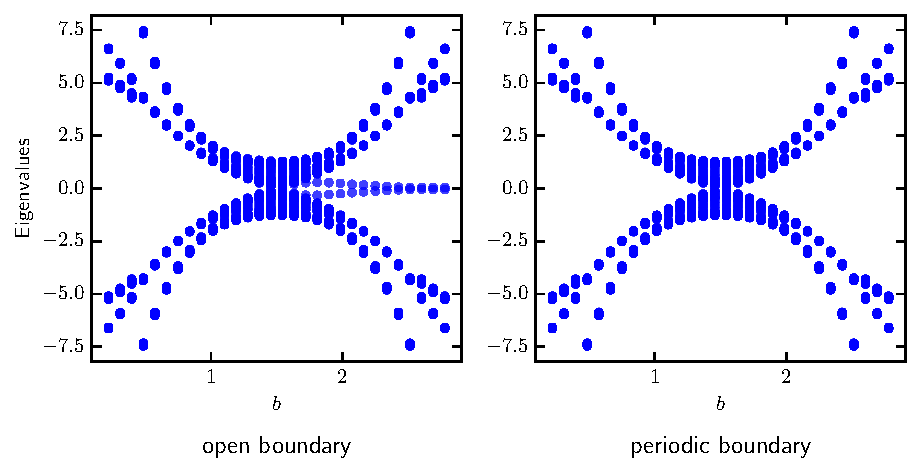
\includegraphics[scale=0.9]{pictures/aligned_dipole_in_plane_sheer_spectrum_h1.1_a3.pdf}
%     \caption{\textbf{Spectrum of almost chiral-symmetric Hamiltonian.}}
%     \label{fig:non_chiral_edge_spectrum}
% \end{figure} 



\begin{figure}[H]
    \centering
    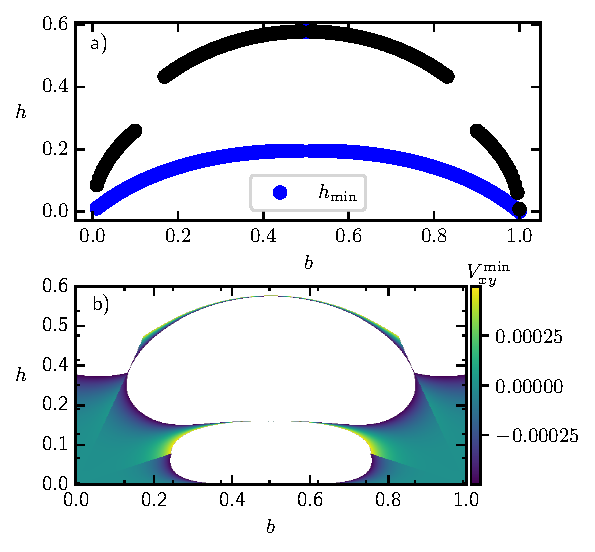
\includegraphics[]{pictures/aligned_dipoles_in_plane_sheer.pdf}
    \caption{\textbf{Optimal $h$ for chiral symmetry.} In \textbf{a)} The $h$ values are depicted which decouple $x$- and $y$-phonons. Those values were determined numerically by computing roots of $V_xy(h)$. A grid of $h$ values as initial guesses for the root algorithm was taken to have a better chance of finding all roots. In \textbf{b)} $V_xy(b,h)$ is drawn for reference. Larger values of the function have been omitted to make the pattern of small coupling values more visible.}
    \label{fig:h_for_chirality}
\end{figure} 


\begin{figure}[H]
    \centering
    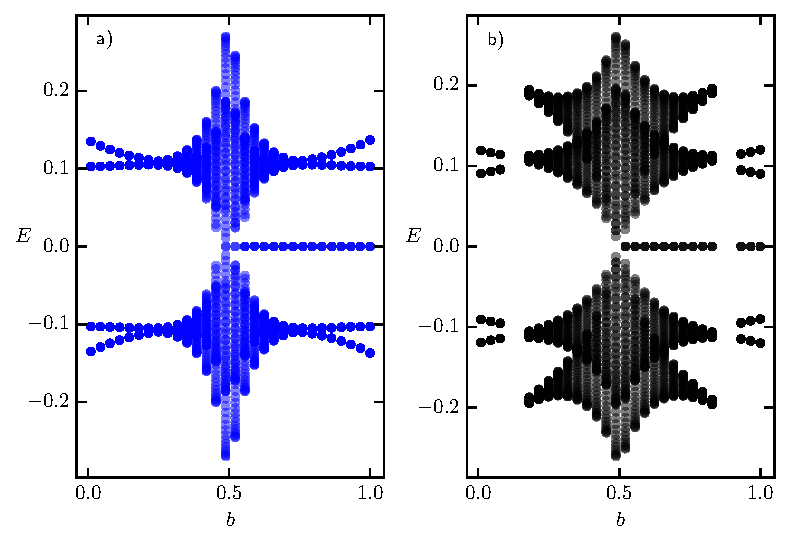
\includegraphics[]{pictures/aligned_dipoles_in_plane_sheer_spectrum_chrial.pdf}
    \caption{\textbf{Energy spectrum for the chiral Hamiltonian.}The diagram was created with the parameter $a=1$. Blue and black colors depict the Energy spectrum for the $h$ values picked from the blue and black curves in \figref{fig:h_for_chirality} respectively.}
\end{figure} 
\begin{figure}[H]
    \centering
    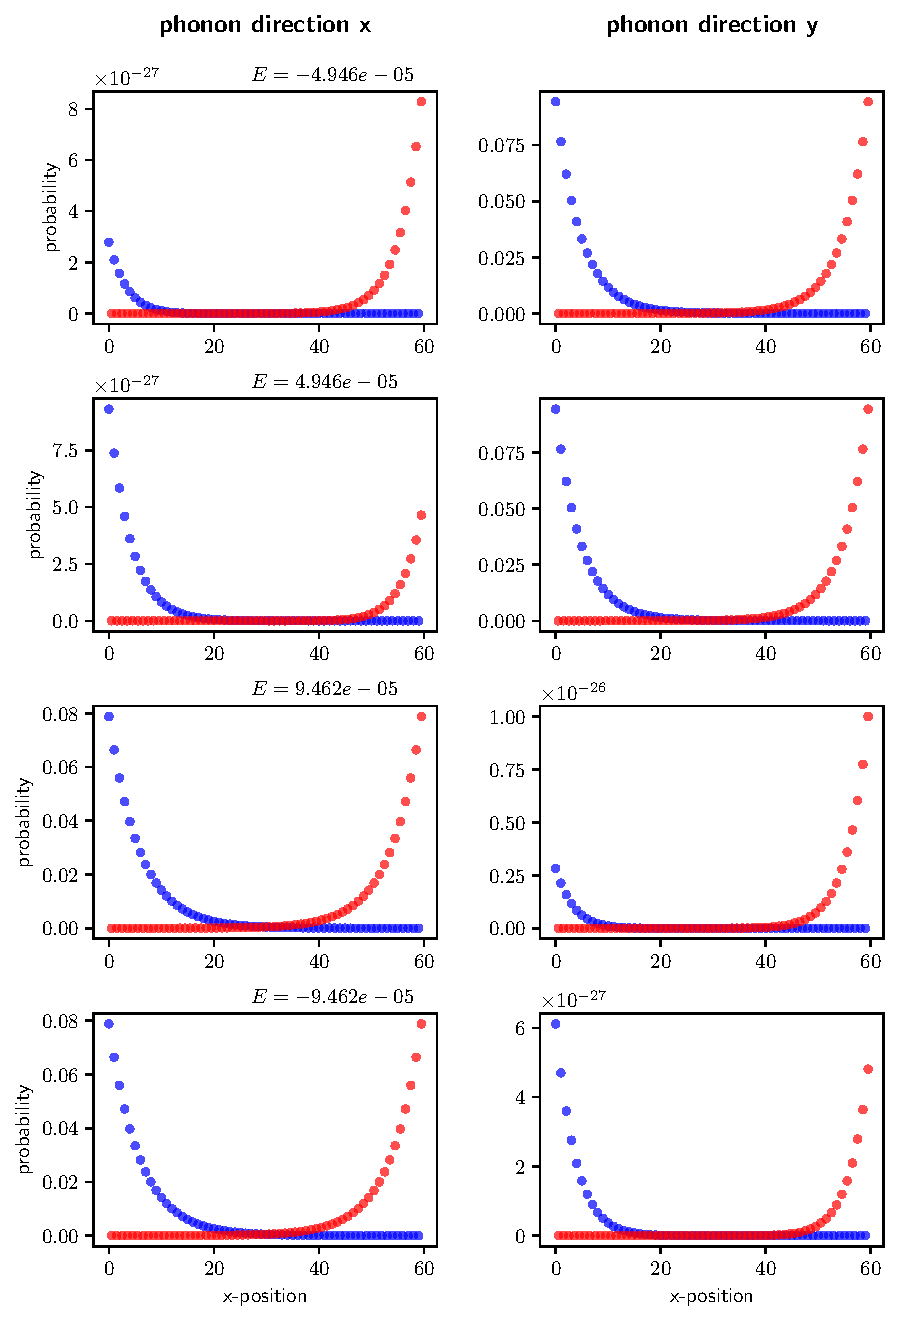
\includegraphics[]{pictures/ads_top_states_b0.51.pdf}
    \caption{\textbf{Edge states}. The figure shows the decay of edge states with the four energies with the smallest absolute value. Each row depicts one energy state. Drawn in blue are the excitations of sublattice A, while the excitation of sublattice B is shown in red.}
\end{figure} 
\begin{figure}[H]
    \centering
    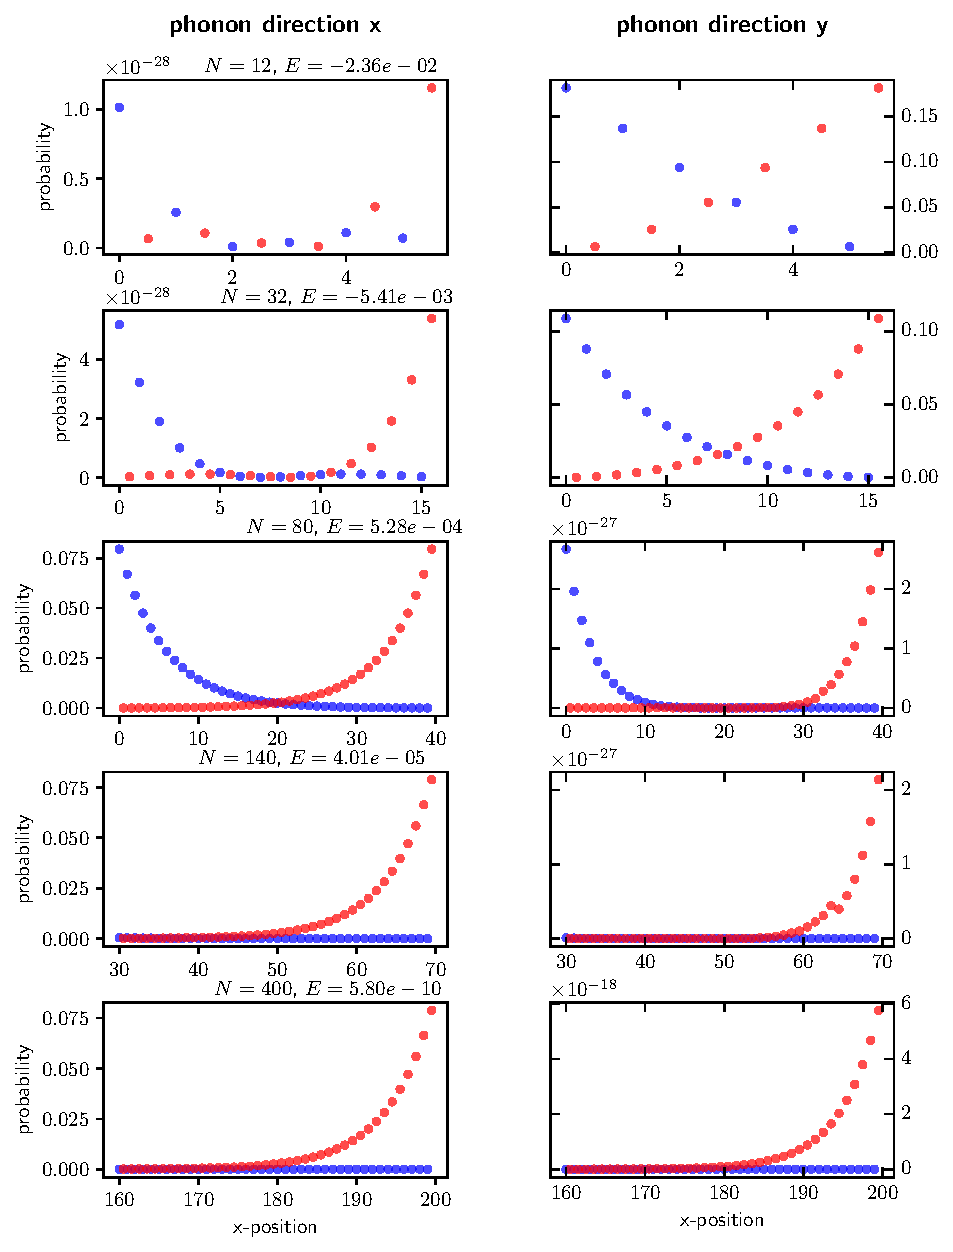
\includegraphics[]{pictures/ads_states_for_chain_lengths.pdf}
    \caption{\textbf{Decay of energy for topological states with atom number.}. In each row the eigenstate for the energy with smallest absolute value is plotted. Blue and red show again the excitations of sublattice A and B respectively. When moving down in the rows of the figure the atom number of the system is increased. It shows that with increasing atom number the energy of the topological decays. What also can be observed. That the decay-length of the excitations when moving away from the edges does not change with particle number.}
\end{figure} 
\begin{figure}
    \centering
    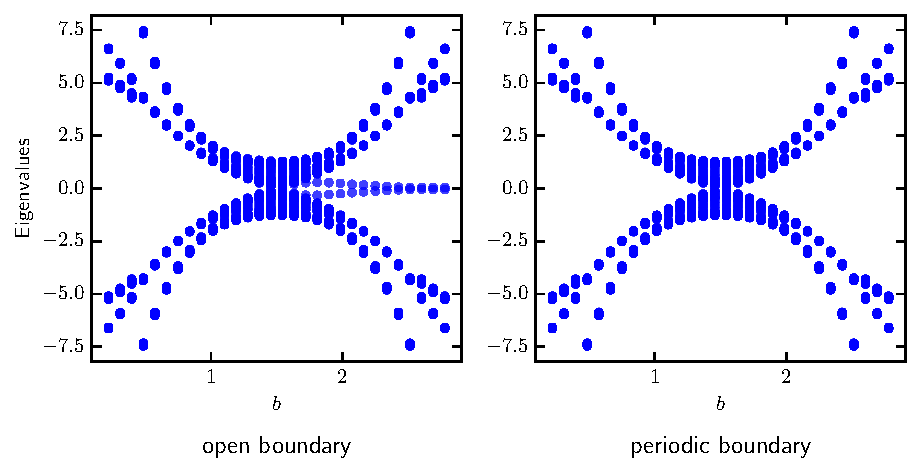
\includegraphics[scale=0.9]{pictures/aligned_dipole_in_plane_sheer_spectrum_h1.1_a3.pdf}
\end{figure} 
\begin{figure}
    \centering
    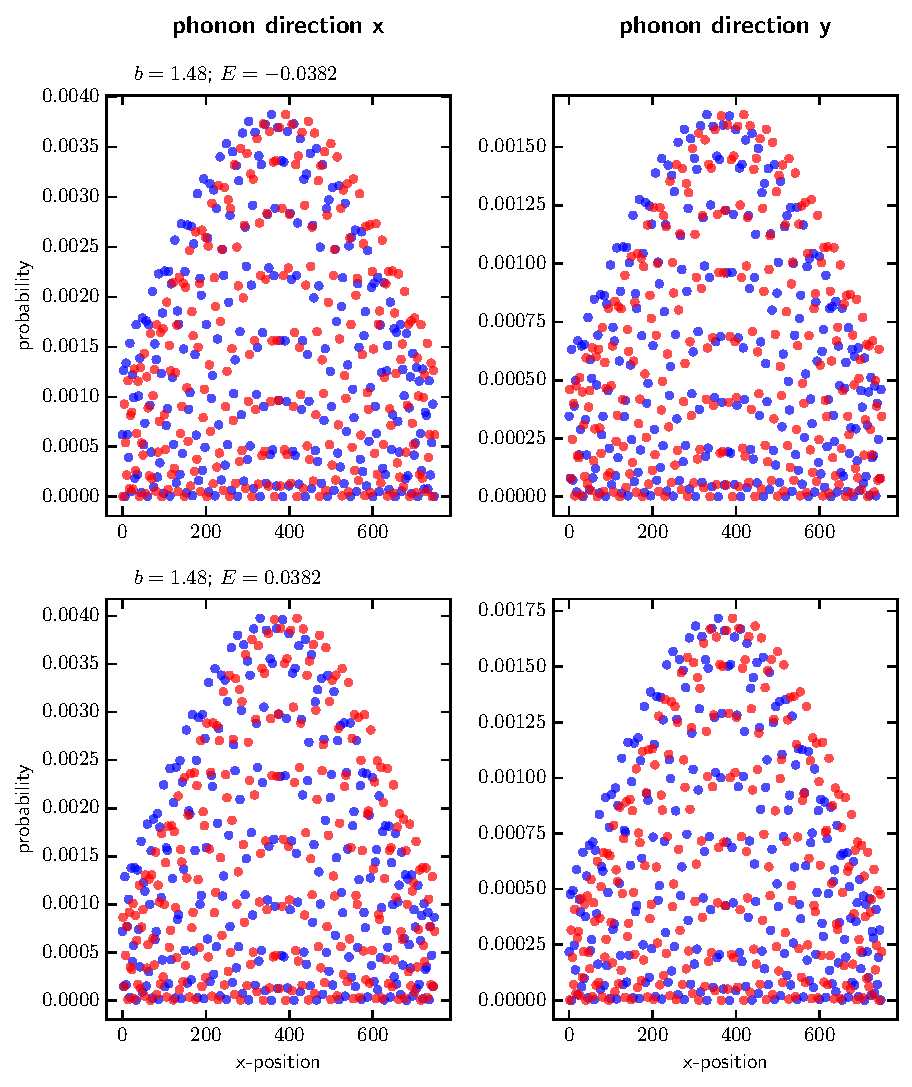
\includegraphics[scale=0.85]{pictures/aligned_dipoles_in_plane_sheer_h1.1_a3_eigenvecs0.pdf}
\end{figure} 
\begin{figure}
    \centering
    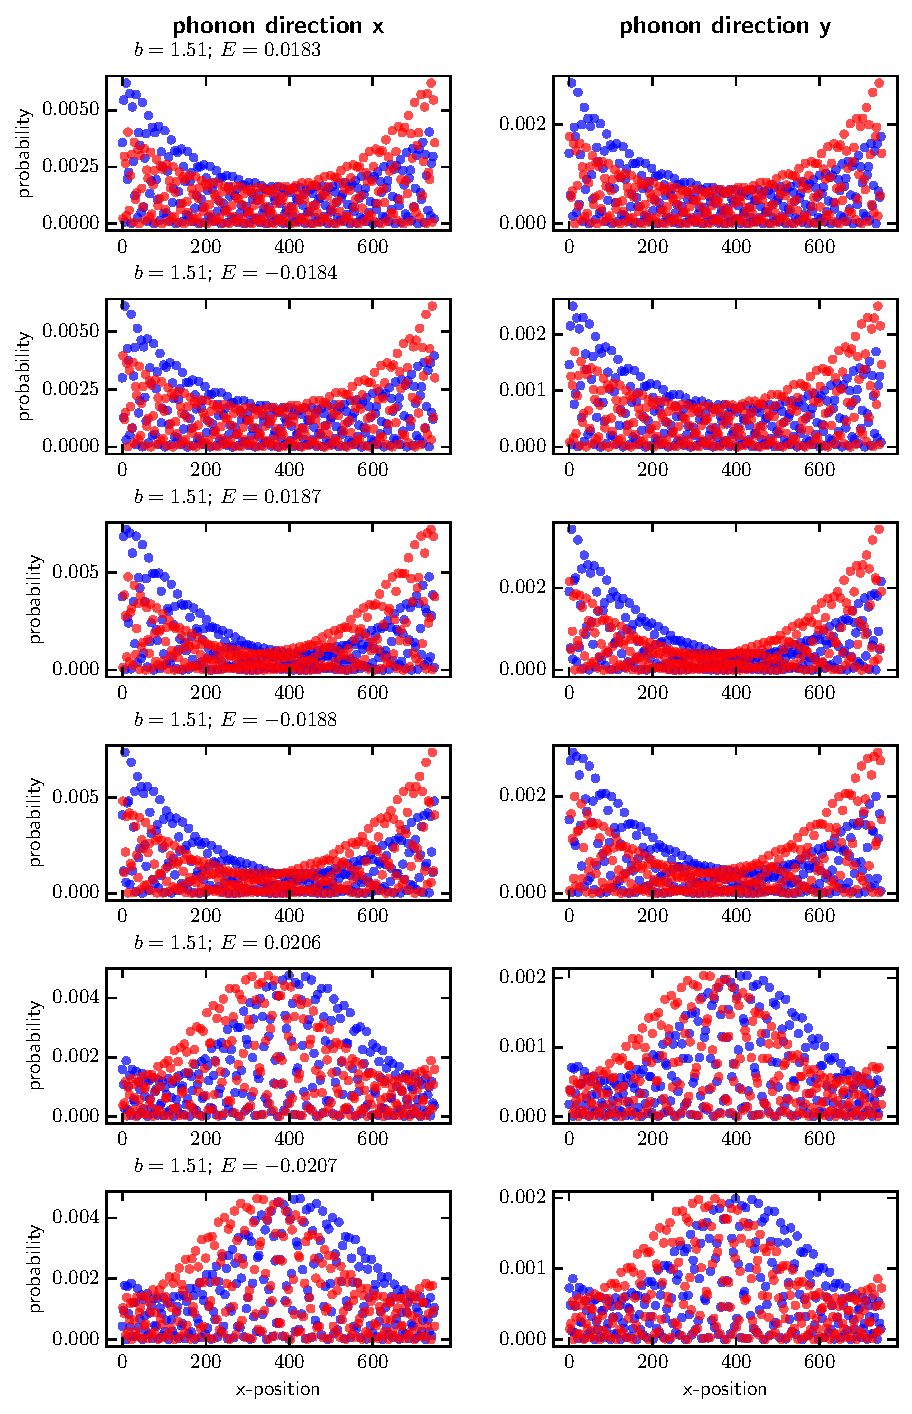
\includegraphics[]{pictures/aligned_dipoles_in_plane_sheer_h1.1_a3_eigenvecs1.pdf}
\end{figure}
\begin{figure}
    \centering
    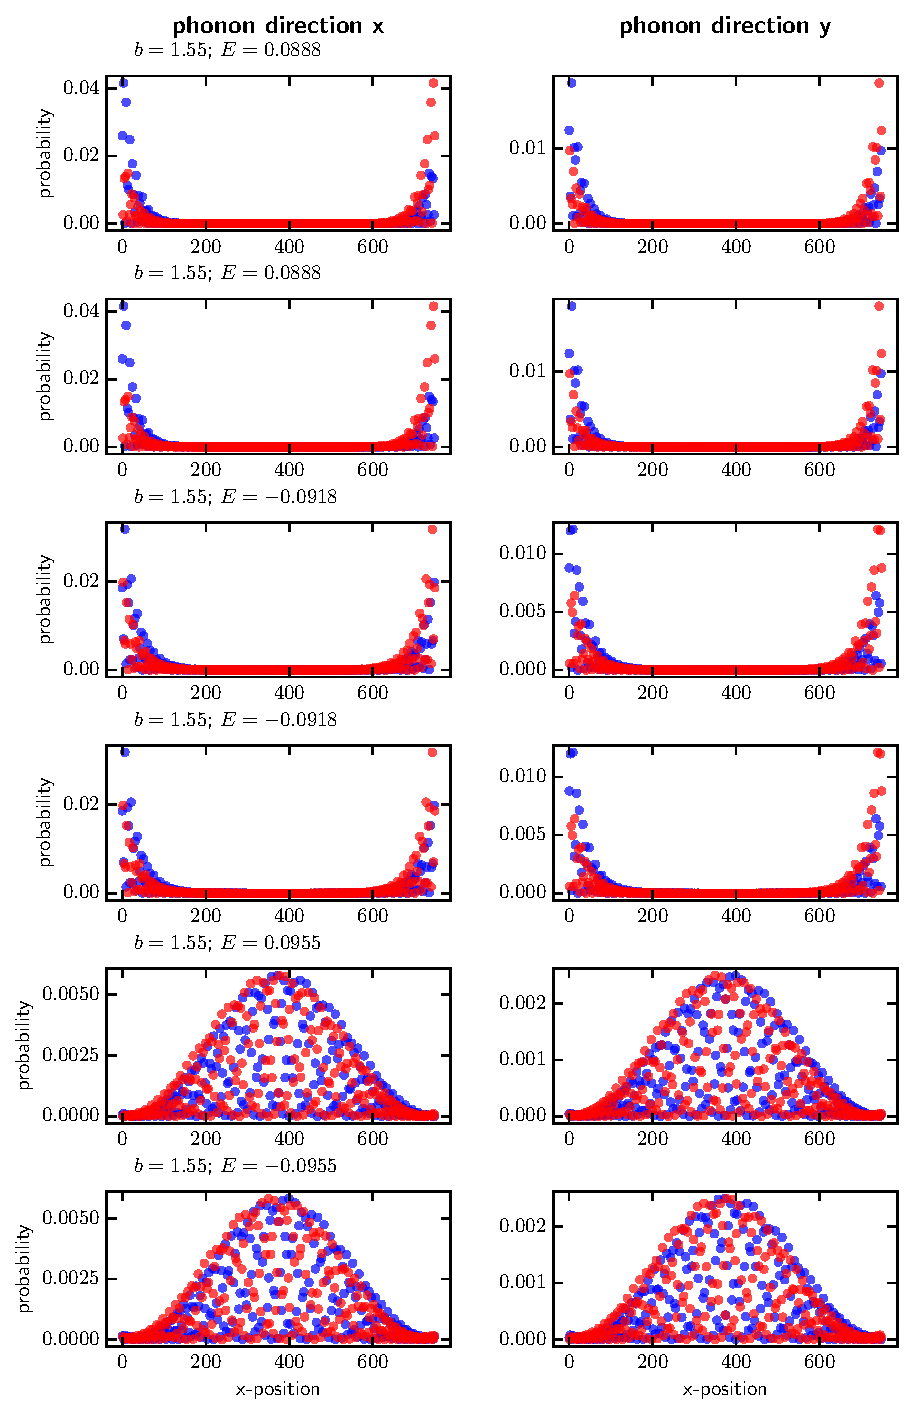
\includegraphics[]{pictures/aligned_dipoles_in_plane_sheer_h1.1_a3_eigenvecs2.pdf}
\end{figure}

\begin{figure}
    \centering
    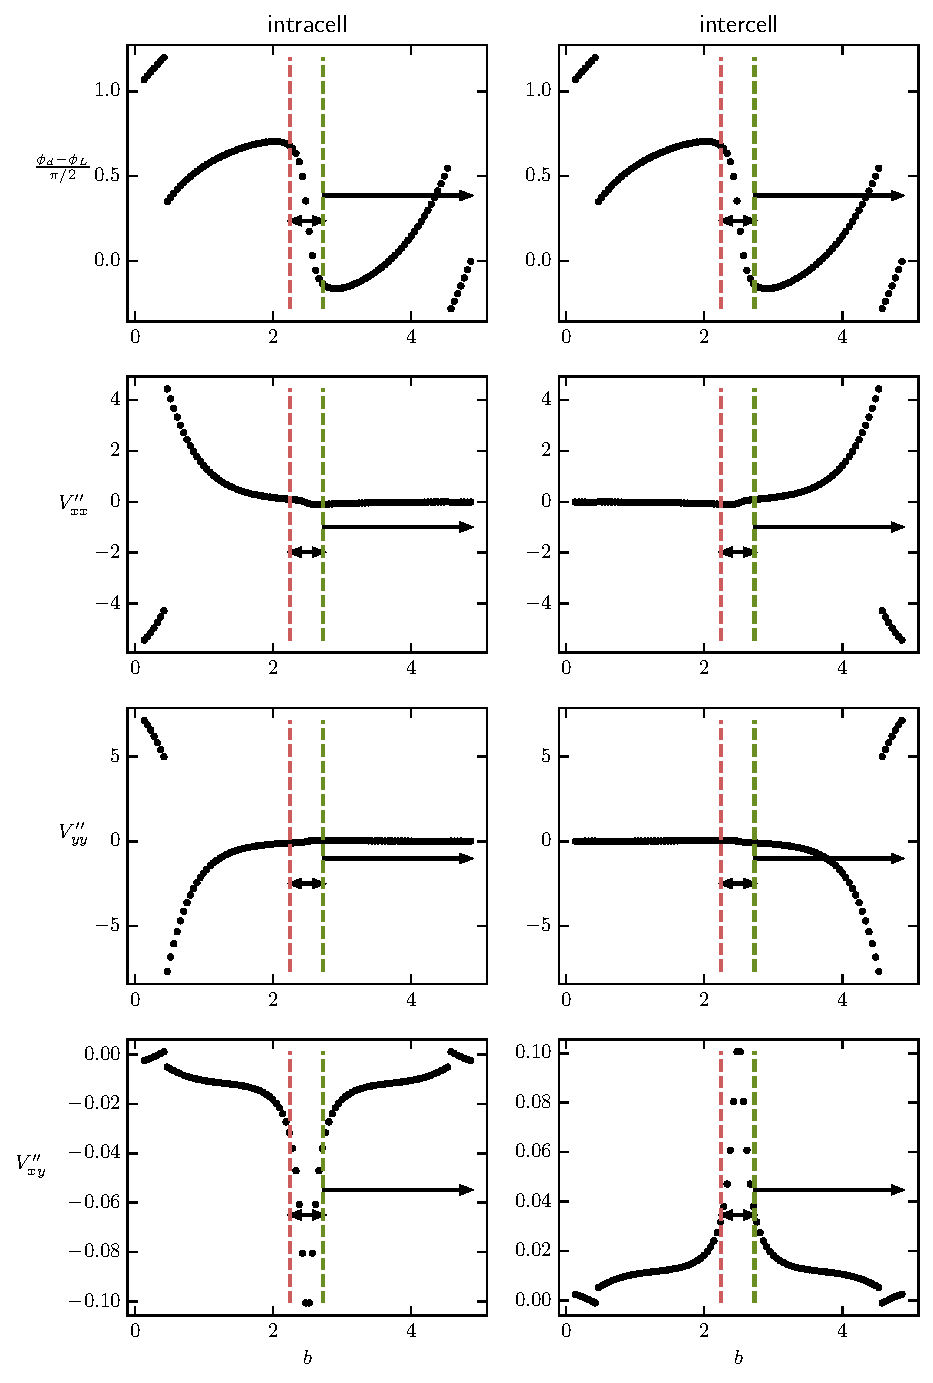
\includegraphics[]{pictures/aligned_dipoles_in_plane_orientation_sheer_h1.1_a5.pdf}
    \caption{The diagram was created with the parameters $a=5$, $h=1.1$. Between the red and the olive dashed line, i.e. bewteen $b$-values of $2.25$-$2.73$ the winding number is 1, whereas right to the olive dashed line the winding number is 2.}
\end{figure} 
\begin{figure}
    \centering
    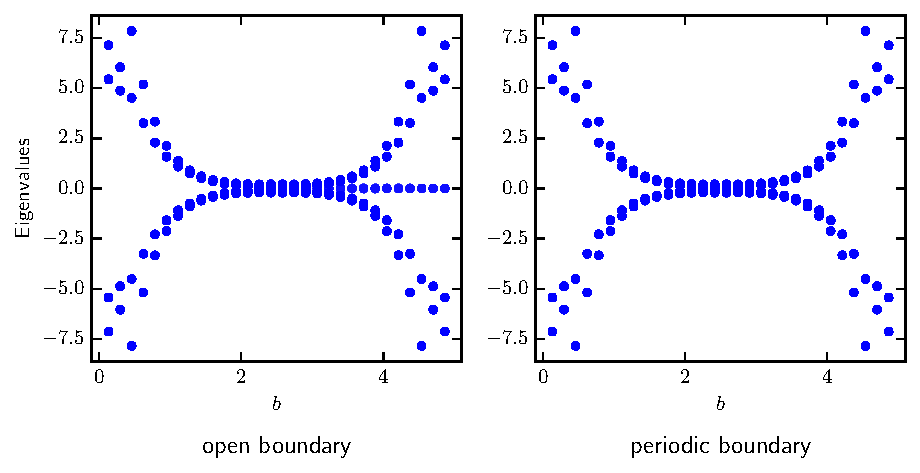
\includegraphics[scale=0.9]{pictures/aligned_dipole_in_plane_sheer_spectrum_h1.1_a5.pdf}
\end{figure} 
\begin{figure}
    \centering
    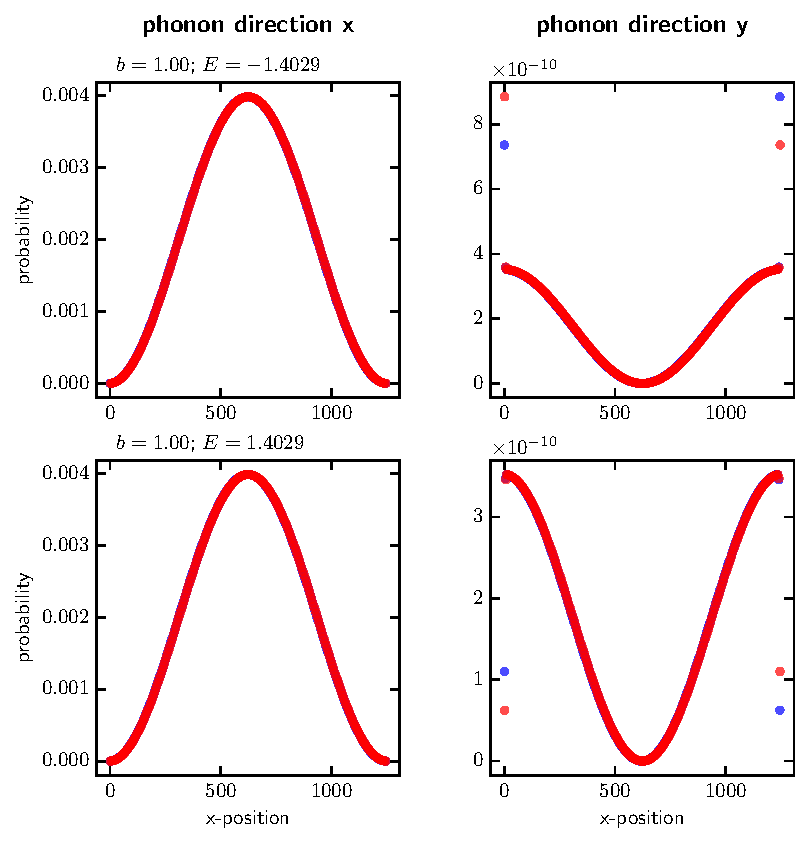
\includegraphics[]{pictures/aligned_dipoles_in_plane_sheer_h1.1_a5_eigenvecs0.pdf}
\end{figure} 
\begin{figure}
    \centering
    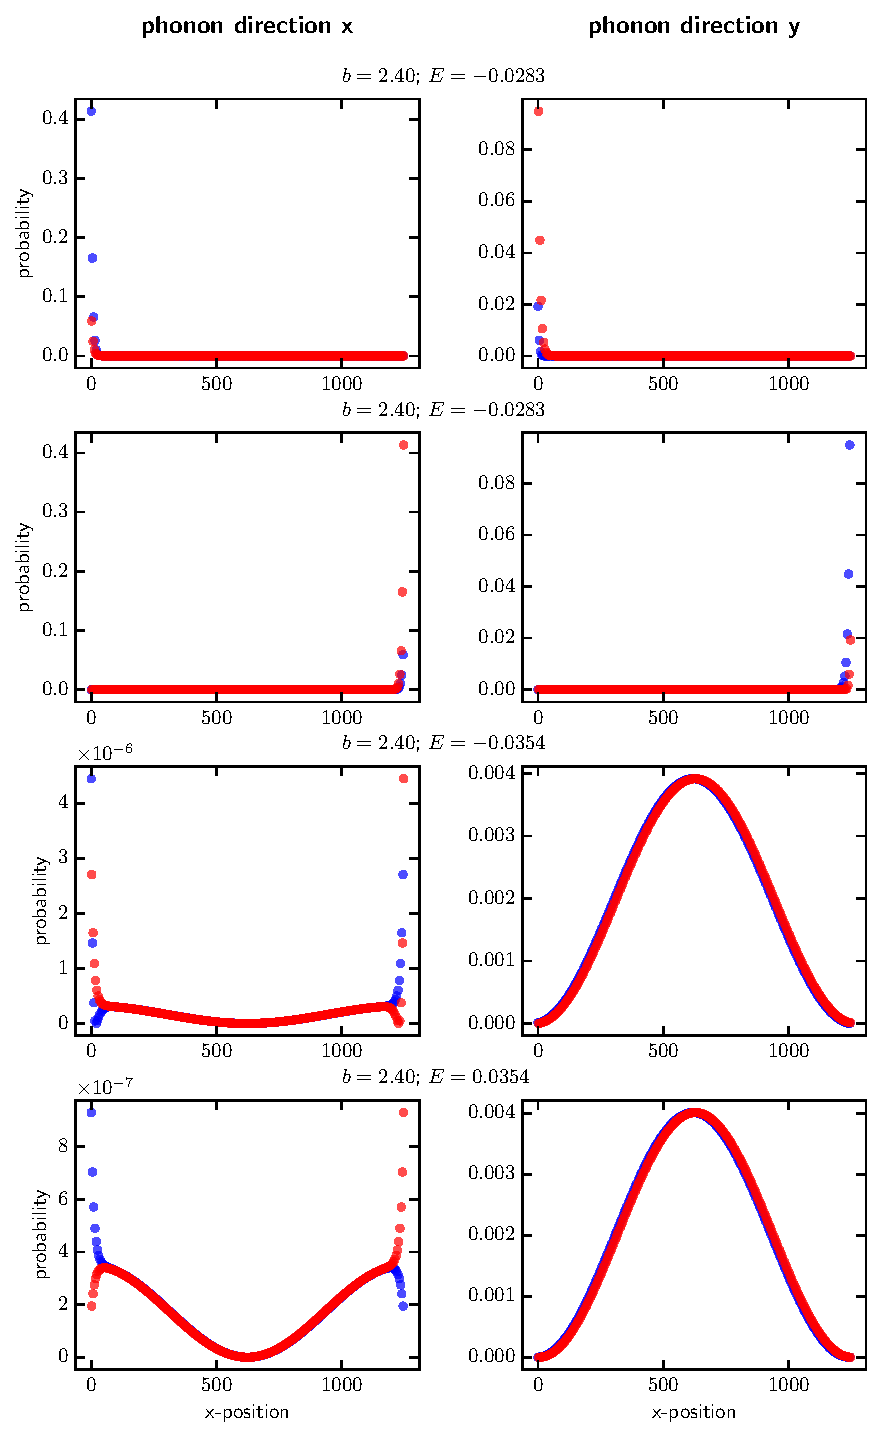
\includegraphics[]{pictures/aligned_dipoles_in_plane_sheer_h1.1_a5_eigenvecs1.pdf}
\end{figure}
\begin{figure}
    \centering
    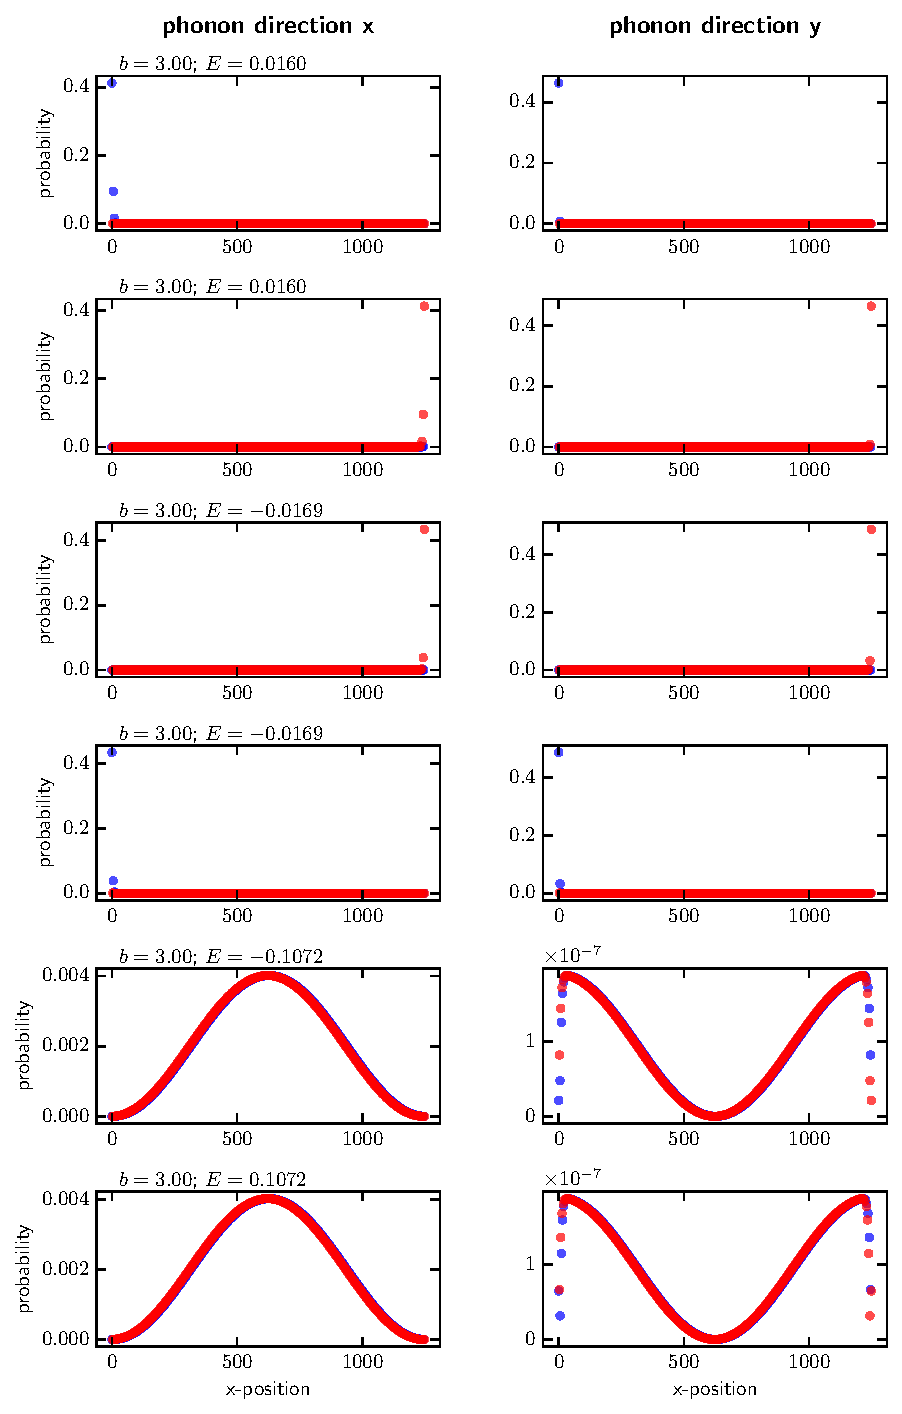
\includegraphics[]{pictures/aligned_dipoles_in_plane_sheer_h1.1_a5_eigenvecs2.pdf}
\end{figure}

\subsection*{Out of plane dipoles}
First I will allow the dipoles to point out of the $xy$-plane in which the one dimensional chain will reside. I restrict the dipoles to the following form in order to have easier calcualtions.
\begin{align*}
    \mathbf{d}_1= \begin{pmatrix}
        d_{1,x}\\
        0\\
        \sqrt{-d_{1,x}^2}
    \end{pmatrix},\quad
    \mathbf{d}_2= \begin{pmatrix}
        0\\
        d_{2,y}\\
        \sqrt{-d_{2,y}^2}
    \end{pmatrix}
\end{align*}
\begin{figure}[H]
    \centering
    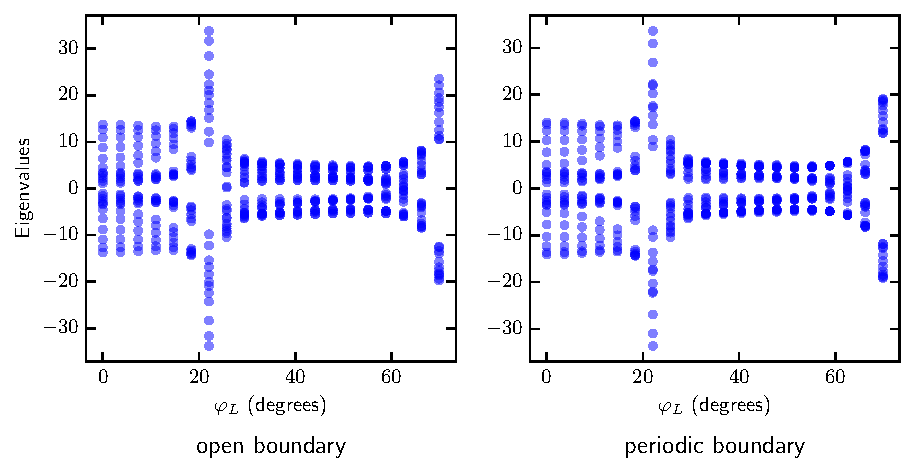
\includegraphics[]{pictures/out_of_plane_dipole_orientation_zigzag.pdf}
\end{figure}
\begin{figure}[H]
    \centering
    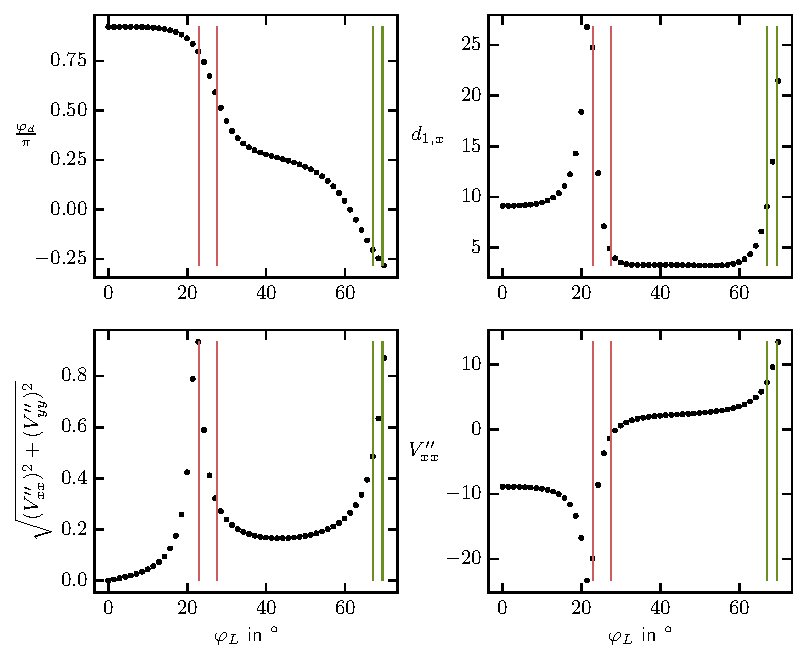
\includegraphics[]{pictures/dipole_orientation_off_plane.pdf}
    \caption{The occurance of topological states is signaled by the vertical lines. Between the two red as well as between the two green lines topological states can be found.}
\end{figure}%
As chain I consider a zig-zag chain with sublattice vector $\mathbf{a}_S$ and lattice vector $\mathbf{a}_L$.
\begin{align*}
    \mathbf{a}_S = \begin{pmatrix}
        c\\
        \epsilon
    \end{pmatrix},\quad\mathbf{a}_L = \begin{pmatrix}
        c+1\\
        0
    \end{pmatrix}
\end{align*}
For nearest neighbour interaction the condition that lets the momentum space Hamiltonian be chiral under periodic boudary conditions reads
\begin{align*}
    0&\overset{!}{=}V''_{xy}(\mathbf{a}_S)+V''_{xy}(\mathbf{a}_S-\mathbf{a}_L)\\
    V''_{xy}(\mathbf{r}_0)&\vcentcolon=\frac{\partial^2 V}{\partial r_x\partial r_y}(\mathbf{r}_0)
\end{align*}

With the particular dipole configuration, introduced above, the derived interaction takes the form
\begin{align*}
    V''_{xy}(\mathbf{r})&=d_{1,x}d_{2,y}\,\left( \frac{12}{r^5}-105\,\frac{r_x^2r_y^2}{r^9} \right)+15\,\sqrt{1-d_{1,x}^2}\,\sqrt{1-d_{2,y}^2}\,\frac{r_xr_y}{r^7}\\
    V''_{\alpha\alpha}(\mathbf{r})&=d_{1,x}d_{2,y}\,\left( 45\,\frac{r_xr_y}{r^7} - 105\,r_\alpha^2\,\frac{r_xr_y}{r^9} \right)+\sqrt{1-d_{1,x}^2}\,\sqrt{1-d_{2,y}^2}\,\left( -\frac{3}{r^5}+15\,\frac{r_\alpha^2}{r^7} \right)
\end{align*}


\subsection*{In plane dipole orientation}
As a next step I restrict the dipoles to the $xy$-plane seperate the magnitude of the dipole projected onto the plane from the occurance of topological states. In this scenario I investigate the properties of the dipole restriction of the following form.
\begin{align*}
    \mathbf{d}_1= \begin{pmatrix}
        d_{1,x}\\
        d_{1,y}\\
        0
    \end{pmatrix},\quad
    \mathbf{d}_2= \begin{pmatrix}
        d_2\\
        0\\
        0
    \end{pmatrix}
\end{align*}
For this configuration the interaction takes to From
\begin{align*}
    V''_{xy}(\mathbf{r})&=d_{1,x}d_2\,\left( 45\,\frac{r_xr_y}{r^7}-105\,\frac{r_x^3r_y}{r^9} \right)+ d_{1,y}d_2\,\left( \frac{12}{r^5}-105\,\frac{r_x^2r_y^2}{r^9} \right)\\
    V''_{\alpha\alpha}(\mathbf{r})&=d_{1,x}d_2\,\left[ -\frac{3+\delta_{\alpha,x}}{r^5}+\frac{15}{r^7}\,\left( r_x^2 + 2\,r_\alpha r_x+r_\alpha^2+2\delta_{\alpha,x}\,r_x^2\right) -105\,\frac{r_x^2\,r_\alpha^2}{r^9} \right]\\
    &+ d_{1,y}d_2\,\left[ \frac{15}{r^7}\,\left( r_xr_y + 2\delta_{\alpha,x}\,r_xr_y\right)-105\,\frac{r_\alpha^2r_xr_y}{r^9} \right]
\end{align*}

\begin{figure}[H]
    \centering
    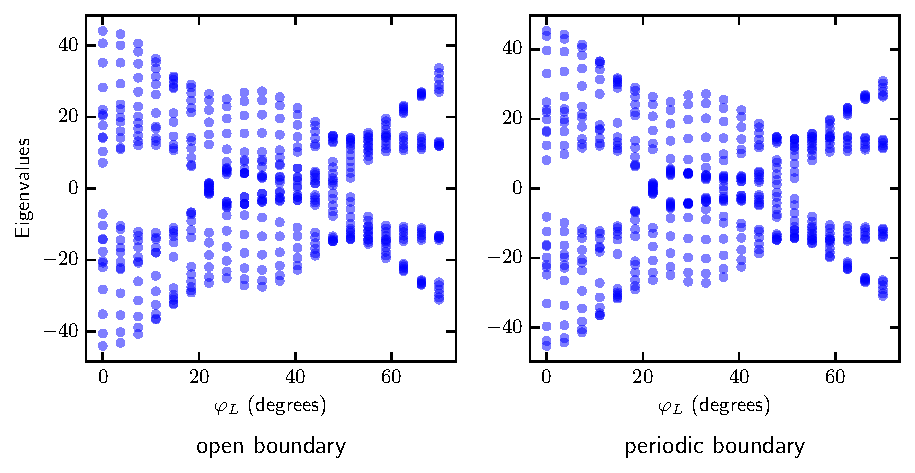
\includegraphics[]{pictures/inplane_dipole_orientation_zigzag.pdf}
\end{figure} 
\begin{figure}[H]
    \centering
    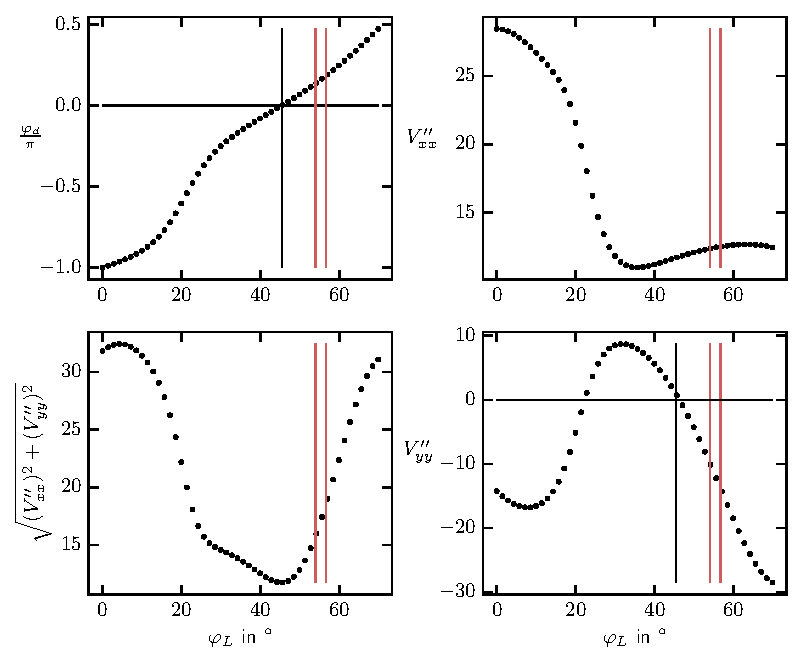
\includegraphics[]{pictures/dipole_orientation_in_plain.pdf}
    \caption{Topological states can again be found in the angle range between the two red vertical lines.}
\end{figure}

\subsection*{1D hexagonal chain}
In this chapter I consider a chain with equal spacing $r$ between the atoms where the angle $\varphi$ is changed in a manner, such that the first layer of a 2D hexagonal lattice is reached. Because of the one dimensionality of the chain the unit cell contains four atoms (A, B, C, D).
\begin{align*}
    \mathbf{a}_L&=\begin{pmatrix}
        2r\,(1+\cos\varphi_L)\\0
    \end{pmatrix}\quad\mathbf{a}_B=\begin{pmatrix}
        r\cos\varphi_L\\r\sin\varphi_L
    \end{pmatrix}\\
    \mathbf{a}_C&=\begin{pmatrix}
        r\,(1+\cos\varphi_L)\\r\sin\varphi_L
    \end{pmatrix}\quad\mathbf{a}_D=\begin{pmatrix}
        r\,(1+2\cos\varphi_L)\\0
    \end{pmatrix}
\end{align*}

\begin{figure}[H]
    \centering
    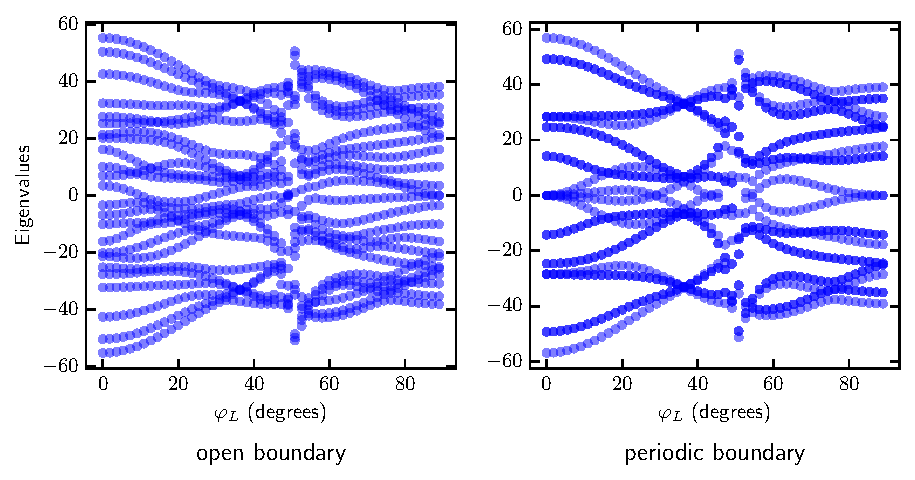
\includegraphics[]{pictures/in_plane_dipole_orientation_hex1D.pdf}
\end{figure} 
\begin{figure}[H]
    \centering
    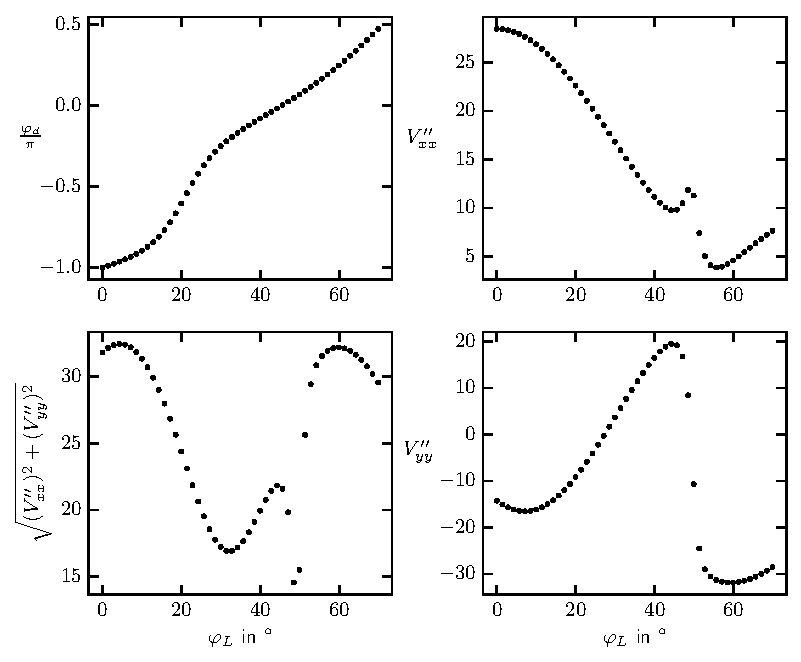
\includegraphics[]{pictures/dipole_orientation_in_plane_hex1D.pdf}
    \caption{In this configuration with equal spacing between the atoms no topological states occur.}
\end{figure}

\section{Aligned dipoles in plane}
\begin{figure}[H]
    \centering
    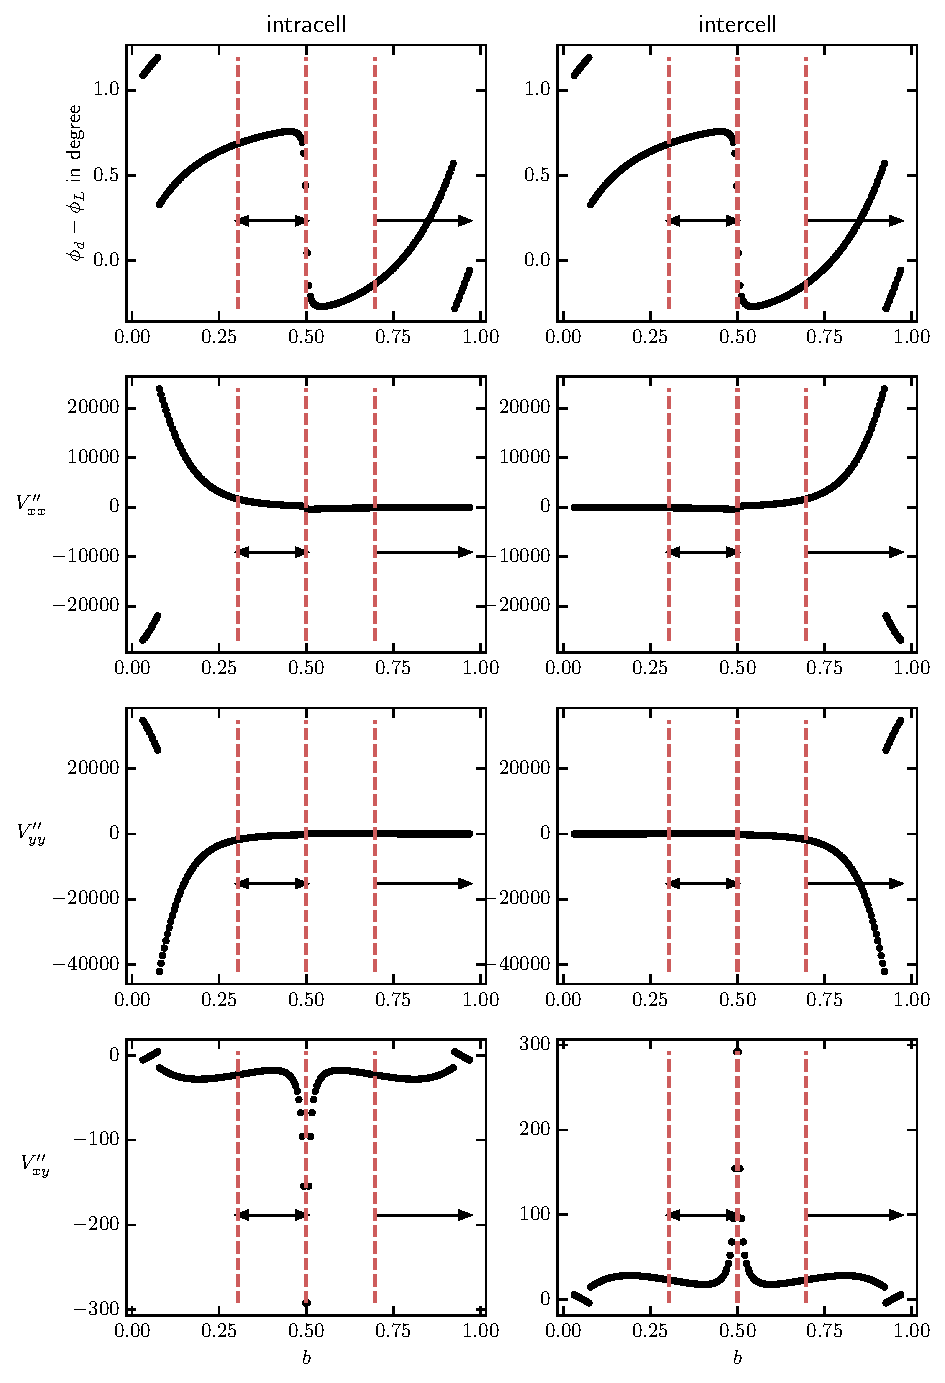
\includegraphics[]{pictures/aligned_dipoles_in_plane_zigzag_h0.2.pdf}
\end{figure} 
\begin{figure}[H]
    \centering
    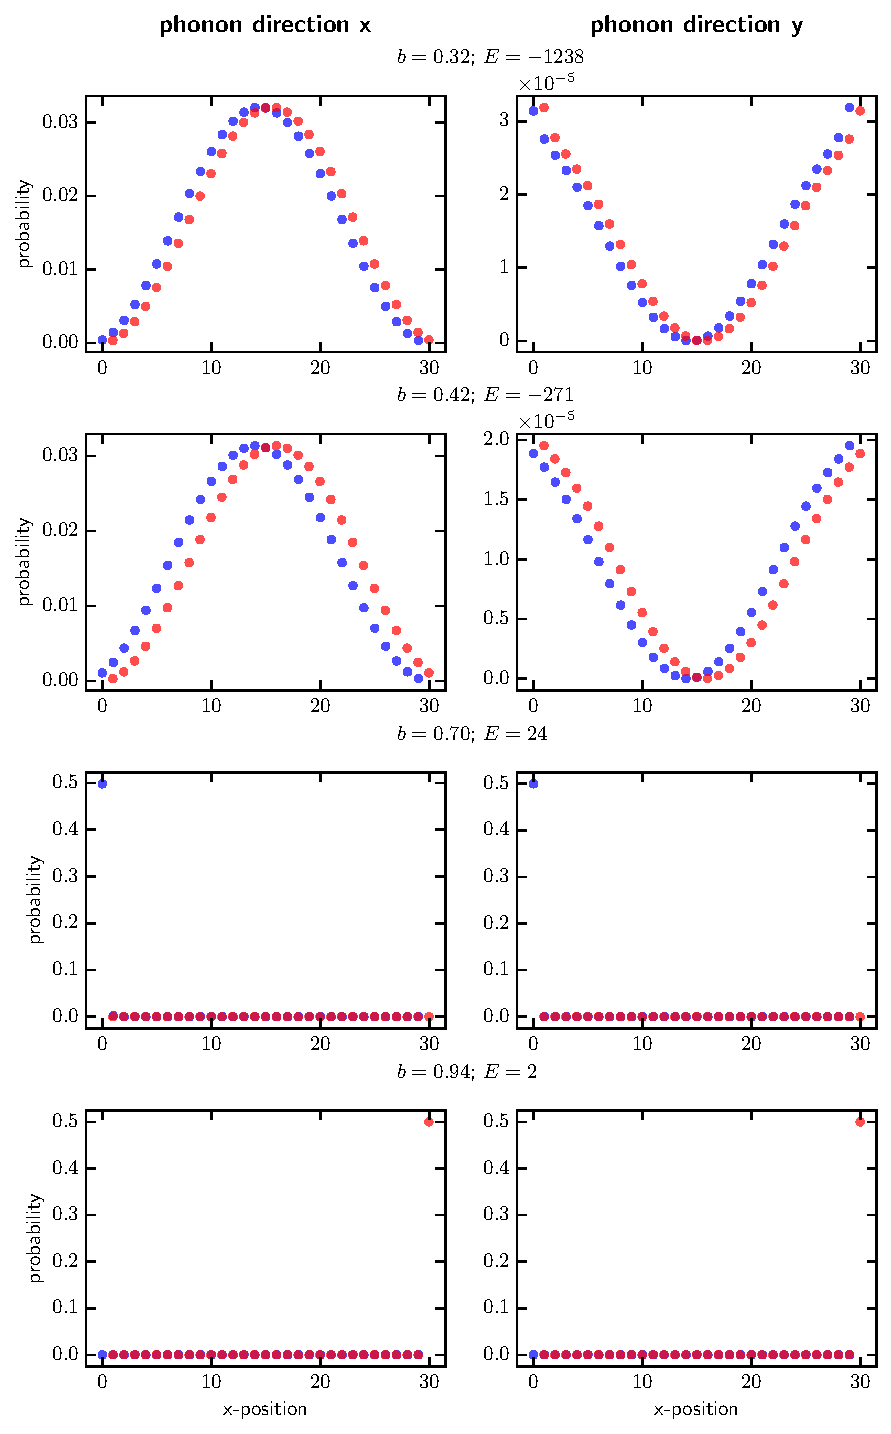
\includegraphics[]{pictures/aligned_dipoles_in_plane_zigzag_h0.2_eigenvecs.pdf}
\end{figure} 
\begin{figure}[H]
    \centering
    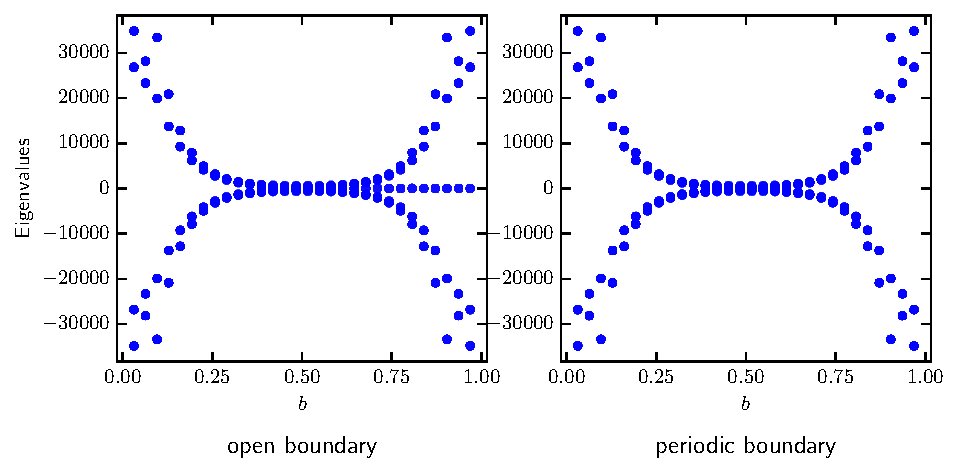
\includegraphics[]{pictures/aligned_dipole_in_plane_zigzag_spectrum_h0.2.pdf}
\end{figure} 
\begin{figure}[H]
    \centering
    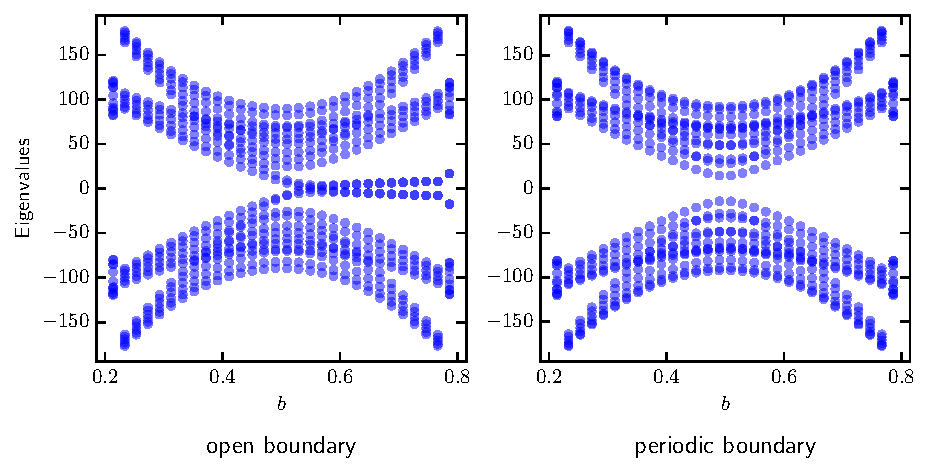
\includegraphics[]{pictures/aligned_dipole_in_plane_zigzag_spectrum_h0.6.pdf}
\end{figure} 
\begin{figure}[H]
    \centering
    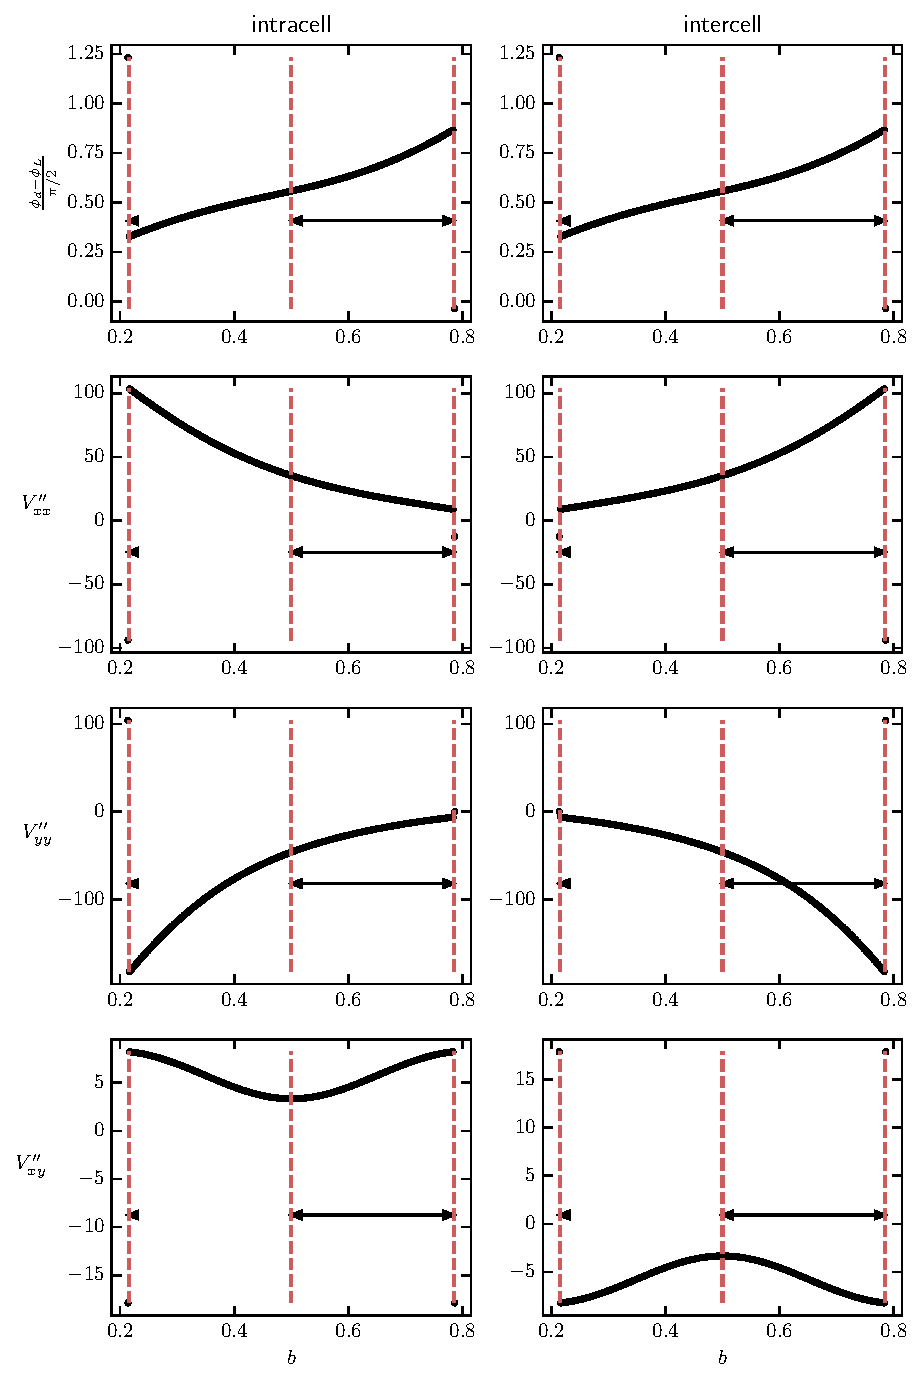
\includegraphics[]{pictures/aligned_dipoles_in_plane_zigzag_h0.6.pdf}
\end{figure} 
\begin{figure}[H]
    \centering
    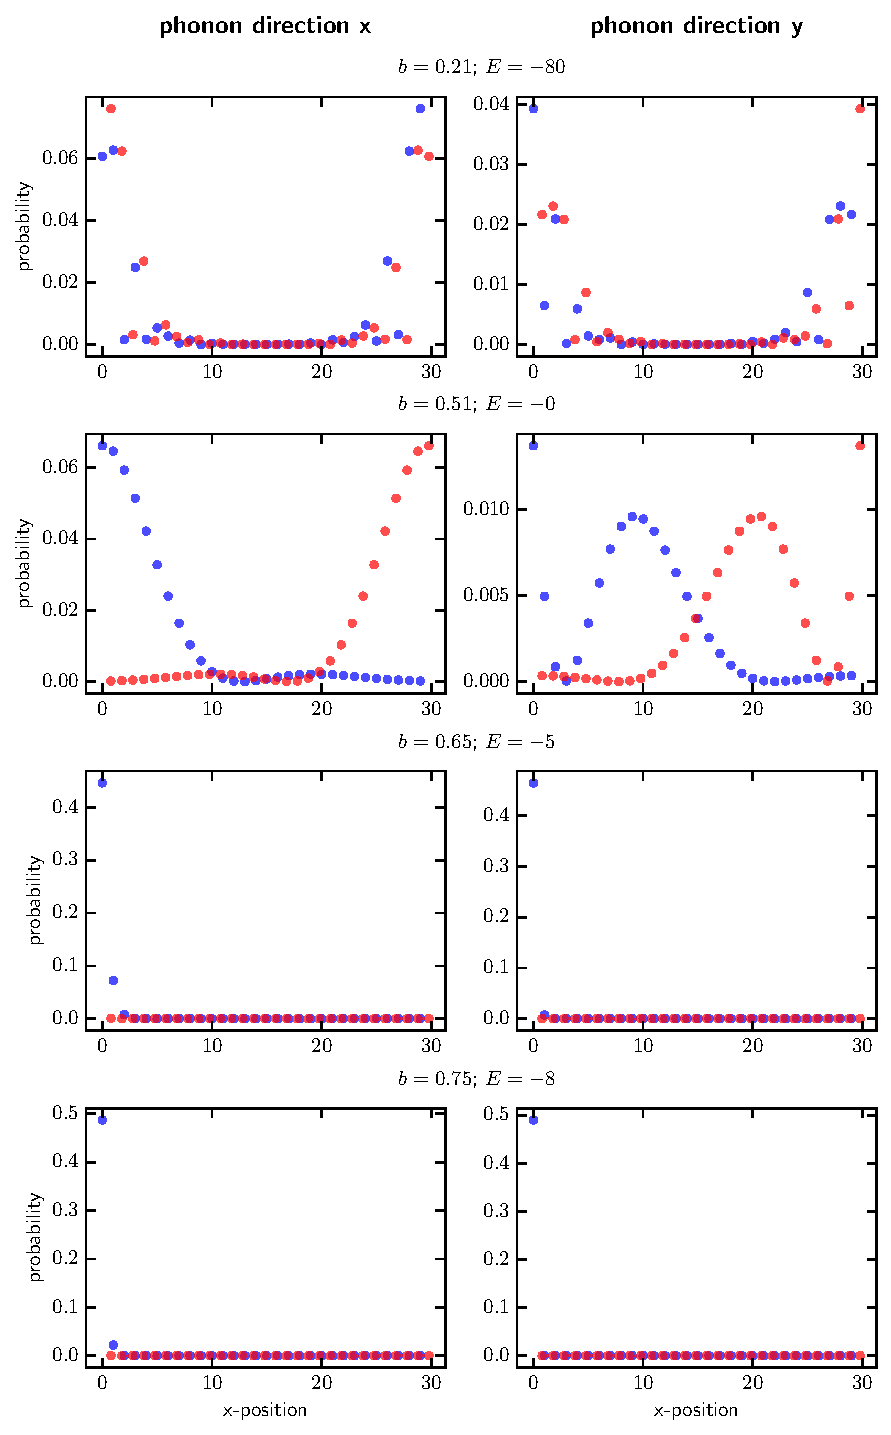
\includegraphics[]{pictures/aligned_dipoles_in_plane_zigzag_h0.6_eigenvecs.pdf}
\end{figure} 


\section{1D chain}
When allowing displacements in the 2-dimensional plane one can exploit the independence of the individual contributions to $H_k$, which implies that $X$ has to anti-commute with every contribution individually. Due to the results of \appref{appendix:symmetry} the only possible chiral symmetry in the case where $H_k^{A,A}$ is not identical zero is represented by the unitary
\begin{align*}
    S= \mathbb{1}\otimes\sigma_y
\end{align*}
It requires that the identity contribution in the second slot of the tensor product has to vanish. This can only be true if the $xx$ and $yy$ interaction have opposite signs.
% The first consequence is, that $H_k$ can not contain a term proportional to the identity. Thus $(H_k^{A,A})_0=0$ referring to the notation of \eqref{eq:xy-decomposition}. %The identity 
% % \begin{align*}
% %     \{\sigma_i\otimes\sigma_j,\sigma_n\otimes\sigma_m\}=\half\,\{\sigma_i,\sigma_n\}\otimes\{\sigma_j,\sigma_m\}
% % \end{align*}
% % which is derived in \secref{appendix:symmetry}, infers that possible contributions to an anti-commuting matrix $X$ contain
% % \begin{align*}
% %     \sigma
% % \end{align*}
% This term is determined by the interactions between sites of the same sublattice and modes of the same direction of displacement, i.e. $xx$ or $yy$, and the onsite term of $U$. The fact that $(H_k^{A,A})_0=0$ has to hold for all $k$ enforces the onsite term $U_{ii}^{\alpha,\alpha}=\sum_r\partial^2V_{dd}/\partial r_\alpha^2$ to be zero or have opposite sign for the two displacement directions. 
% Exploiting the high control of dipole traps in cold atom experiments one can tune the harmonic potential of each trap individually \cite{endresAtombyatomAssemblyDefectfree2016,youngHalfminutescaleAtomicCoherence2020}.
% Thus by fine tuning the trap frequencies at each site one can in principle cancel the onsite terms.

% At the same time one has to take into consideration that these conditions also have to be true at the borders of the chain, as in order for the bulk-boundary correspondence to be applicable both the infinite system as well as the open system have to respect the necessary symmetries. Thus if one wants to implement a system where the sum in the onsite potential vanishes, one has to make sure that the two parts of the sum, going to the right and to the left, vanish individually. Because of the vast decay of the interaction with $1/r^5$ I only considered up to next nearest neighbor interactions. In this case it was not possible to find a dipole orientation that meets the condition of vanishing onsite potential.
% Consequently I resort to the second possibility, to make interactions between $xx$ and $yy$ of opposite sign. 
Recall the dependence of the interaction of the direction of $\mathbf{r}$ and $\mathbf{d}$ in form of   
% Thus either the interactions inside a sublattice between the same direction have to vanish or the $xx$ and $yy$ interactions have to have opposite sign, allowing the $(H_k^{A,A})_0$ term to be non-zero. In the first case one has to tune the interactions between sites of the same sublattice to zero. But the onsite term $U_{ii}^{\alpha,\alpha}=\sum_r\partial^2V_{dd}/(\partial r_\alpha \partial r_\alpha)$ has to be considered as well. As the 

\begin{align*}
    c_{\alpha\beta}(\hat{\mathbf{r}}) &= \delta_{\alpha\beta}\left(-3 + 15\, (\hat{\mathbf{r}}\cdot \hat{\mathbf{d}})^2\right)- 6\,\hat{d}_\alpha \hat{d}_\beta +30\, \frac{\hat{d}_\alpha r_\beta + \hat{d}_\beta r_\alpha}{r}\,(\hat{\mathbf{r}}\cdot \hat{\mathbf{d}}) + 15\,\frac{r_\alpha r_\beta}{r^2} \left(1  - 7\, (\hat{\mathbf{r}}\cdot \hat{\mathbf{d}})^2\right)\\
    &= \delta_{\alpha\beta}\left(-3 + 15\, (\hat{\mathbf{r}}\cdot \hat{\mathbf{d}})^2\right) + A_{\alpha\beta}
\end{align*}
\begin{figure}[h]
    \hspace*{-2cm}
    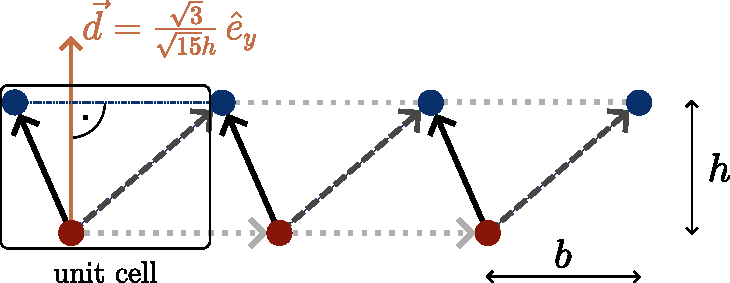
\includegraphics{pictures/chain_with_interaction_arrows2.pdf}
    \caption{\textbf{Zik-zak chain and dipole orientation.} Interactions up to next nearest neighbors are presented. The dipole is orientated in such a way that it is perpendicular to the connection vectors of nearest neighbor distances. Thus the scalar product with the dipole moment is the same for both the solid and the dashed vector.}
    \label{fig:chain and dipole orientation}
\end{figure}
% \hfill\newpage
In order for the interaction between atoms of relative distance $\mathbf{r}$ to vanish the following condition has to hold
\begin{align}\label{eq:opposite sign condition}
    c_{xx}(\hat{\mathbf{r}})&\overset{!}{=}-c_{yy}(\hat{\mathbf{r}})\\
    &=-6 + 30 \, (\hat{\mathbf{r}}\cdot \hat{\mathbf{d}})^2 + A_{xx}+A_{yy}\notag\\
    A_{xx}+A_{yy}&=- 6\,(\hat{d}_x^2+\hat{d}_y^2) +60\, \frac{\hat{d}_x r_x + \hat{d}_y r_y}{r}\,(\hat{\mathbf{r}}\cdot \hat{\mathbf{d}}) + 15\,\frac{r_x^2 + r_y^2}{r^2} \left(1  - 7\, (\hat{\mathbf{r}}\cdot \hat{\mathbf{d}})^2\right)\notag\\
    &= 9\,||d_{\parallel}||^2 - 3\cdot15\,(\hat{\mathbf{r}}\cdot \hat{\mathbf{d}})^2\notag\\
    \Rightarrow\quad (\hat{\mathbf{r}}\cdot \hat{\mathbf{d}}_{\parallel})^2&= \frac{3}{15}\notag
\end{align}
% and for the two different vectors ${\mathbf{r}}_1$ and ${\mathbf{r}}_2$ the interactions have different signs if
% \begin{gather*}
%     \frac{1}{r_1^5}\,c_{xx}(\hat{\mathbf{r}}_1)\overset{!}{=}-\frac{1}{r_2^5}\,c_{xx}(\hat{\mathbf{r}}_2)\quad\text{and}\quad \frac{1}{r_1^5}\,c_{yy}(\hat{\mathbf{r}}_1)\overset{!}{=}-\frac{1}{r_2^5}\,c_{yy}(\hat{\mathbf{r}}_2)\\
%     \Rightarrow\quad \frac{1}{r_1^5}\,\left[ 3 - 15\,(\hat{\mathbf{r}}_1\cdot \hat{\mathbf{d}})^2 \right] = -\frac{1}{r_2^5}\,\left[ 3 - 15\,(\hat{\mathbf{r}}_2\cdot \hat{\mathbf{d}})^2 \right]
% \end{gather*}

% \begin{align*}
% 3 - 15 d_x^2 &= -\frac{1}{r^5} \left[ 3 - \frac{15}{r^2}\, \left( r_x^2 d_x^2 + r_y^2 d_y^2 + 2 r_x r_y d_x d_y \right) \right] \\[1ex]
% 0 &= 3 r^5 + 3 - 15 \left( r^5 + \frac{r_x^2}{r^2} \right) d_x^2 - 15 \frac{r_y^2}{r^2} d_y^2 + 30 \frac{r_x r_y}{r^2} d_x d_y
% \end{align*}
This condition can only be satisfied when all vectors lie on a straight line. Picturing the zik-zak chain implementation of the system as depicted in \figref{fig:chain and dipole orientation} one realizes that this is not possible if one encounters bot interactions between  and within the sublattices.
However, the restriction to only nearest neighbor interactions lets the coupling only take place between sublattices and one can choose the dipole moment in $y$ direction to satisfy \eqref{eq:opposite sign condition} as in \figref{fig:chain and dipole orientation}. In this case the model only contains four different coupling parameters, $V_x$, $V_{xy}$ for interactions within the unit cell and $W_x$, $W_{xy}$ for interactions between unit cells. One can write down the contributions to the Hamiltonian as
\begin{align*}
    H_k^{A,A}&=\begin{pmatrix}
        V_x + W_x & V_{xy} + W_{xy}\\
        V_{xy} + W_{xy} & -V_x - W_x
    \end{pmatrix}=(V_x + W_x)\,\sigma_z+(V_{xy} + W_{xy})\,\sigma_x\\\\
    H_k^{A,B} &= \begin{pmatrix}
        V_x + W_x \, e^{-ika}& V_{xy} + W_{xy}\, e^{-ika}\\
        V_{xy} + W_{xy} \, e^{-ika}& -V_x - W_x\, e^{-ika}
    \end{pmatrix}=\left(V_x + W_x\, e^{-ika}\right)\,\sigma_z+\left(V_{xy} + W_{xy}\, e^{-ika}\right)\,\sigma_x
\end{align*}
% $H_k$ is still irreducible (see \secref{appendix:symmetry}). Thus the anti-commutation property with the matrix 
% \begin{align*}
%     S= \mathbb{1}\otimes\sigma_y
% \end{align*}
% is the unique chiral symmetry of the system. 
Transforming to the basis where $S=\sigma_z\otimes\mathbb{1}$ the Hamiltonian takes the form
\begin{align*}
    H_k&=\begin{pmatrix}
        0&h\\
        h^\dagger&0
    \end{pmatrix}\\
    \text{with}\quad h&= \begin{pmatrix}i\,(V_{xy}+W_{xy})-(V_x+W_x)  & i\,\left(V_{xy} + W_{xy}\, e^{-ika}\right)-\left(V_x + W_x\, e^{-ika}\right)\\
        i\,\left(V_{xy} + W_{xy}\, e^{ika}\right)-\left(V_x + W_x\, e^{ika}\right) & i\,(V_{xy}+W_{xy})-(V_x+W_x)
    \end{pmatrix}
\end{align*}
This can be written in shorter and clearer form as
\begin{align*}
    h&=\begin{pmatrix}
        a & b+c\,e^{-ika}\\
        b+c\,e^{ika}& a
    \end{pmatrix}\quad a,b,c\in\mathbb{C}
\end{align*}
From this the eigenvalues $\lambda_\pm$ can be calculated as
\begin{align*}
    \lambda_\pm&= a\pm\sqrt{b^2+c^2+2bc\,\cos(ka)}
\end{align*}
Since $a$ is constant the only winding can come from the square root expression. As the discriminant is, however, of the form $r+s\,t$ with $r,s\in\mathbb{C}$ and $t\in[0,1]$ the square root cannot describe a closed curve in the complex plain. Hence this implementation of chiral symmetry does not exhibit topologically non-trivial phases.\\\\
In order to have a qualitatively different disorder, one has to make the $H_k^{A,A}$ term vanish. Since one cannot choose the dipole in such a way that the $xx$, $yy$ and $xy$ interaction of one distance vanish at the same time, one has to assume nearest neighbor interactions only. In this scenario one is still left with the onside terms of $U$. Exploiting the high control of dipole traps in cold atom experiments one can tune the harmonic potential of each trap individually \cite{endresAtombyatomAssemblyDefectfree2016,youngHalfminutescaleAtomicCoherence2020}.
Thus by fine tuning the trap frequencies at each site one can in principle cancel the onsite terms corresponding to $xx$ and $yy$ interactions. The interaction between different direction, however, is still present after this step and has to be tuned to zero via the geometry of the lattice and the dipole orientation. This decouples the two direction completely from each other leading to a mere coexistence of two models. It has to be noted that the open system with boundaries has to satisfy the same symmetries as the infinite system in order for the bulk-boundary correspondence to hold. Hence it is not possible to tune the sum in $U_{ii}^{xy}=\sum_r\partial^2V_{dd}/\partial r_x\partial r_y$ to zero for every site of the open system without forcing every summand to zero. 
After decoupling into one model for each direction of displacement, it is, however, possible to observe both models in different topological phases at the same time, as indicated by \figref{fig:topological phases 1D}.
\begin{addmargin}[2em]{2em} % [left margin]{right margin}
\small \textbf{Note:} The value of the derivative of the dipole-dipole interaction on the unit circle is only dependent on two properties. On the one hand the dipole-dipole interaction is only dependent on the angle between dipole and distance vector. The derivative on the other hand is additionally dependent on the direction of derivation, thus by the choice of the coordinate frame. If the frame is rotated by the angle $\varphi$ around the $z$-axis, one can write the old variables as functions of the new ones.
\begin{align*}
    r_x&= \cos\varphi\,r_x' + \sin\varphi\,r_y'\\
    r_y&= -\sin\varphi\,r_x' + \cos\varphi\,r_y'
\end{align*}
From this expression one can write the derivations into the new $x$- and $y$-directions.
\begin{align*}
    \frac{\partial V_{dd}}{\partial r_x'}&=  \frac{\partial V_{dd}}{\partial r_x}\,\cos\varphi - \frac{\partial V_{dd}}{\partial r_y}\,\sin\varphi\\
    \frac{\partial^2 V_{dd}}{(\partial r_x')^2}&= \cos^2\varphi\,\frac{\partial^2 V_{dd}}{\partial r_x^2} - 2\,\cos\varphi\sin\varphi\,\frac{\partial^2 V_{dd}}{\partial r_x\partial r_y}+\sin^2\varphi\,\frac{\partial^2 V_{dd}}{\partial r_y^2}\\
    % 
    \frac{\partial^2 V_{dd}}{(\partial r_y')^2}&= \sin^2\varphi\,\frac{\partial^2 V_{dd}}{\partial r_x^2} + 2\,\cos\varphi\sin\varphi\,\frac{\partial^2 V_{dd}}{\partial r_x\partial r_y}+\cos^2\varphi\,\frac{\partial^2 V_{dd}}{\partial r_y^2}\\
    %
    \frac{\partial^2 V_{dd}}{\partial r_x'\partial r_y'}&= \cos\varphi\sin\varphi\,\frac{\partial^2 V_{dd}}{\partial r_x^2} - \left(\cos^2\varphi-\sin^2\varphi\right)\,\frac{\partial^2 V_{dd}}{\partial r_x\partial r_y}-\cos\varphi\sin\varphi\,\frac{\partial^2 V_{dd}}{\partial r_y^2}\\
\end{align*}
All three derivatives in the new frame can only be zero if they where already zero in the old reference frame. As it is not possible to find a dipole orientation that makes this happen for the direction $\hat{e}_x$. It is not possible to find another orientation of the distance vector such that all second derivatives would vanish.
\end{addmargin}
\begin{figure}[h]
    \hspace*{-2cm}
    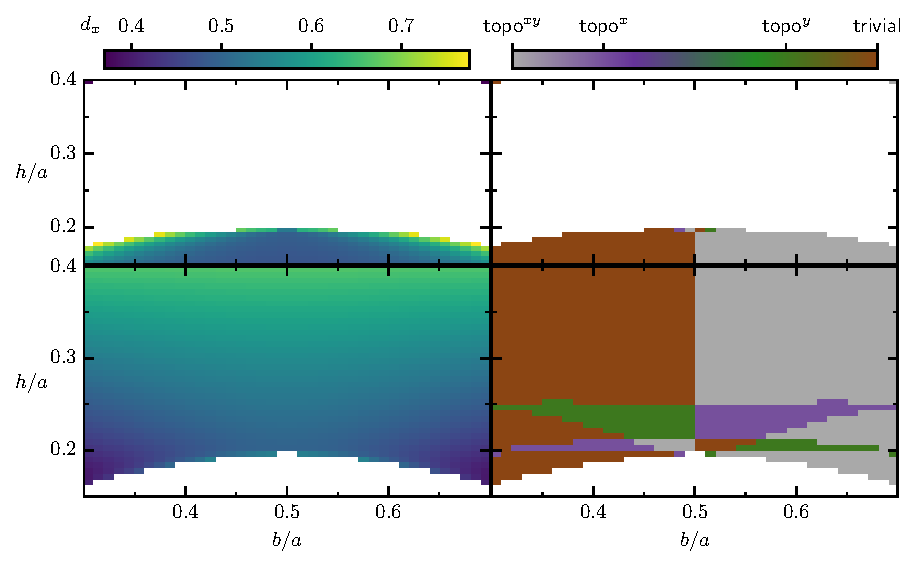
\includegraphics{pictures/topological_phases_decoupled_2D.pdf}
    \caption{\textbf{Topological phase diagram.} There are up to four possible dipole orientations that decouple $x$ and $y$-directions. Two of them are shown on the left panels by depicting the $x$-component of the dipole. White space indicates here that there were no appropriate dipoles found. On the right side of the panel the topological phases are depicted. It is shown, whether a topological phase arises for the $x$, $y$ or both directions, or if the system exhibits a topologically trivial phase.}
    \label{fig:topological phases 1D}
\end{figure}
A different approach to decoupling the two directions of displacement $x$ and $y$, is by choosing different trap frequencies along each direction (see \secref{sec:dipole traps}). If one can still ensure $|\omega_x-\omega_y|\gg|U|\ll\omega_x,\,\omega_y$, the two direction of displacement are decoupled as well, since transfer between the $x$ and $y$-mode are suppressed. In this case one still has free choice over the dipole orientation. Focussing in the following only on one direction, one receives a full one-dimensional model with one mode per site. Eliminating the onsite potential with the help of the trap frequencies, this system can be mapped to an extended SSH-model. The only requirement left for this mapping is the vanishing of interactions within the same sublattice. This can be eliminated by choosing an appropriate dipole orientation, i.e. $d_x=\pm1/\sqrt{3}$.



\chapter*{Spin-phonon coupling}

\section*{Transport}
I want to allow for the propagation of excitations through the chain. The first step towards this is constructing a Hamiltonian which describes the dynamics of a system of Rydberg atoms, where one atom is excited, hence restricting ourselves to the single excitation subspace. The general coupling between the atoms arises from the interaction between the dipole moments of the atoms,
\begin{align*}
    V&=\sum_\mathbf{r}V(\mathbf{r})\\
    \text{with}\quad V(\mathbf{r})&= V_0\,\left(\frac{\mathbf{\hat{d}}_1\cdot\mathbf{\hat{d}}_2}{r^3}-3\,\frac{(\mathbf{r}\cdot \mathbf{\hat{d}}_1)(\mathbf{r}\cdot \mathbf{\hat{d}}_2)}{r^5}\right).
\end{align*}
Each individual atom is characterized by its position in the lattice and its atomic energy level which is captured by the non-interacting Hamiltonian $H_0$. The total Hamiltonian thus reads
\begin{align*}
    H = H_0 + V
\end{align*}
We will investigate the system in a regime, where the coupling due to the dipole forces is much smaller than the energy gap $\Delta$, which separates the energy of the atoms from their next higher and lower states, i.e. $\lVert V \rVert\ll\Delta$. In order to gain an approximate effective Hamiltonian, which acts in a closed way on the one excitation subspace, I will perform a Schrieffer-Wolff transform up to second order \cite{bravyi_schrieffer-wolff_2011}. Let $P_0$ be the projector on the one excitation subspace. Then an exact alternative Hamiltonian $H'$ can be constructed by the transformation
\begin{align*}
    H'&= e^S\,H\,e^{-S}
\end{align*}
for which holds, that it is block-diagonal with respect to the subspaces defined by the projections $P_0$ and $1-P_0$. Thus the alternative Hamiltonian $H'$ is closed with respect to the one excitation subspace and one can define the exact effective Hamiltonian as
\begin{align*}
    H_\text{eff}&=P_0\, e^S\,H\,e^{-S}\,P_0
\end{align*}
Let $\varepsilon$ be of the order of the coupling $\varepsilon=\lVert V \rVert$. The transformation generating operator $S$ can be expanded in orders of $V$.
\begin{align*}
    S&= \sum_{n=1}^\infty \varepsilon^n\,S_n
\end{align*}
I will consider the effective Hamiltonian up to second order in the coupling. This lets $H_\text{eff}$ read
\begin{align*}
    H_\text{eff}&=H_0P_0+P_0VP_0+\frac12\,P_0\,[S_1,V_\text{od}]\,P_0,
\end{align*}
with $V_\text{od}=P_0\,V\,(1-P_0)+(1-P_0)\,V\,P_0$ being the off-diagonal part of the interaction. The first term of the generator $S$ has the form
\begin{align*}
    S_1&=\mathcal{L}(V_\text{od})\\
    \text{with}\quad \mathcal{L}(X)&=\sum_{\substack{i,j\in E\\E_i\neq E_j}}\frac{\braket{i|V|j}}{E_i-E_j}\,\ket{i}\bra{j}
\end{align*}
The sum in the superoperator $\mathcal{L}$ goes over all energy eigenstates, where the $i$, $j$ combination of states with equal energy are omitted. It can be written via a sum over all energies in the single excitations subspace $E1$ and all the other eigenenergies $\tilde{E}$.
\begin{align*}
    \mathcal{L}(X)&=\sum_{\substack{i\in E1\\j\in\tilde{E}}}\frac{\braket{i|V|j}}{E_i-E_j}\,\ket{i}\bra{j}-\text{h.c.}
\end{align*}
From this the commutator term in the effective Hamiltonian can be calculated.
\begin{align*}
    P_0\,[S_1,V_\text{od}]\,P_0&= 2\,\sum_{\substack{i\in E1\\j\in\tilde{E}}}\frac{\left|\braket{i|V|j}\right|^2}{E_i-E_j}\,\ket{i}\bra{i}=\vcentcolon H_{\text{eff},2}
\end{align*}
Thus finally the effective Hamiltonian reads
\begin{align*}
    H_\text{eff}&=H_0P_0+P_0VP_0+\sum_{\substack{i\in E1\\j\in\tilde{E}}}\frac{\left|\braket{i|V|j}\right|^2}{E_i-E_j}\,\ket{i}\bra{i}
\end{align*}
For the effective Hamiltonian the contribution $H_0P_0$ is just a constant term and can be neglected. Further because of the large relative size of $\Delta$ over the interaction strength, I will only include energies into the above sum which differ from the single excitation subspace by $\Delta$. Further the zero excitations subspace does not couple to the one with one excitation in the considered order of expansion. Thus only eigenstates in the double excitation subspace have to be taken into account for the sum.
\begin{figure}[H]
    \centering
    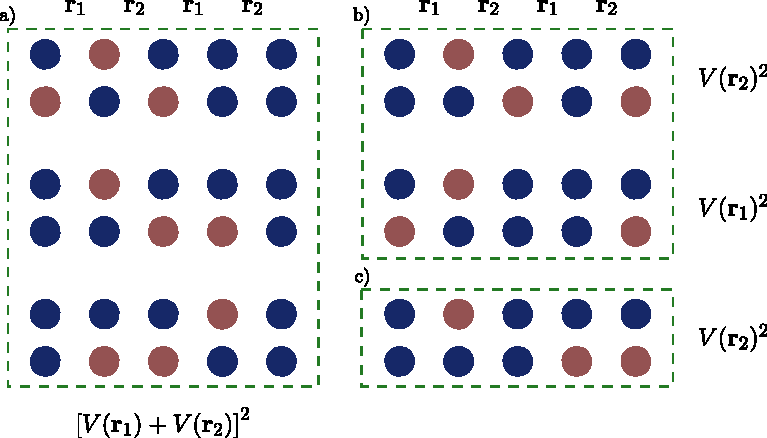
\includegraphics{pictures/SWT_calc.pdf}
    \caption{\textbf{Coupling schemes.} There are different ways double excited states couple to the single excited ones. The top row always depicts a state of the single, while the bottom row depicts a state of the double excited subspace. Generally configurations of two different subspaces are coupled to each other, when for two neighboring atoms one configuration has the inverted excitation scheme with respect to the other. I assign them to three categories. The first category is depicted in a). It couples two neighboring atoms twice. In the picture all possible cases are shown. For b) only two atoms couple two each other. Here the coupling takes place at a pair of $\ket{e}$ and $\ket{g}$ in both configurations. If the excitation in the single excitation subspace is at position $2<i<N-1$, there are $N-4$ different states in the double excited subspace that contribute a term $V(\mathbf{r}_1)^2$ and the same number for $V(\mathbf{r}_2)^2$. Category c) couples two unexcited sites in the single excitations subspace to two excited sites in the double excited subspace. For this case there are $N/2-2$ states that contribute $V(\mathbf{r}_1)^2$ and  $N/2-2$ states that contribute $V(\mathbf{r}_2)^2$, if the single excited state is is excited at atom $2<i<N-1$.}
    \label{fig:SWT_schemes}
\end{figure}
In the following the effective Hamiltonian will be calculated for the specific configuration we are looking at. We consider a one-dimensional staggered chain of $N$ atoms, where the atoms are separated by alternating distances $\mathbf{r}_1$ and $\mathbf{r}_2$. For a single atom there are only two states available, excited $\ket{e}$ and unexcited $\ket{g}$. The states $\ket{i}$, which are summed over, represent the states where only atom $i$ is excited and the others are in the unexcited state. Going to a regime where only nearest neighbor interactions contribute we can write using the coupling schemes of \figref{fig:SWT_schemes}
\begin{align*}
    H_{\text{eff},2}&= \sum_{i=1}^N\tilde{V}_i\,\ket{i}\bra{i}\\
    \tilde{V}_i &=-\frac{1}{\Delta}\,\begin{cases}
        3\,\left[V(\mathbf{r}_1)+V(\mathbf{r}_2)\right]^2+(N-4+\frac{N}{2}-2)\,V^2(\mathbf{r}_1)+(N-4+\frac{N}{2}-2)\,V^2(\mathbf{r}_2)&\text{if}\;1\neq i\neq N\\\\
        \left[V(\mathbf{r}_1)+V(\mathbf{r}_2)\right]^2+(N-3+\frac{N}{2}-1)\,V^2(\mathbf{r}_1)+(\frac{N}{2}-1)\,V^2(\mathbf{r}_2)&\text{if}\;i=1\\\\
        2\,\left[V(\mathbf{r}_1)+V(\mathbf{r}_2)\right]^2+(N-3+\frac{N}{2}-2)\,V^2(\mathbf{r}_1)+(N-4+\frac{N}{2}-1)\,V^2(\mathbf{r}_2)&\text{if}\;i=2\\\\
        2\,\left[V(\mathbf{r}_1)+V(\mathbf{r}_2)\right]^2+(N-4+\frac{N}{2}-1)\,V^2(\mathbf{r}_1)+(N-3+\frac{N}{2}-2)\,V^2(\mathbf{r}_2)&\text{if}\;i=N-1\\\\
        \left[V(\mathbf{r}_1)+V(\mathbf{r}_2)\right]^2+(\frac{N}{2}-1)\,V^2(\mathbf{r}_1)+(N-3+\frac{N}{2}-1)\,V^2(\mathbf{r}_2)&\text{if}\;i=N
    \end{cases}
\end{align*}
% There is actually another case distinction necessary for $i=2$ and $i=N-1$, this will be clearer later.
The part involving interactions within the same subspace can be written as 
\begin{align*}
    P_0VP_0&= \sum_{\substack{i=1\\j=i+1}}^{N-1} V(\mathbf{r}_{i,j})\,\sigma^+_i\sigma^-_j+\text{h.c.},
\end{align*}
where $\mathbf{r}_{i,j}$ is the distance between the $i$th and $j$th site. I now also want to write $H_{\text{eff},2}$ in terms of a sum of two atom operators. Therefore I introduce the projectors $n^e_i=\ket{e}_i\bra{e}_i$ and $n^g_i=\ket{g}_i\bra{g}_i$.
\begin{align*}
    H_{\text{eff},2}&=\sum_{\substack{i=1\\j=i+1}}^{N-1}V^2(\mathbf{r}_{i,j})\,(n^e_in^g_j + n^g_in^e_j + n^g_in^g_j)+\sum_{i=2}^{N-1}\left[ V(\mathbf{r}_{i-1,i})+V(\mathbf{r}_{i,i+1}) \right]^2 \, n^g_{i-1}n^e_in^g_{i+1}\\ &+\sum_{i=3}^{N-1} \left[ V(\mathbf{r}_{i-2,i-1})+V(\mathbf{r}_{i-1,i}) \right]^2 \, n^g_{i-2}n^g_{i-1}n^e_{i} 
    +\sum_{i=2}^{N-2} \left[ V(\mathbf{r}_{i,i+1})+V(\mathbf{r}_{i+1,i+2}) \right]^2 \, n^e_{i}n^g_{i+1}n^g_{i+2} \\
    &+ \left[ V(\mathbf{r}_{1,2})+V(\mathbf{r}_{2,3}) \right]^2 n^e_1n^g_2n^g_3 + \left[ V(\mathbf{r}_{N-2,N-1})+V(\mathbf{r}_{N-1,N}) \right]^2 n^g_{N-2}n^g_{N-1}n^e_{N}
\end{align*}
A last step is possible since in the single excitation subspace terms like $n^e_in^g_j$ simplify to just $n^e_i$.
\begin{align*}
    &= \sum_{i=2}^{N-1}\left(V^2(\mathbf{r}_{i-1,i})+V^2(\mathbf{r}_{i,i+1})+\left[ V(\mathbf{r}_{i-1,i})+V(\mathbf{r}_{i,i+1}) \right]^2 \right)\,n^e_i \\&+ \sum_{i=3}^{N-1} \left[ V(\mathbf{r}_{i-2,i-1})+V(\mathbf{r}_{i-1,i}) \right]^2\, n^e_i +\sum_{i=2}^{N-2} \left[ V(\mathbf{r}_{i,i+1})+V(\mathbf{r}_{i+1,i+2}) \right]^2\,n^e_i\\
    &+ \left( V^2(\mathbf{r}_{1,2}) + \left[ V(\mathbf{r}_{1,2})+V(\mathbf{r}_{2,3}) \right]^2 \right)\,n^e_1 + \left( V^2(\mathbf{r}_{N-1,N})+ \left[ V(\mathbf{r}_{N-2,N-1})+V(\mathbf{r}_{N-1,N}) \right]^2\right)\,n^e_N\\
    &+ \sum_{i=1}^{N-1} V(\mathbf{r}_{i,i+1})\,n^g_in^g_{i+1}
\end{align*}
\subsection*{Energy scales}
The most important energies which determine the dynamics are the trap frequency, which is of the order $\omega\sim10\,\text{-}\,100\,\text{kHz}$, the distances between atoms who can reliably reach $3\,\mu\text{m}$, and the lifetime of the Rydberg states, which is in the order of $100\,\mu\text{s}$. From this it already becomes apparent that, in order to see dynamics of the system within the lifetime of the Rydberg states, the coupling strength has to be higher than the trap frequency. This prevents the Lamb-Dicke regime, as the phonon number cannot be assumed as conserved. Thus the first order expansion in the deplacements of the atoms has to be taken into account. The relative size of each order of the expansion can be estimated by the factor
\begin{align*}
    \varepsilon\vcentcolon=\sqrt{\frac{\hbar}{m\omega}}\,\frac1r\approx(2\,\text{-}\,11)\cdot10^{-3}
\end{align*}
As the dipole interaction is a function of the angle $\vartheta$ between the dipole moment and the axis of the chain, the interaction can be tuned in a way that the first order term vanishes. As can be seen in \figref{fig:dipole_orientation_for_vanishing_first_order}, the second order term in the expansion is of the order $5\cdot10^{-5}\,\text{-}\,10^{-3}$, smaller than the leading order. 
\begin{figure}[H]
    \centering
    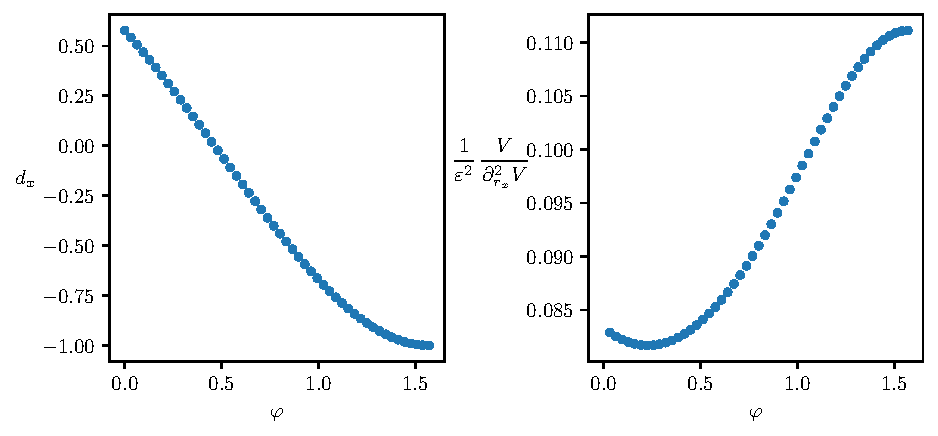
\includegraphics{pictures/magnitude_dersqV_ifderVzero.pdf}
    \caption{\textbf{Dipole orientation and ratio of interactions.} For all angles $\sin\varphi\vcentcolon=h/r$ one can find a dipole orientation, shown in the left panel, such thatthe first order term in the expansion of the interaction vanishes. The ratio between zeroth order and second order term is shown in the right panel. }
    \label{fig:dipole_orientation_for_vanishing_first_order}
\end{figure}




\subsection*{First order approximation in spin degrees}
For the first approach I will continue with the Hamiltonian up to first order in the dipole interaction, i.e. without $H_{\text{eff},2}$. The phonons are introduced by again expanding the interaction up to second order. When we choose the dipole orientation, such that thr first order vanishes, the Hamiltonian reads
\begin{align*}
    H&= \sum_{i=1}^{N-1}\left[V(\mathbf{r}_{i,i+1})+\frac12\,\sum_{n,m\in\{i,i+1\}}\frac{\partial^2V(\mathbf{r}_{i,i+1})}{\partial\mathbf{r}_{n}\partial\mathbf{r}_m}\,\delta\mathbf{\hat{r}}_n\delta\mathbf{\hat{r}}_m\right]\,\sigma_i^+\sigma_{i+1}^-+\text{h.c.}\\
    &= \sum_{i=1}^{N-1}\left[V(\mathbf{r}_{i,i+1})-\frac{\hbar}{2m\omega}\,\frac{\partial^2V(\mathbf{r}_{i,i+1})}{\partial\mathbf{r}_{i}^2}\,\left(p_j^\dagger p_{j+1}+p_{j+1}^\dagger p_{j}-p_{j}^\dagger p_{j}-p_{j+1}^\dagger p_{j+1}\right)\right]\,\sigma_i^+\sigma_{i+1}^-+\text{h.c.}
\end{align*}
The quadrature operators of the phonons are used $\delta\mathbf{\hat{r}}_i=\sqrt{\frac{\hbar}{2m\omega}}\,(p_i + p_i^\dagger)$. In the following I want to present a brief investigation of the influence of this small second order term on the dynamics of the spins. Ultimately I am interested in the effect of the phonons on the transport of spin excitations via a Rice-Mele scheme. Therefore I will compare the free evolution of the system with and without phonons at conditions mimicking a point in the middle of the Rice-Mele cycle, where the dynamics are the fastest. The results are shown in \figref{fig:diff_free_evol_with_without_phonons}. As can be seen, for high phonon excitation numbers the difference in the spin excitations during the time period of the whole cycle becomes substantial. Nevertheless, the performance of the Rice-Mele protocol is affected only mildly, and is even slightly improved by the inclusion of the phonons, as can be seen in \figref{fig:end_excitation_rice_mele_with_without_phonons}.

\begin{figure}[H]
    \hspace*{-1.5cm}
    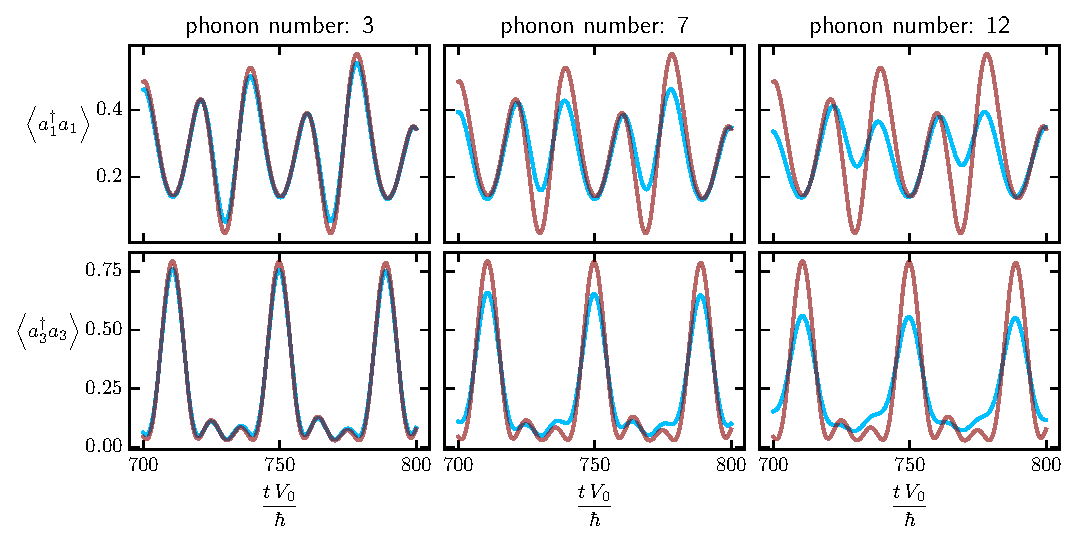
\includegraphics{pictures/compare_with_without_phonon_late_time.pdf}
    \caption{\textbf{Comparison of free evolution with and without phonons.} The difference in spin excitation probability between the free evolution with and without phonons is shown for a chain of length $N=4$. As initial conditions I chose a quadratically decaying excitation profile from the right edge and parameters $b=1.2\,r_0$, $h=0.4\,r_0$, $a=3\,r_0$. The red line shows the trajectory for the case without motional degrees of freedom and the blue one the case with phonons present.For an atom with 12 motional excitations the mean displacement is of the order of $0.15\,\mu\text{m}$, which is already around the limit of the expansion to second order being accurate.}
    \label{fig:diff_free_evol_with_without_phonons}
\end{figure}

\begin{figure}[H]
    \hspace*{-1.5cm}
    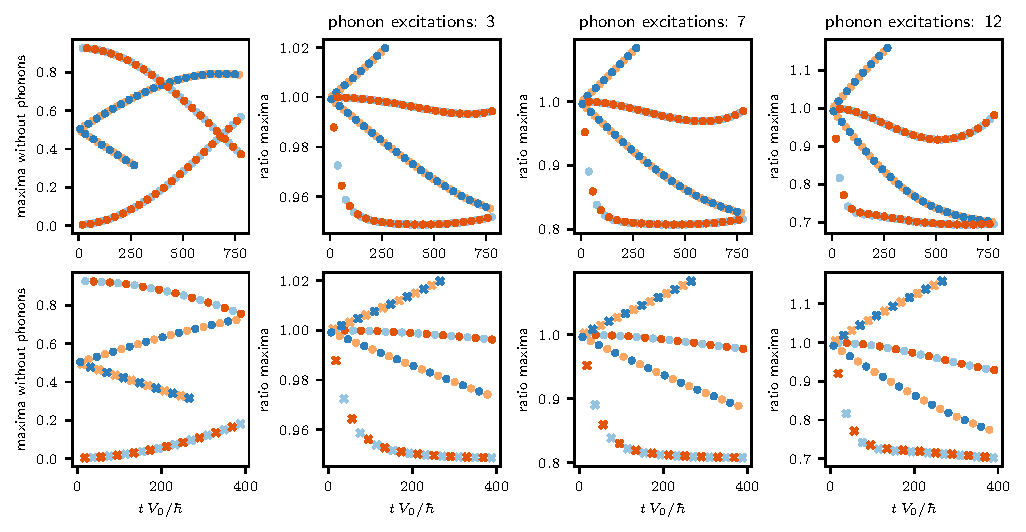
\includegraphics{pictures/maxima_compared_free_evolution.pdf}
    \caption{\textbf{Comparison of the maxima of the free evolution with and without phonons.} For the same parameters and initial conditions as in \figref{fig:diff_free_evol_with_without_phonons} the maxima of the spin excitation probability at the individual sites are compared for the free evolution with and without phonons. }
    % \label{fig:diff_free_evol_with_without_phonons}
\end{figure}

\begin{figure}[H]
    \centering
    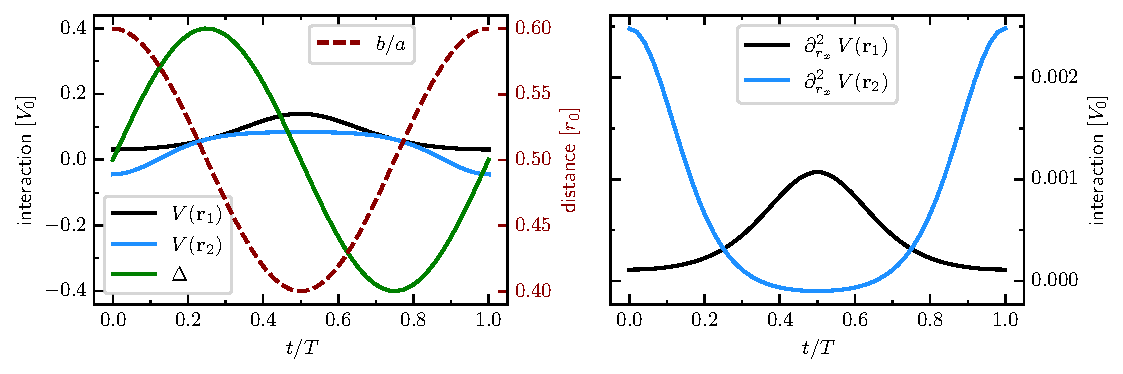
\includegraphics{pictures/rice-mele-scheme1to1000.pdf}
    \caption{\textbf{Rice-Mele scheme.} Depicted is the course of the the decisive parameters during the Rice-Mele cycle, i.e. the axial distance between atoms in the unit cell $b=1.8\,\text{-}\,1.2\,\text{-}\,1.8\,r_0$ (the distance orthogonal to the chain axis is kept constant $h=0.4\,r_0$ as well as the distance inside a sublattice $a=3\,r_0$). The detuning takes it's maximal value at $\Delta_\text{max}=0.4\,V_0$.}
    % \label{fig:end_excitation_rice_mele_with_without_phonons}
\end{figure}

\begin{figure}[H]
    \centering
    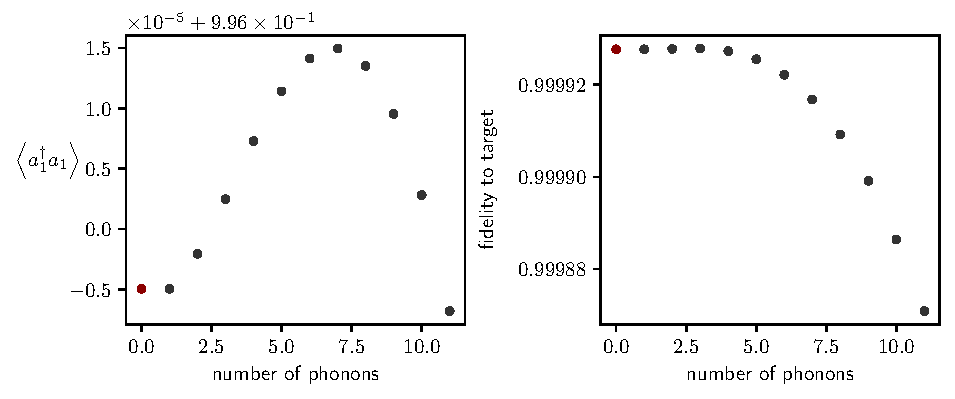
\includegraphics{pictures/transfered_excitation_depphon.pdf}
    \caption{\textbf{Transfered excitation in dependence of phonon number.} I show the excitation probability at the left edge at the end of the cycle, when the system is initialized in an eigenstate of the pure spin Hamiltonian localized at the right edge. And parameters of the cycle are $b=1.8\,\text{-}\,1.2\,\text{-}\,1.8\,r_0$, $h=0.4\,r_0$, $a=3\,r_0$, $\Delta_\text{max}=0.4\,V_0$.}
    \label{fig:end_excitation_rice_mele_with_without_phonons}
\end{figure}
% \chapter*{Spin-phonon coupling}

\section*{Transport}
I want to allow for the propagation of excitations through the chain. The first step towards this is constructing a Hamiltonian which describes the dynamics of a system of Rydberg atoms, where one atom is excited, hence restricting ourselves to the single excitation subspace. The general coupling between the atoms arises from the interaction between the dipole moments of the atoms,
\begin{align*}
    V&=\sum_\mathbf{r}V(\mathbf{r})\\
    \text{with}\quad V(\mathbf{r})&= V_0\,\left(\frac{\mathbf{\hat{d}}_1\cdot\mathbf{\hat{d}}_2}{r^3}-3\,\frac{(\mathbf{r}\cdot \mathbf{\hat{d}}_1)(\mathbf{r}\cdot \mathbf{\hat{d}}_2)}{r^5}\right).
\end{align*}
Each individual atom is characterized by its position in the lattice and its atomic energy level which is captured by the non-interacting Hamiltonian $H_0$. The total Hamiltonian thus reads
\begin{align*}
    H = H_0 + V
\end{align*}
We will investigate the system in a regime, where the coupling due to the dipole forces is much smaller than the energy gap $\Delta$, which separates the energy of the atoms from their next higher and lower states, i.e. $\lVert V \rVert\ll\Delta$. In order to gain an approximate effective Hamiltonian, which acts in a closed way on the one excitation subspace, I will perform a Schrieffer-Wolff transform up to second order \cite{bravyi_schrieffer-wolff_2011}. Let $P_0$ be the projector on the one excitation subspace. Then an exact alternative Hamiltonian $H'$ can be constructed by the transformation
\begin{align*}
    H'&= e^S\,H\,e^{-S}
\end{align*}
for which holds, that it is block-diagonal with respect to the subspaces defined by the projections $P_0$ and $1-P_0$. Thus the alternative Hamiltonian $H'$ is closed with respect to the one excitation subspace and one can define the exact effective Hamiltonian as
\begin{align*}
    H_\text{eff}&=P_0\, e^S\,H\,e^{-S}\,P_0
\end{align*}
Let $\varepsilon$ be of the order of the coupling $\varepsilon=\lVert V \rVert$. The transformation generating operator $S$ can be expanded in orders of $V$.
\begin{align*}
    S&= \sum_{n=1}^\infty \varepsilon^n\,S_n
\end{align*}
I will consider the effective Hamiltonian up to second order in the coupling. This lets $H_\text{eff}$ read
\begin{align*}
    H_\text{eff}&=H_0P_0+P_0VP_0+\frac12\,P_0\,[S_1,V_\text{od}]\,P_0,
\end{align*}
with $V_\text{od}=P_0\,V\,(1-P_0)+(1-P_0)\,V\,P_0$ being the off-diagonal part of the interaction. The first term of the generator $S$ has the form
\begin{align*}
    S_1&=\mathcal{L}(V_\text{od})\\
    \text{with}\quad \mathcal{L}(X)&=\sum_{\substack{i,j\in E\\E_i\neq E_j}}\frac{\braket{i|V|j}}{E_i-E_j}\,\ket{i}\bra{j}
\end{align*}
The sum in the superoperator $\mathcal{L}$ goes over all energy eigenstates, where the $i$, $j$ combination of states with equal energy are omitted. It can be written via a sum over all energies in the single excitations subspace $E1$ and all the other eigenenergies $\tilde{E}$.
\begin{align*}
    \mathcal{L}(X)&=\sum_{\substack{i\in E1\\j\in\tilde{E}}}\frac{\braket{i|V|j}}{E_i-E_j}\,\ket{i}\bra{j}-\text{h.c.}
\end{align*}
From this the commutator term in the effective Hamiltonian can be calculated.
\begin{align*}
    P_0\,[S_1,V_\text{od}]\,P_0&= 2\,\sum_{\substack{i\in E1\\j\in\tilde{E}}}\frac{\left|\braket{i|V|j}\right|^2}{E_i-E_j}\,\ket{i}\bra{i}=\vcentcolon H_{\text{eff},2}
\end{align*}
Thus finally the effective Hamiltonian reads
\begin{align*}
    H_\text{eff}&=H_0P_0+P_0VP_0+\sum_{\substack{i\in E1\\j\in\tilde{E}}}\frac{\left|\braket{i|V|j}\right|^2}{E_i-E_j}\,\ket{i}\bra{i}
\end{align*}
For the effective Hamiltonian the contribution $H_0P_0$ is just a constant term and can be neglected. Further because of the large relative size of $\Delta$ over the interaction strength, I will only include energies into the above sum which differ from the single excitation subspace by $\Delta$. Further the zero excitations subspace does not couple to the one with one excitation in the considered order of expansion. Thus only eigenstates in the double excitation subspace have to be taken into account for the sum.
\begin{figure}[H]
    \centering
    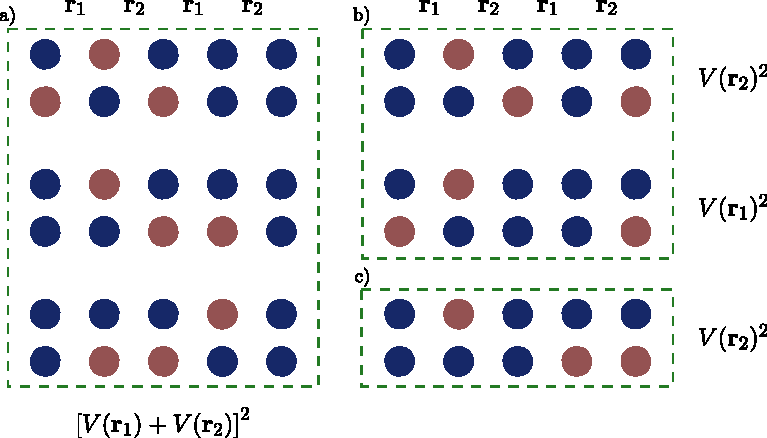
\includegraphics{pictures/SWT_calc.pdf}
    \caption{\textbf{Coupling schemes.} There are different ways double excited states couple to the single excited ones. The top row always depicts a state of the single, while the bottom row depicts a state of the double excited subspace. Generally configurations of two different subspaces are coupled to each other, when for two neighboring atoms one configuration has the inverted excitation scheme with respect to the other. I assign them to three categories. The first category is depicted in a). It couples two neighboring atoms twice. In the picture all possible cases are shown. For b) only two atoms couple two each other. Here the coupling takes place at a pair of $\ket{e}$ and $\ket{g}$ in both configurations. If the excitation in the single excitation subspace is at position $2<i<N-1$, there are $N-4$ different states in the double excited subspace that contribute a term $V(\mathbf{r}_1)^2$ and the same number for $V(\mathbf{r}_2)^2$. Category c) couples two unexcited sites in the single excitations subspace to two excited sites in the double excited subspace. For this case there are $N/2-2$ states that contribute $V(\mathbf{r}_1)^2$ and  $N/2-2$ states that contribute $V(\mathbf{r}_2)^2$, if the single excited state is is excited at atom $2<i<N-1$.}
    \label{fig:SWT_schemes}
\end{figure}
In the following the effective Hamiltonian will be calculated for the specific configuration we are looking at. We consider a one-dimensional staggered chain of $N$ atoms, where the atoms are separated by alternating distances $\mathbf{r}_1$ and $\mathbf{r}_2$. For a single atom there are only two states available, excited $\ket{e}$ and unexcited $\ket{g}$. The states $\ket{i}$, which are summed over, represent the states where only atom $i$ is excited and the others are in the unexcited state. Going to a regime where only nearest neighbor interactions contribute we can write using the coupling schemes of \figref{fig:SWT_schemes}
\begin{align*}
    H_{\text{eff},2}&= \sum_{i=1}^N\tilde{V}_i\,\ket{i}\bra{i}\\
    \tilde{V}_i &=-\frac{1}{\Delta}\,\begin{cases}
        3\,\left[V(\mathbf{r}_1)+V(\mathbf{r}_2)\right]^2+(N-4+\frac{N}{2}-2)\,V^2(\mathbf{r}_1)+(N-4+\frac{N}{2}-2)\,V^2(\mathbf{r}_2)&\text{if}\;1\neq i\neq N\\\\
        \left[V(\mathbf{r}_1)+V(\mathbf{r}_2)\right]^2+(N-3+\frac{N}{2}-1)\,V^2(\mathbf{r}_1)+(\frac{N}{2}-1)\,V^2(\mathbf{r}_2)&\text{if}\;i=1\\\\
        2\,\left[V(\mathbf{r}_1)+V(\mathbf{r}_2)\right]^2+(N-3+\frac{N}{2}-2)\,V^2(\mathbf{r}_1)+(N-4+\frac{N}{2}-1)\,V^2(\mathbf{r}_2)&\text{if}\;i=2\\\\
        2\,\left[V(\mathbf{r}_1)+V(\mathbf{r}_2)\right]^2+(N-4+\frac{N}{2}-1)\,V^2(\mathbf{r}_1)+(N-3+\frac{N}{2}-2)\,V^2(\mathbf{r}_2)&\text{if}\;i=N-1\\\\
        \left[V(\mathbf{r}_1)+V(\mathbf{r}_2)\right]^2+(\frac{N}{2}-1)\,V^2(\mathbf{r}_1)+(N-3+\frac{N}{2}-1)\,V^2(\mathbf{r}_2)&\text{if}\;i=N
    \end{cases}
\end{align*}
% There is actually another case distinction necessary for $i=2$ and $i=N-1$, this will be clearer later.
The part involving interactions within the same subspace can be written as 
\begin{align*}
    P_0VP_0&= \sum_{\substack{i=1\\j=i+1}}^{N-1} V(\mathbf{r}_{i,j})\,\sigma^+_i\sigma^-_j+\text{h.c.},
\end{align*}
where $\mathbf{r}_{i,j}$ is the distance between the $i$th and $j$th site. I now also want to write $H_{\text{eff},2}$ in terms of a sum of two atom operators. Therefore I introduce the projectors $n^e_i=\ket{e}_i\bra{e}_i$ and $n^g_i=\ket{g}_i\bra{g}_i$.
\begin{align*}
    H_{\text{eff},2}&=\sum_{\substack{i=1\\j=i+1}}^{N-1}V^2(\mathbf{r}_{i,j})\,(n^e_in^g_j + n^g_in^e_j + n^g_in^g_j)+\sum_{i=2}^{N-1}\left[ V(\mathbf{r}_{i-1,i})+V(\mathbf{r}_{i,i+1}) \right]^2 \, n^g_{i-1}n^e_in^g_{i+1}\\ &+\sum_{i=3}^{N-1} \left[ V(\mathbf{r}_{i-2,i-1})+V(\mathbf{r}_{i-1,i}) \right]^2 \, n^g_{i-2}n^g_{i-1}n^e_{i} 
    +\sum_{i=2}^{N-2} \left[ V(\mathbf{r}_{i,i+1})+V(\mathbf{r}_{i+1,i+2}) \right]^2 \, n^e_{i}n^g_{i+1}n^g_{i+2} \\
    &+ \left[ V(\mathbf{r}_{1,2})+V(\mathbf{r}_{2,3}) \right]^2 n^e_1n^g_2n^g_3 + \left[ V(\mathbf{r}_{N-2,N-1})+V(\mathbf{r}_{N-1,N}) \right]^2 n^g_{N-2}n^g_{N-1}n^e_{N}
\end{align*}
A last step is possible since in the single excitation subspace terms like $n^e_in^g_j$ simplify to just $n^e_i$.
\begin{align*}
    &= \sum_{i=2}^{N-1}\left(V^2(\mathbf{r}_{i-1,i})+V^2(\mathbf{r}_{i,i+1})+\left[ V(\mathbf{r}_{i-1,i})+V(\mathbf{r}_{i,i+1}) \right]^2 \right)\,n^e_i \\&+ \sum_{i=3}^{N-1} \left[ V(\mathbf{r}_{i-2,i-1})+V(\mathbf{r}_{i-1,i}) \right]^2\, n^e_i +\sum_{i=2}^{N-2} \left[ V(\mathbf{r}_{i,i+1})+V(\mathbf{r}_{i+1,i+2}) \right]^2\,n^e_i\\
    &+ \left( V^2(\mathbf{r}_{1,2}) + \left[ V(\mathbf{r}_{1,2})+V(\mathbf{r}_{2,3}) \right]^2 \right)\,n^e_1 + \left( V^2(\mathbf{r}_{N-1,N})+ \left[ V(\mathbf{r}_{N-2,N-1})+V(\mathbf{r}_{N-1,N}) \right]^2\right)\,n^e_N\\
    &+ \sum_{i=1}^{N-1} V(\mathbf{r}_{i,i+1})\,n^g_in^g_{i+1}
\end{align*}
\subsection*{First order approximation}
For the first approach I will continue with the Hamiltonian up to first order in the dipole interaction, i.e. without $H_{\text{eff},2}$. The phonons are introduced by again expanding the interaction up to second order. I will restrict the consideration also to the constant phonon excitation subspace. For this reason the first order expansion of the dipole interaction will be ignored, as it couples subspaces with different phonon numbers. The Hamiltonian thus reads
\begin{align*}
    H&= \sum_{i=1}^{N-1}\left[V(\mathbf{r}_{i,i+1})+\sum_{n,m\in\{i,i+1\}}\frac{\partial^2V(\mathbf{r}_{i,i+1})}{\partial\mathbf{r}_{n}\partial\mathbf{r}_m}\,\delta\mathbf{\hat{r}}_n\delta\mathbf{\hat{r}}_m\right]\,\sigma_i^+\sigma_{i+1}^-+\text{h.c.}
\end{align*}
The hats in $\delta\mathbf{\hat{r}}$ indicates operators. Here also the operators are projected on the constant phonon subspace. What has to be accounted for is that this second order expansion is only valid if the displacement is small, which means $1/\sqrt{m\omega}\ll1$ as $||a||\sim1$.
\begin{align*}
    \left| 1- \frac{V(\mathbf{r}+\delta\mathbf{r})}{V(\mathbf{r})} \right|&\ll 1\\
    \left| \frac{\partial^2 V(\mathbf{r})}{\partial\mathbf{r}^2}\,\delta\mathbf{r}^2 \right|&\ll\left|V(\mathbf{r})\right|
\end{align*}
When quantizing the displacements to phonon operators $\delta\mathbf{r}^2\rightarrow \frac{2}{m\omega}\,a^\dagger a$, one finds the condition 
\begin{align*}
    \frac{2}{m\omega}\, \left| \frac{\partial^2 V(\mathbf{r})}{\partial\mathbf{r}^2} \right|&\ll\left|V(\mathbf{r})\right|,
\end{align*}
as $a^\dagger a$ is of the order of 1. 
\begin{figure}[H]
    \centering
    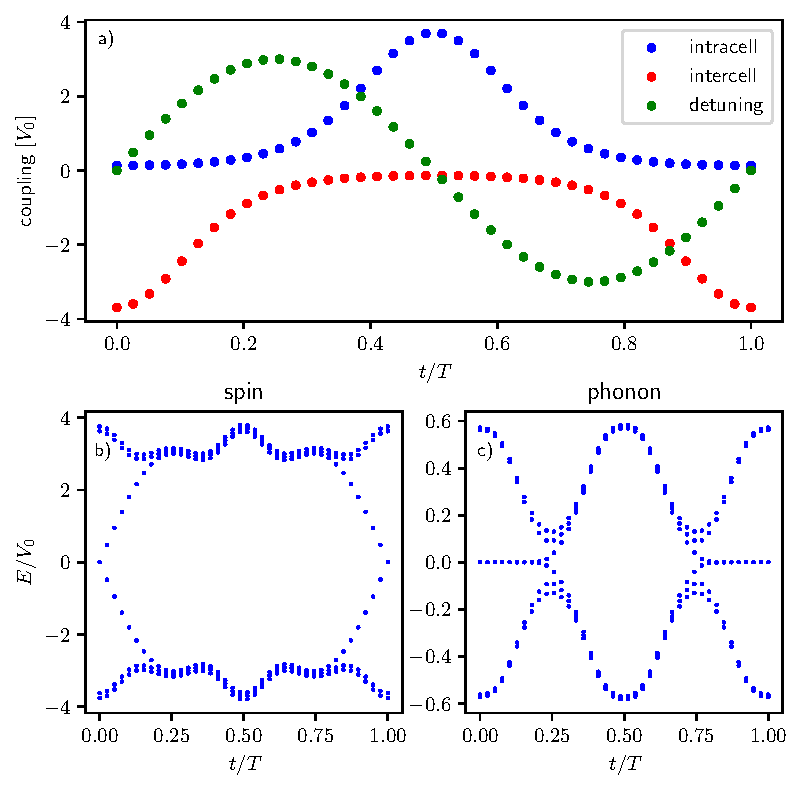
\includegraphics{pictures/rice_mele_protocol.pdf}
    \caption{\textbf{Spin transfer protocol.} In a the course of the interaction during the transfer protocol is shown. b-c show the spectrum of the spin and phonon Hamiltonian respectively during the pump cycle each for one excitation in the respective degrees of freedom. For the spin Hamiltonian a pure dipole dipole interaction is used, where the dipole moments of the atoms are orientated in way that puts the interactions within the same sublattice to zero. This choice improves the accuracy of the nearest neighbor assumption. The phonon spectrum is received by the methods used in the previous chapters. It therefore depicts a scenario without spin degrees of freedom.}
    \label{fig:pump_protocol}
\end{figure}
As a next step I want to first discard the phonon dynamics and realize a transfer protocol for a spin excitation through the chain. For this purpose I implement a Rice-Mele model configuration for the chain of Rydberg atoms. This is achieved by including an onsite potential with alternating sign of the form
\begin{align*}
    H_\text{OS}= \sum_{i=1}^N(-1)^i \,\Delta\,\sigma^+_i\sigma^-_i.
\end{align*}
Note that the detuning $\Delta$ is now a different parameter from above. By changing the position and detuning in an adiabatic cyclic way, one can implement a transfer protocol, which is depicted in \figref{fig:pump_protocol}. The system is initialized with the eigenstate of the spin Hamiltonian located at the edge. This is possible, as I start the transfer protocol in the topological phase. After the the transfer period I compare the evolved state with the target state, which is the eigenstate located at the other side. I use a chain of six atoms in total. The resulting fidelity between final and target state for this protocol is $0.9996$.\\\\
I can now compare which influence the introduction of photons has on the transfer quality. Therefore I test the effect of four different phonon initial states on the transfer process. The different initial phonon states can be read of \figref{fig:transfer_trajectories}. \figref{fig:fidelity} shows that the evolvement of the phonon degrees of freedom does not change the quality of the transfer to a very considerable portion, where I investigated how the strength of the phonon-phonon interactions effect
the fidelity of final and target state. In \figref{fig:2phonon_exc_traj} I show the time evolution of the phononic degrees of freedom for two initial phonon excitations.


\begin{figure}[H]
    \centering
    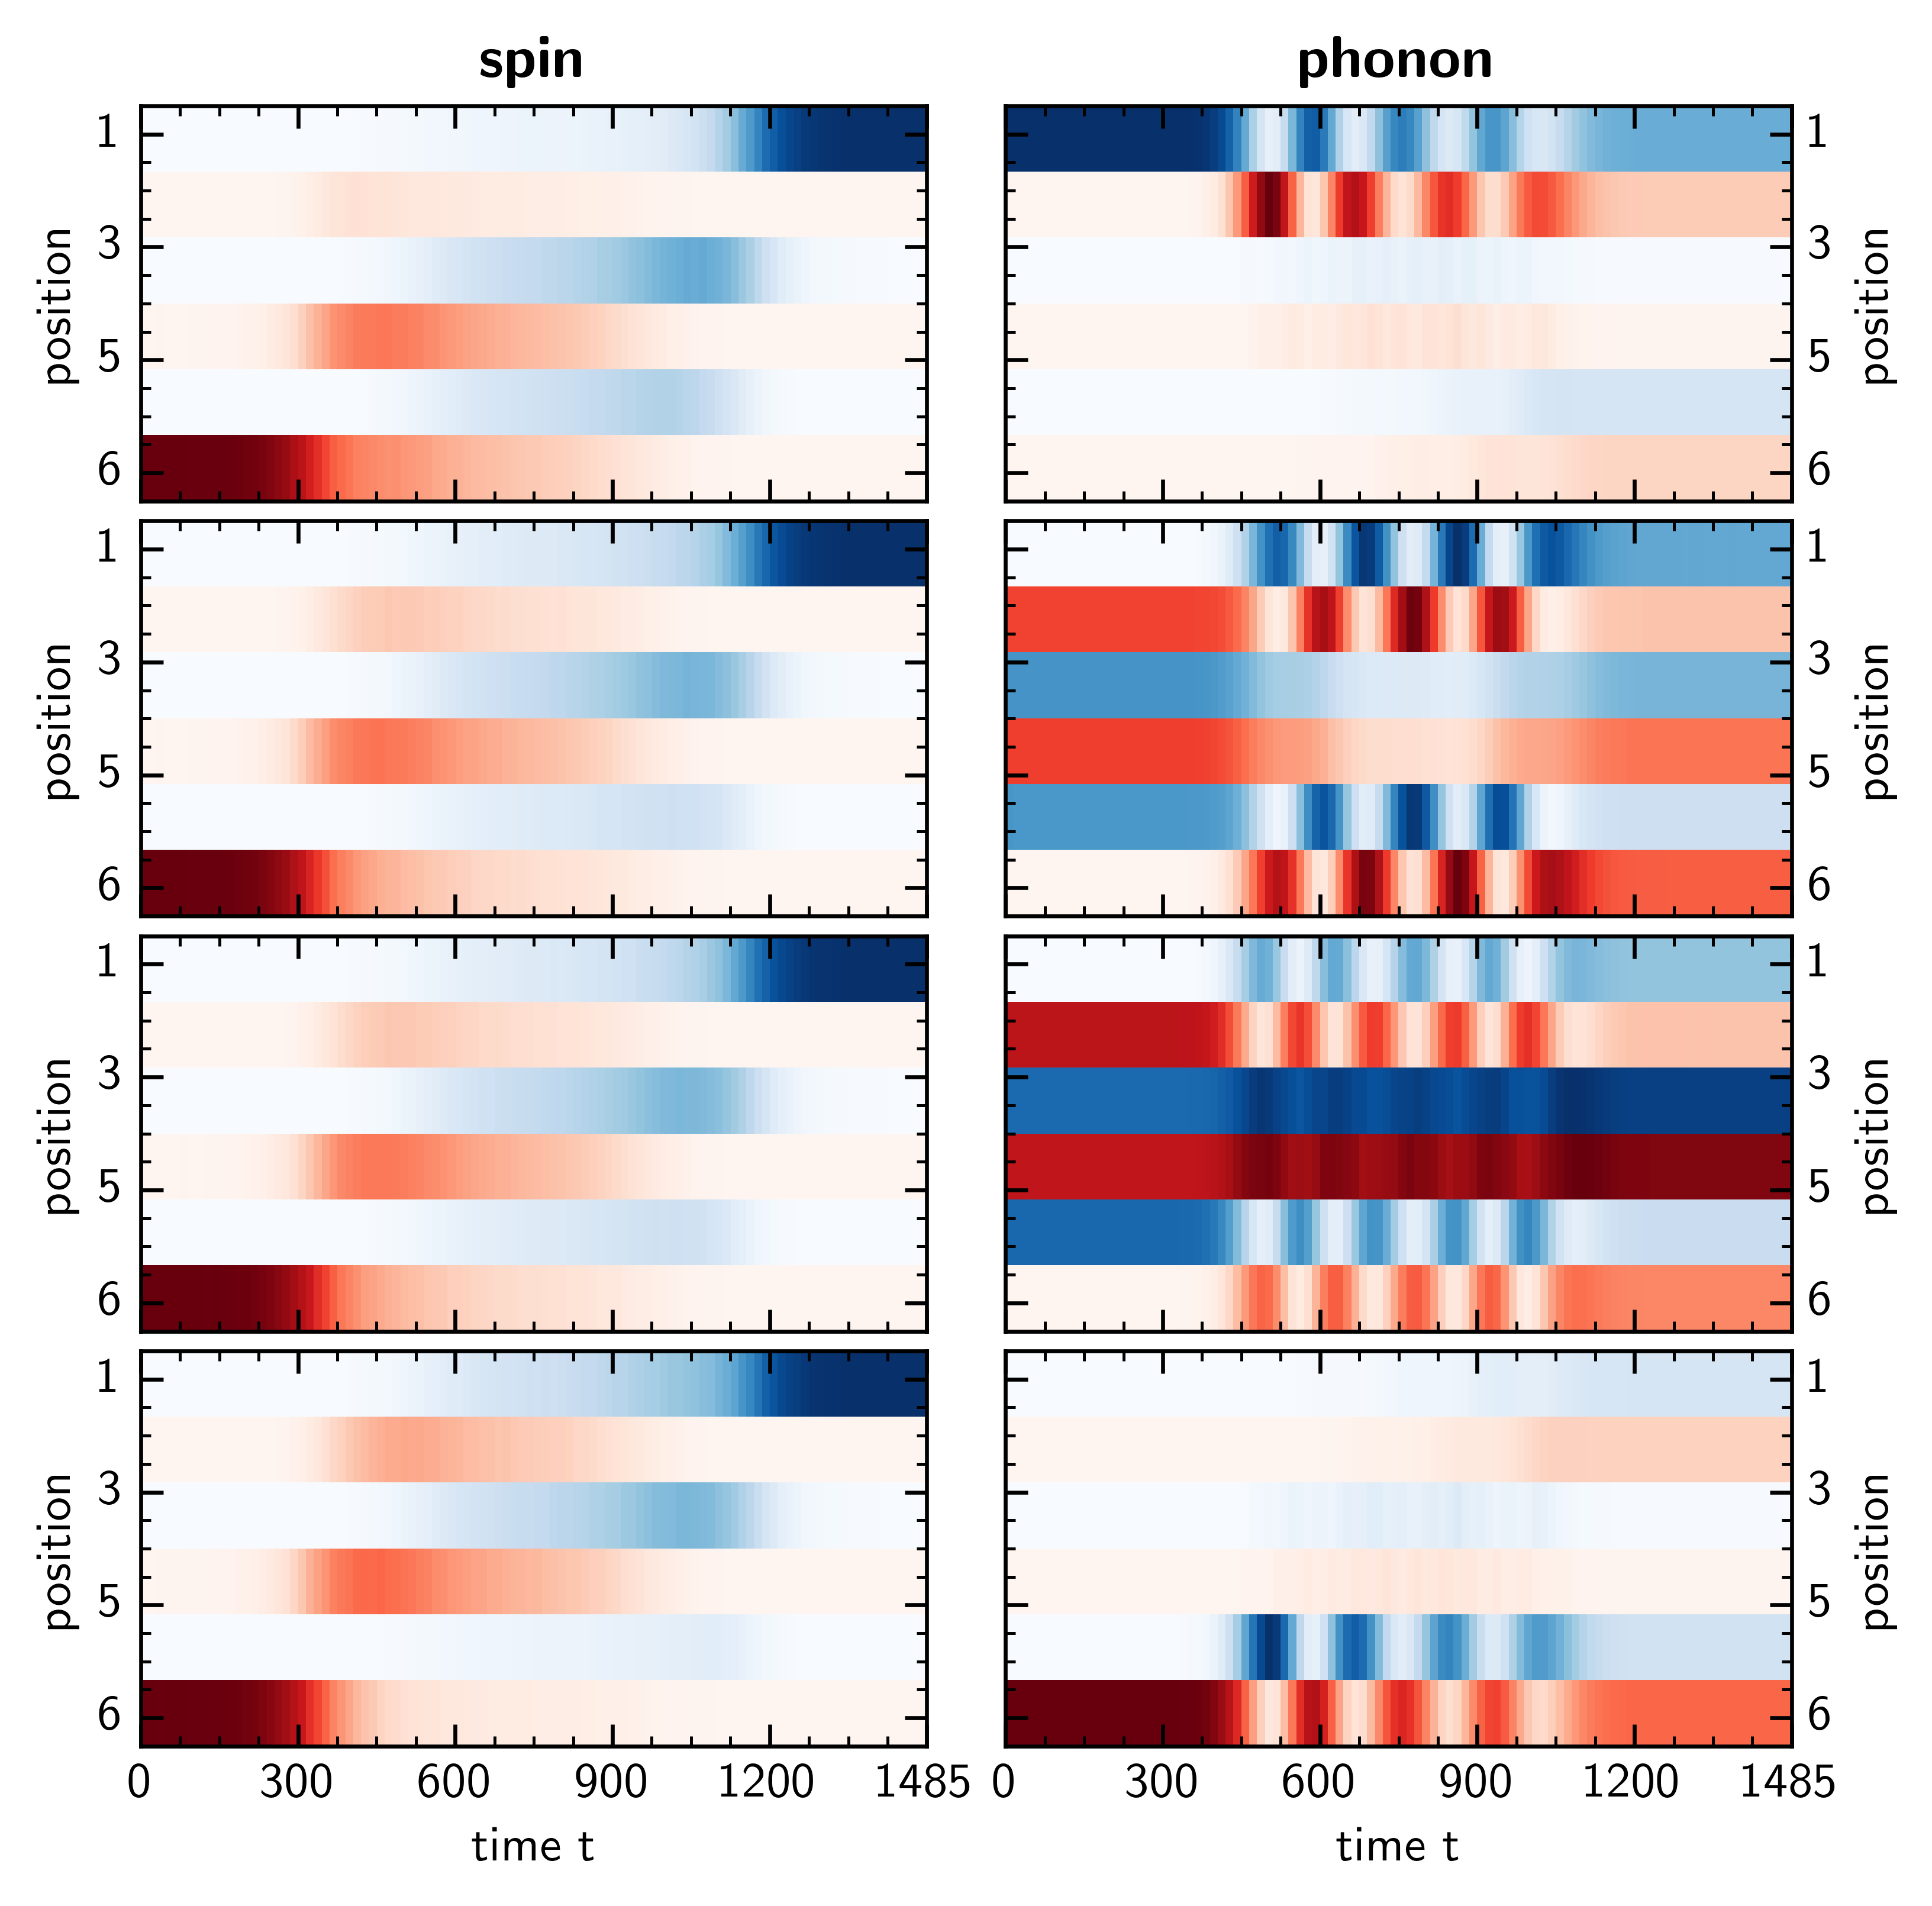
\includegraphics{pictures/spin_phonon_traj_colormap_phintc_rescale100.png}
    \caption{\textbf{Spin transfer process.} The time evolution of the spin and phonon degrees of freedom is depicted during the adiabatic transfer protocol. For the same transfer protocol the system was prepared in different initial phonon configurations, which stored one excitation in total.}
    \label{fig:transfer_trajectories}
\end{figure}

\begin{figure}[H]
    \centering
    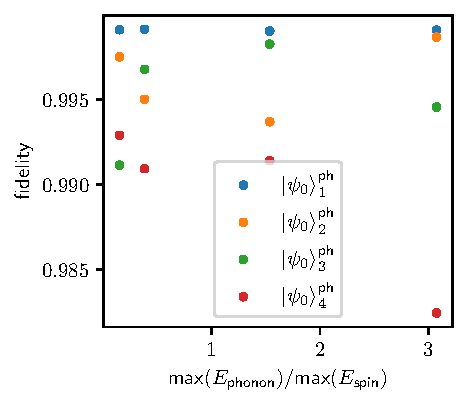
\includegraphics{pictures/fidelity_coupling_strengths.pdf}
    \caption{\textbf{Fidelity in dependence of phonon interaction strength.} For the 4 initial phonon configurations introduced in \figref{fig:transfer_trajectories} (the labeling runs from top to bottom) different rations of spin dipole interactions to phonon interactions are chosen. The fidelity between the final and target state is shown in dependence of interaction ratio and initial phonon state.}
    \label{fig:fidelity}
\end{figure}

\begin{figure}[H]
    \centering
    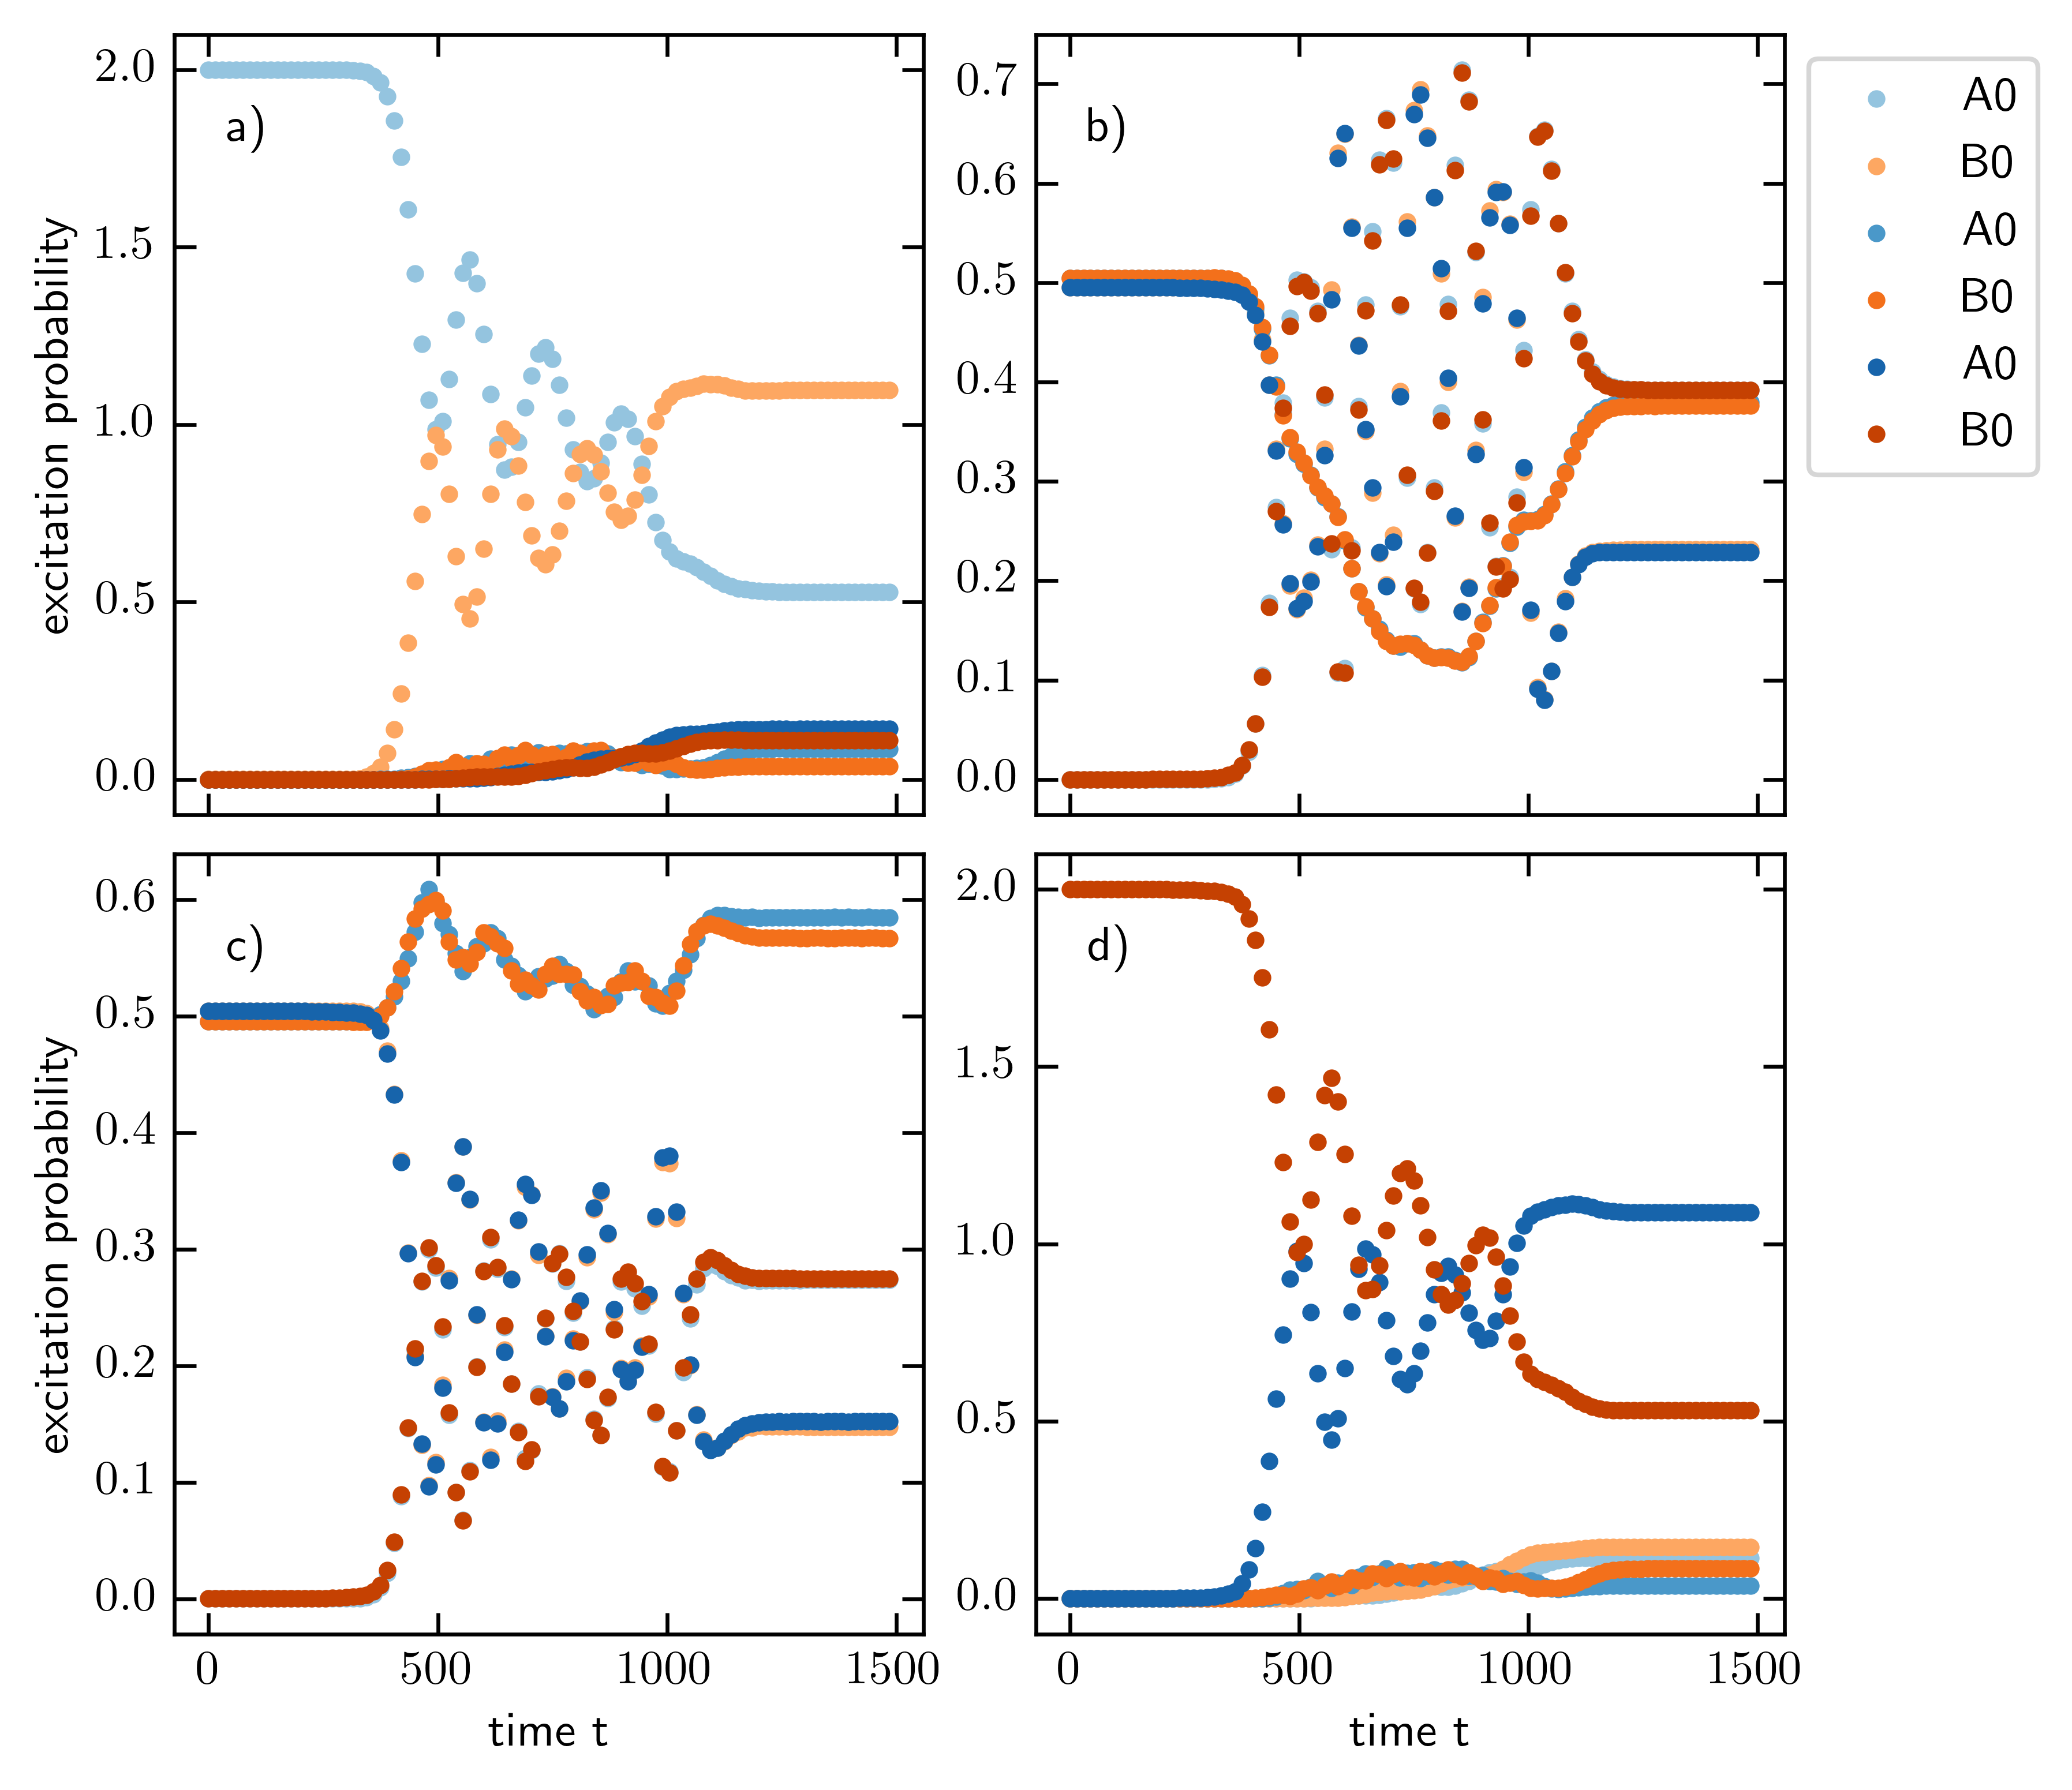
\includegraphics{pictures/spin_phonon_traj_lines_phintc_rescale100_2ph.png}
    \caption{\textbf{Phonon evolution for two excitations.} For two phonon excitations the evolution of the phonons during the transfer period is depicted.}
    \label{fig:2phonon_exc_traj}
\end{figure}


\section*{Winding number of the spin-phonon coupled Hamiltonian}
Next I want to determine the topological phase of the Hamiltonian where spin and and motional degrees of freedom are coupled in first order Schrieffer-Wolff approximation. I will again consider only nearest neighbor interaction and will also constrain the dynamics to the single excitation subspace, both in spin and phonon degrees of freedom. For this purpose I will write the interactions in terms of fermionic spin and phonon operators. $a_i$ and $b_i$ ($p_{A,i}$ and $p_{B,i}$) are spin (phonon) annihilation operators acting, respectively, on the sublattice $A$ and $B$ sites in unit cell $i$. The Hamiltonian then reads 
\begin{align*}
    H &= H_\text{sp}+H_\text{spph}\\
    \text{with}\quad H_\text{sp} &= \sum_i V_1\,a_i^\dagger b_i + V_2\,b_i^\dagger a_{i+1} +\text{h.c.}\\
    H_\text{spph}&= \sum_i V_3\,\left[ p_{A,i}^\dagger p_{B,i} + p_{B,i}^\dagger p_{A,i} - p_{A,i}^\dagger p_{A,i} - p_{B,i}^\dagger p_{B,i} \right]\,a_i^\dagger b_i +\text{h.c.}\\
    &+\sum_i V_4\,\left[ p_{A,i+1}^\dagger p_{B,i} + p_{B,i}^\dagger p_{A,i+1} - p_{A,i+1}^\dagger p_{A,i+1} - p_{B,i}^\dagger p_{B,i} \right]\,a_{i+1}^\dagger b_i +\text{h.c.}
\end{align*}
Here the intracell couplings $V_1$, $V_3$, and the intercell couplings $V_2$, $V_4$ are constants which depend on the parameters distance and dipole moment. Transforming this Hamiltonian into momentum space by simply performing a Fourier transform of every operator does not simplify the description and does not allow for an analysis of the winding number.

But by building collective operators of spin and phonon degrees of freedom one is able to make use of the one dimensional character of the chain and achieve a momentum space Hamiltonian with decoupled momenta. First I restrict myself to the spin phonon coupled term of the Hamiltonian. I group all operators in $H_\text{spph}$ acting on the same sublattice together and combine them into one operator, defined on an adapted space. By this procedure I get a couple of new operators. All of them act on the same space, which is defined on one site.
\begin{align*}
    \begin{pmatrix}
        s_i^\uparrow p_i^\uparrow\\
        s_i^\uparrow p_i^\downarrow\\
        s_i^\downarrow p_i^\uparrow\\
        s_i^\downarrow p_i^\downarrow
    \end{pmatrix}=\vcentcolon \begin{pmatrix}
        \ket{1}\\
        \ket{2}\\
        \ket{3}\\
        \ket{4}
    \end{pmatrix}
\end{align*}

For $D\in\{A,B\}$ and $d\in\{a,b\}$ I define
\begin{align*}
    c^{\bar{D},D}_i\vcentcolon&=p_{D,i}^\dagger d_i = \ket{3}\bra{2}\\
    c^{D,\bar{D}}_i\vcentcolon&=p_{D,i}\,d_i^\dagger = \ket{2}\bra{3}\\
    c^{\bar{D},\bar{D}}_i\vcentcolon&=p_{D,i}^\dagger d_i^\dagger = \ket{1}\bra{4}\\
    c^{D,D}_i\vcentcolon&=p_{D,i}\, d_i = \ket{4}\bra{1}\\
    c^{\bar{D}}_i\vcentcolon&= d_i^\dagger = \ket{1}\bra{3}+\ket{2}\bra{4}\\
    c^{D}_i\vcentcolon&= d_i = \ket{3}\bra{1}+\ket{4}\bra{2}\\
    c^{\bar{D},D,D}_i\vcentcolon&=p_{D,i}^\dagger p_{D,i}\, d_i = \ket{3}\bra{1}\\
    c^{\bar{D},D,\bar{D}}_i\vcentcolon&=p_{D,i}^\dagger p_{D,i}\, d_i^\dagger = \ket{1}\bra{3}\,
\end{align*}
what lets the Hamiltonian read
\begin{align*}
    H_\text{spph}&= \sum_i V_3\,\left[ c_i^{\bar{A},\bar{A}}\,c_i^{B,B} + c_i^{A,\bar{A}}\,c_i^{\bar{B},B} - c_i^{\bar{A},A,\bar{A}}\,c_i^{B} - c_i^{\bar{A}}\,c_i^{\bar{B},B,B}\right] +\text{h.c.}\\
    &+ \sum_i V_4\,\left[ c_{i+1}^{\bar{A},\bar{A}}\,c_i^{B,B} + c_{i+1}^{A,\bar{A}}\,c_i^{\bar{B},B} - c_{i+1}^{\bar{A},A,\bar{A}}\,c_i^{B} - c_{i+1}^{\bar{A}}\,c_i^{\bar{B},B,B}\right] +\text{h.c.}
\end{align*}
Because of the single excitation restriction, exactly one phonon and spin has to be present at the two neighboring sites for a term acting on those two neighboring sites to contribute. Therefore the combined space of the two neighboring sites collapses to the dimensin of the one site space, represented by the basis
\begin{align*}
    \begin{pmatrix}
        s_1^\uparrow p_1^\uparrow \; s_2^\downarrow p_2^\downarrow\\
        s_1^\uparrow p_1^\downarrow\; s_2^\downarrow p_2^\uparrow\\
        s_1^\downarrow p_1^\uparrow\; s_2^\uparrow p_2^\downarrow\\
        s_1^\downarrow p_1^\downarrow\; s_2^\uparrow p_2^\uparrow
    \end{pmatrix}
\end{align*}
The Hamiltonian in $k$-space then reads
\begin{align*}
    H_\text{spph}&= \sum_k V_3\,\left[ c_k^{\bar{A},\bar{A}}\,c_k^{B,B} + c_k^{A,\bar{A}}\,c_k^{\bar{B},B} - c_k^{\bar{A},A,\bar{A}}\,c_k^{B} - c_k^{\bar{A}}\,c_k^{\bar{B},B,B}\right] +\text{h.c.}\\
    &+ \sum_k V_4\,e^{ika}\,\left[ c_k^{\bar{A},\bar{A}}\,c_k^{B,B} + c_k^{A,\bar{A}}\,c_k^{\bar{B},B} - c_k^{\bar{A},A,\bar{A}}\,c_k^{B} - c_k^{\bar{A}}\,c_k^{\bar{B},B,B}\right] +\text{h.c.}\\
    &= \sum_k \left(V_3+V_4\,e^{ika}\right)\,\left[ c_k^{\bar{A},\bar{A}}\,c_k^{B,B} + c_k^{A,\bar{A}}\,c_k^{\bar{B},B} - c_k^{\bar{A},A,\bar{A}}\,c_k^{B} - c_k^{\bar{A}}\,c_k^{\bar{B},B,B}\right] +\text{h.c.}\\
    &=\vcentcolon \sum_k H_\text{spph}^k
\end{align*}
The blocks in $k$-space then read
\begin{align*}
    H_\text{spph}= \begin{pmatrix}
        0 & 0 & -(V_3+V_4\,e^{ika}) & V_3+V_4\,e^{ika}\\
        0 & 0 & V_3+V_4\,e^{ika} & -(V_3+V_4\,e^{ika})\\
        -(V_3+V_4\,e^{-ika}) & V_3+V_4\,e^{-ika} & 0 & 0 \\
       V_3+V_4\,e^{-ika} & -(V_3+V_4\,e^{-ika}) & 0 & 0         
    \end{pmatrix}
\end{align*}
When considering the total Hamiltonian including $H_\text{sp}$ one has to expand the space for the collective operators as now the Hamiltonian does not only couple states where spin and phonon excitations are next to each other. But only two new states have to be introduced, $s_1^\uparrow p_1^\downarrow \; s_2^\downarrow p_2^\downarrow$ and $s_1^\downarrow p_1^\downarrow\; s_2^\uparrow p_2^\downarrow$. The basis is now family
\begin{align*}
    \begin{pmatrix}
        s_1^\uparrow p_1^\uparrow \; s_2^\downarrow p_2^\downarrow\\
        s_1^\uparrow p_1^\downarrow\; s_2^\downarrow p_2^\uparrow\\
        s_1^\uparrow p_1^\downarrow \; s_2^\downarrow p_2^\downarrow\\
        s_1^\downarrow p_1^\uparrow\; s_2^\uparrow p_2^\downarrow\\
        s_1^\downarrow p_1^\downarrow\; s_2^\uparrow p_2^\uparrow\\
        s_1^\downarrow p_1^\downarrow\; s_2^\uparrow p_2^\downarrow
    \end{pmatrix}=\vcentcolon \begin{pmatrix}
        \ket{1}\\
        \ket{2}\\
        \ket{3}\\
        \ket{4}\\
        \ket{5}\\
        \ket{6}
    \end{pmatrix}
\end{align*}
In this basis the spin Hamiltonian in momentum space $H_\text{sp}^k$ reads
\begin{align*}
    H_\text{sp}^k &= \begin{pmatrix}
        0&\alpha\\
        \alpha^\dagger&0
    \end{pmatrix}\\
    \text{with}\quad\alpha&= \left(V_1+V_2\,e^{ika}\right)\,\begin{pmatrix}
        1&0&0\\
        0&1&0\\
        0&0&1
    \end{pmatrix}
\end{align*}
The total Hamiltonian in momentum space thus reads
\begin{align*}
    H^k &= \begin{pmatrix}
        0&\beta\\
        \beta^\dagger&0
    \end{pmatrix}\\
    \text{with}\quad\beta&=\begin{pmatrix}
        V_1-V_3+(V_2-V_4)\,e^{ika}&V_3+V_4\,e^{ika}&0\\
        V_3+V_4\,e^{ika}&V_1-V_3+(V_2-V_4)\,e^{ika}&0\\
        0&0&V_1+V_2\,e^{ika}
    \end{pmatrix}
\end{align*}
The eigenvalues of $\beta$ are
\begin{align*}
    \beta_1 &= V_1-2\,V_3+(V_2-2\,V_4)\,e^{ika}\\
    \beta_2 = \beta_3 &= V_1+V_2\,e^{ika}
\end{align*}
\subsection*{Problems}
The main practical problem is that the total Hamiltonian is heavily degenerate $\sim N$. The winding number can however only take values between $0$ and $3$. Which eigenvalues are the topological protected ones?

This might be not due to an erroneous derivation of the momentum space Hamiltonian. But I don't know. At first glance there is a problem with the kernel of the Hamiltonian. In real space it has a finite dimension of the magnitude of $N$. But in momentum space the kernel seems to vanish. I think the reason is that I only considered a basis for the combined coupling operators, which actually couple, hence discarding the kernel. But I think this is no unusual proceed. I don't know if the winding number is valid for degenerate Hamiltonians. 

\begin{itemize}
\item Go to higher dimensions, e.g. transport on the closed surface of a 2D-lattice
\item Spin-phonon coupling:%\\
% $H = H_\text{sp}+ H_\text{sp-ph}$
\begin{itemize}
\item What effect has the spin-phonon coupling on transport performance?
\item Is it possible to transport both spins and phonons simultaneously?
\end{itemize}
\end{itemize}
\newpage
\subsection*{Spin-phonon coupling} 
$$H=\sum_j H_\text{ph}^{j,j+1} a_j^\dagger a_{j+1} + \text{h.c.}$$
with 
$$H_\text{ph}^{j,j+1}=V_{j,j+1}^\text{der}\left(p_j^\dagger p_{j+1}+p_{j+1}^\dagger p_{j}-p_{j}^\dagger p_{j}-p_{j+1}^\dagger p_{j+1}\right)$$
$a_j$ and $p_j$ are spin and phonon annihilation operators respectively.
\subsubsection*{Attempt of analytic solution for the time evolution (3 atoms)}
I'm considering 3 atoms with the Hamiltonian 
\begin{align*}
H&=H_{12}a^\dagger b+H_{23}b^\dagger c +\text{h.c.}\\
\text{with}\quad H_{ij}&=p_i^\dagger p_{j}+p_{j}^\dagger p_{i}-p_{i}^\dagger p_{i}-p_{j}^\dagger p_{j}
\end{align*}
I want to calculate the time evolution of the occupation operator $a^\dagger a$.
$$a^\dagger a(t) = e^{iHt}a^\dagger a e^{-iHt}=\sum_n\frac{(it)^n}{n!} [H,a^\dagger a]_n=:\sum_n\frac{(it)^n}{n!}\,C_n$$
with $[H,a^\dagger a]_n = [H,[H,a^\dagger a]_{n-1}]$.
$$C_2 = 2 H_{12}^2 (a^\dagger a - b^\dagger b) + H_{23} H_{12} c^\dagger a + H_{12} H_{23} a^\dagger c $$ $$C_3 = (4 H_{12}^3 + H_{23}^2 H_{12}) b^\dagger a - (4 H_{12}^3 + H_{12} H_{23}^2) a^\dagger b - 3 H_{23} H_{12}^2 c^\dagger b + 3 H_{12}^2 H_{23} b^\dagger c $$

$$ C_4 = (8 H_{12}^4 + 2 H_{12} H_{23}^2 H_{12}) a^\dagger a - \left(8 H_{12}^4 + 4 H_{12}^2 H_{23}^2 + 4 H_{23}^2 H_{12}^2 \right) b^\dagger b + 6 H_{23} H_{12}^2 H_{23} c^\dagger c  $$$$+ (7 H_{23} H_{12}^3 + H_{23}^3 H_{12}) c^\dagger a + (7 H_{12}^3 H_{23} + H_{12} H_{23}^3) a^\dagger c$$
Concentrating on the odd indices one can determine a recursion relation for the coefficients of $a^\dagger b$ and $b^\dagger c$. 
\begin{align*}
    c_{ab}'&=H_{12}^2\,c_{ab}+c_{ab}\,(H_{12}^2+H_{23}^2)+2H_{12}\,c_{ab}^\dagger \,H_{12}-2H_{12}\,c_{bc}\,H_{23}-H_{12}H_{23}\,c_{bc}^\dagger  \\\\
    c_{bc}'&=(H_{12}^2+H_{23}^2)\,c_{bc}+c_{bc}\,H_{23}^2+2H_{23}\,c_{bc}^\dagger \,H_{23}-2H_{12}\,c_{ab}\,H_{23}-c_{ab}^\dagger\, H_{12}H_{23} 
\end{align*}
By redefining the coefficients as
$$c_{ab}=\vcentcolon H_{12}\,\alpha  ,\quad c_{bc}=\vcentcolon \beta\,H_{23}$$
one can reach at a slightly simpler recursion relation
$$\alpha_{n+1}=H_{12}^2\,\alpha_n +\alpha_n \,(H_{12}^2+H_{23}^2)+2\alpha_n ^\dagger \,H_{12}^2+2\beta_n\,H_{23}^2+H_{23}^2\,\beta_n^\dagger$$
$$\beta_{n+1} = (H_{12}^2+H_{23}^2)\,\beta_n + \beta_n\, H_{23}^2 + 2H_{23}^2\,\beta_n^\dagger + 2H_{12}^2\,\alpha_n + \alpha_n^\dagger\, H_{12}^2$$

\begin{figure}[H]
    \hspace*{-2.5cm}
    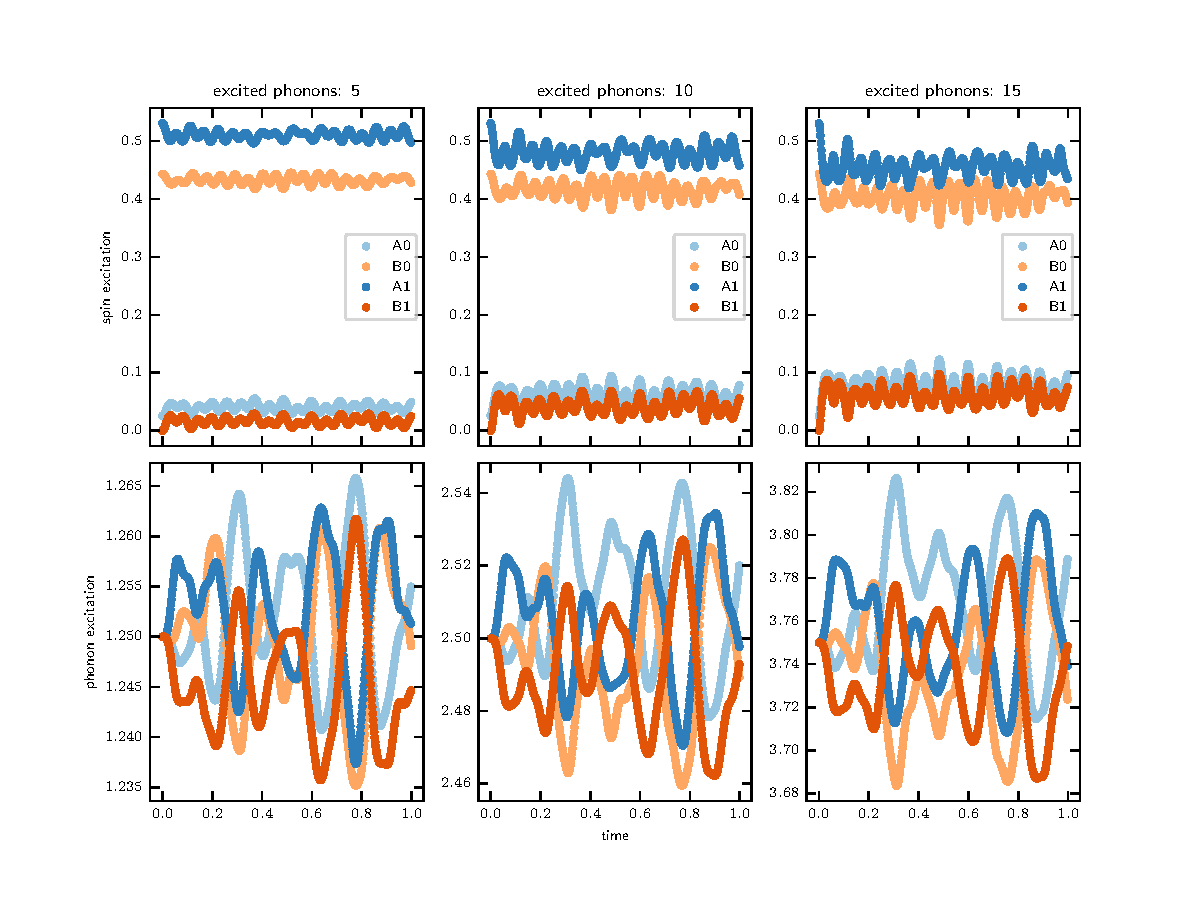
\includegraphics{pictures/chain4_only_coupling.pdf}
    \caption{\textbf{Evolution with only spin-phonon coupling term.}}
    % \label{fig:fidelity}
\end{figure}
\begin{figure}[H]
    \hspace*{-2.5cm}
    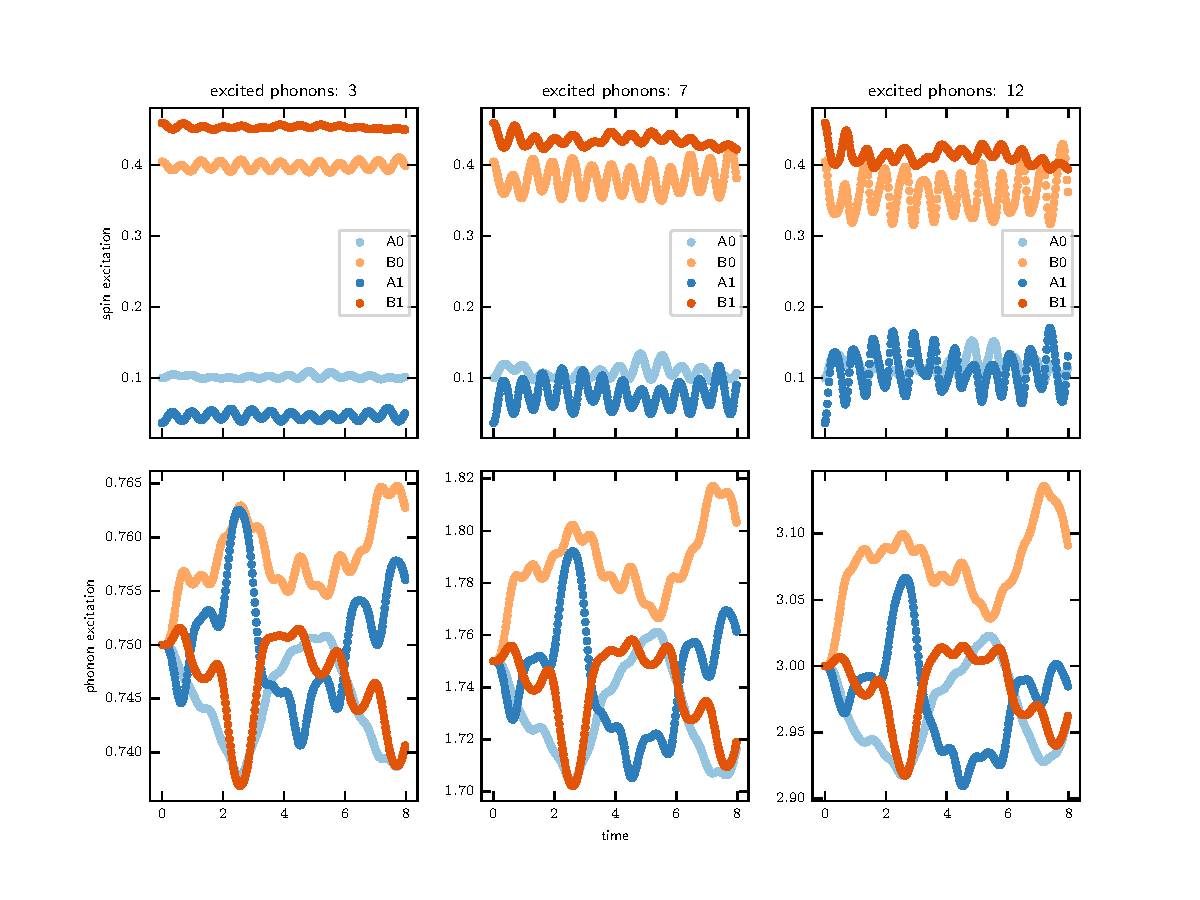
\includegraphics{pictures/chain4_spin_phonon_only.pdf}
    \caption{\textbf{Evolution with only spin-phonon coupling term.}}
    % \label{fig:fidelity}
\end{figure}
\begin{figure}[H]
    \hspace*{-2.5cm}
    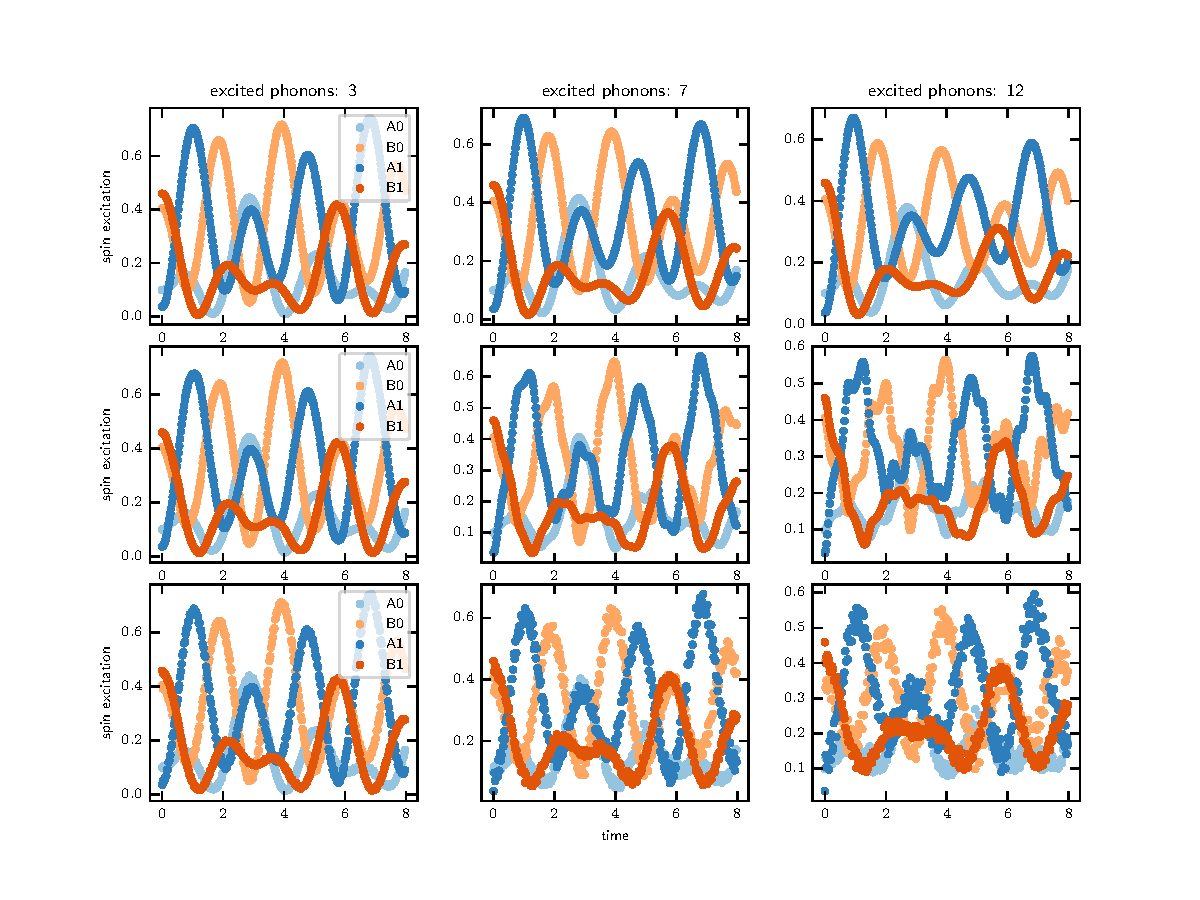
\includegraphics{pictures/chain4_free_evol_all_coupling.pdf}
    \caption{\textbf{Summary spin evolution}}
    % \label{fig:fidelity}
\end{figure}
\begin{figure}[H]
    \hspace*{-2.5cm}
    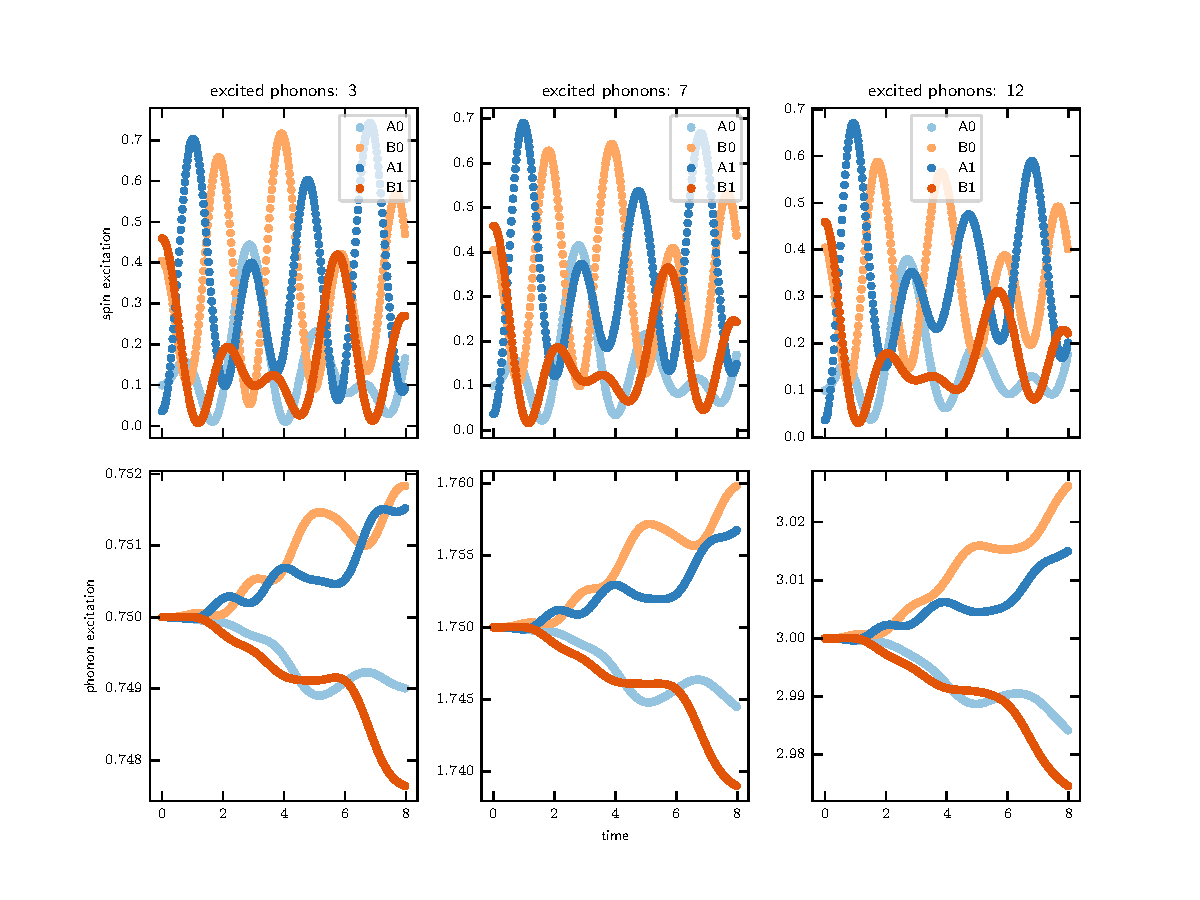
\includegraphics{pictures/chain4_free_evol_1spto1tenthcoupling.pdf}
    \caption{\textbf{Evolution with full Hamiltonian ratio spin only: coupling 10:1.}}
    % \label{fig:fidelity}
\end{figure}
\begin{figure}[H]
    \hspace*{-2.5cm}
    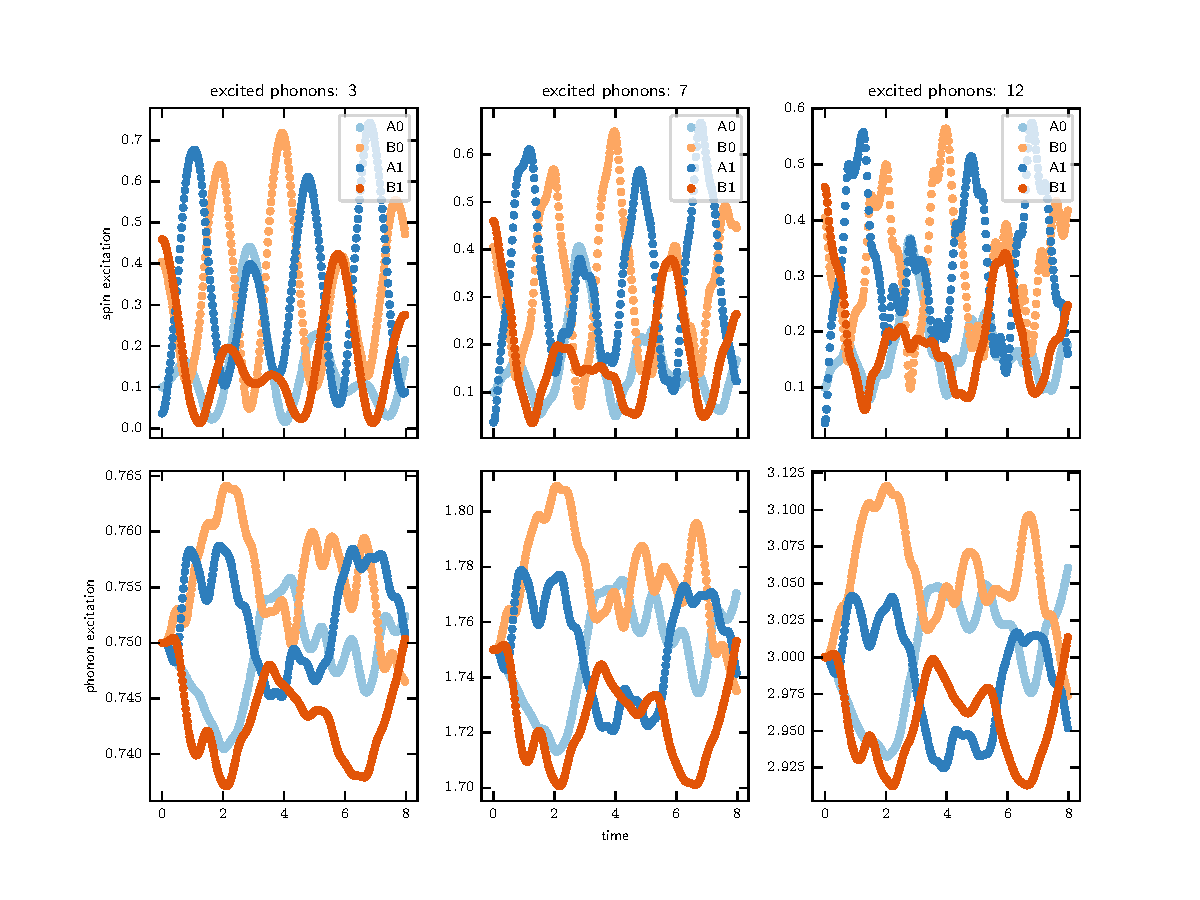
\includegraphics{pictures/chain4_free_evol_1spto1coupling.pdf}
    \caption{\textbf{Evolution with full Hamiltonian ratio spin only: coupling 1:1.}}
    % \label{fig:fidelity}
\end{figure}
\begin{figure}[H]
    \hspace*{-2.5cm}
    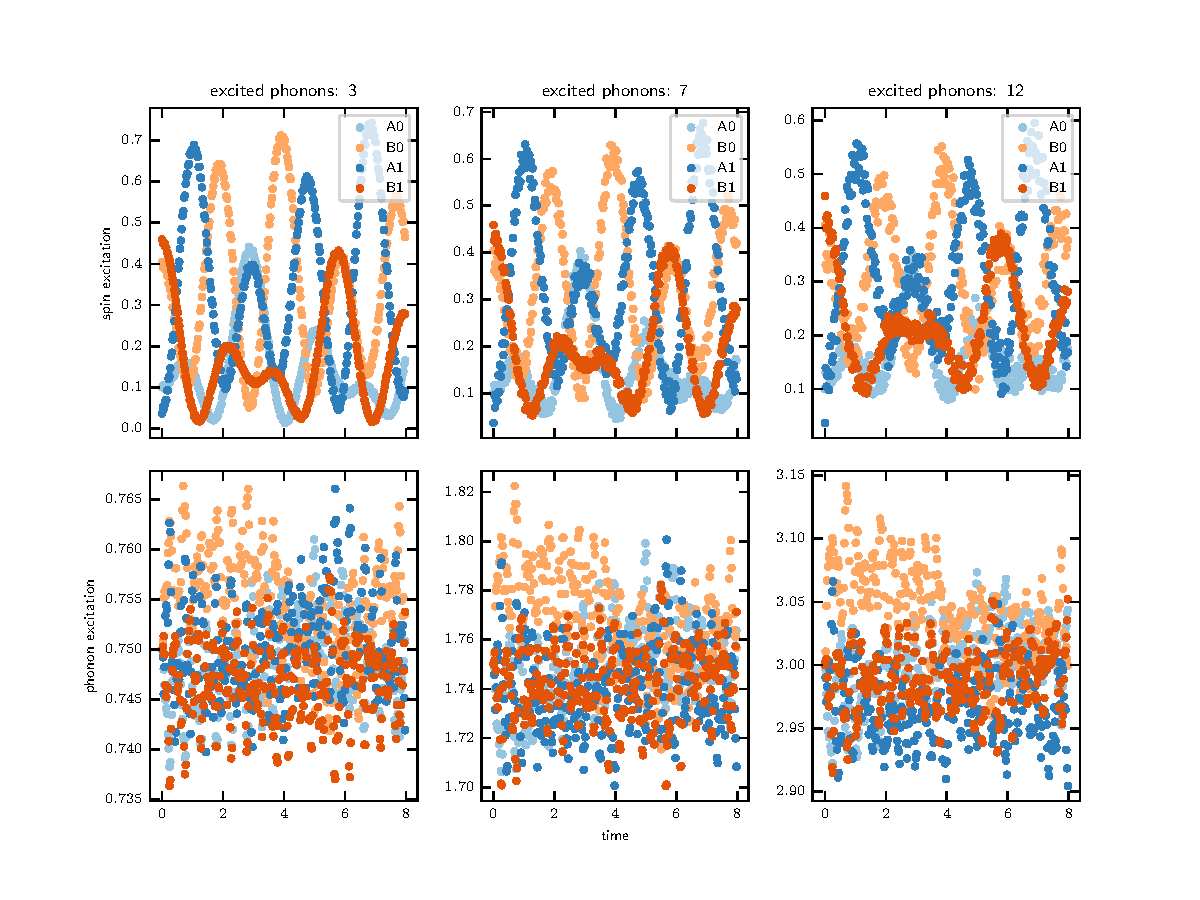
\includegraphics{pictures/chain4_free_evol_1spto10coupling.pdf}
    \caption{\textbf{Evolution with full Hamiltonian ratio spin only: coupling 1:10.}}
    % \label{fig:fidelity}
\end{figure}



\begin{figure}[H]
    \hspace*{-2.5cm}
    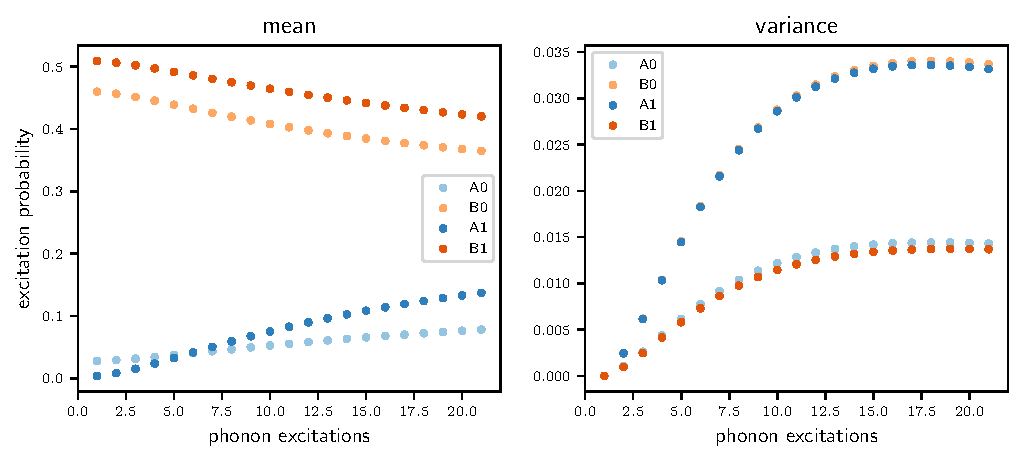
\includegraphics{pictures/chain4_spin_phonon_only_mean_variance.pdf}
    \caption{\textbf{spin-phonon coupling only.}}
    % \label{fig:fidelity}
\end{figure}
\begin{figure}[H]
    \hspace*{-2.5cm}
    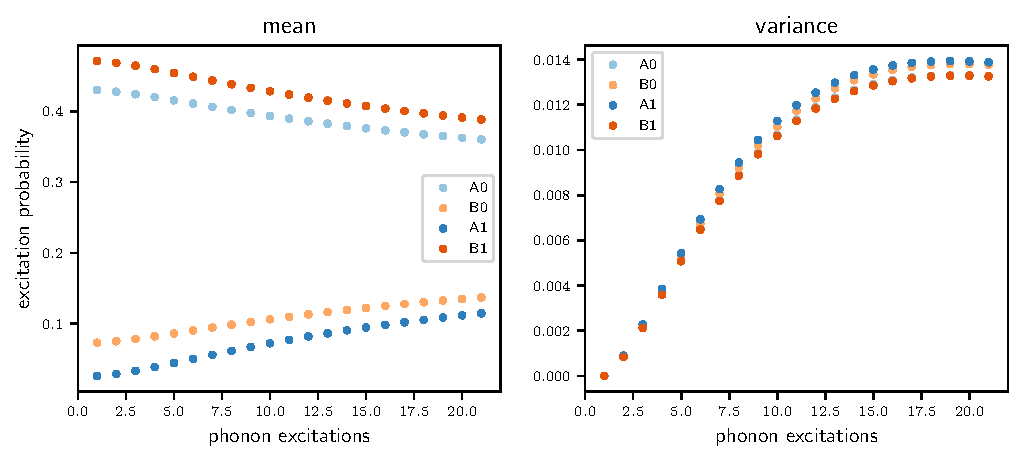
\includegraphics{pictures/chain4_spin_phonon_only_mean_variance2.pdf}
    % \caption{\textbf{spin-phonon coupling only.}}
    % \label{fig:fidelity}
\end{figure}
\begin{figure}[H]
    \hspace*{-2.5cm}
    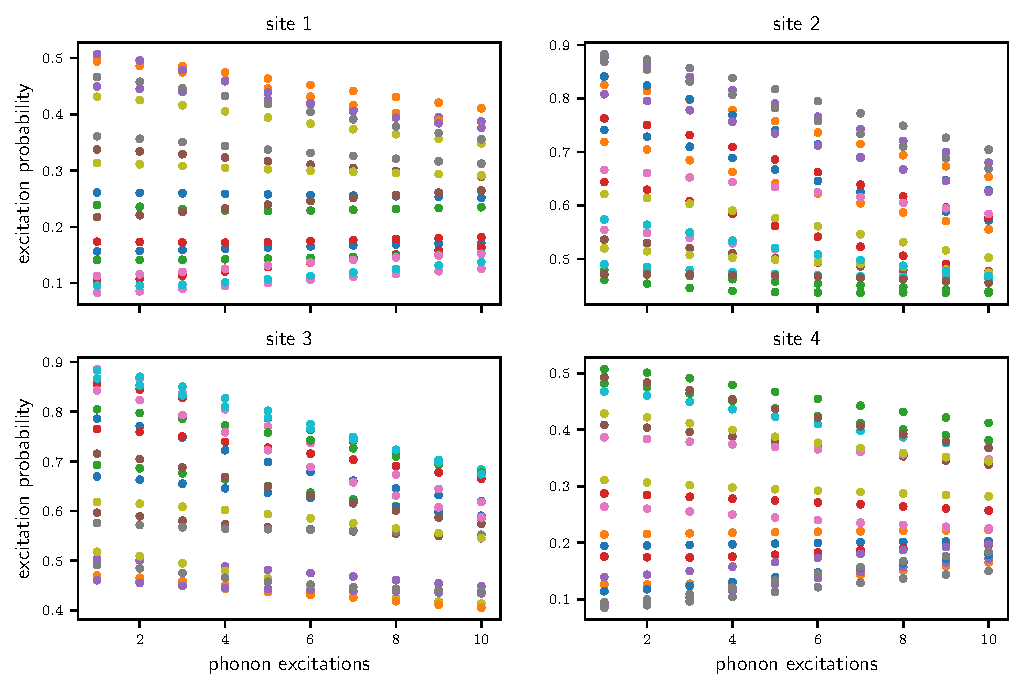
\includegraphics[scale=0.99]{pictures/chain4_maxima_dep_phnumb.pdf}
    % \caption{\textbf{spin-phonon coupling only.}}
    % \label{fig:fidelity}
\end{figure}
\begin{figure}[H]
    \hspace*{-2.5cm}
    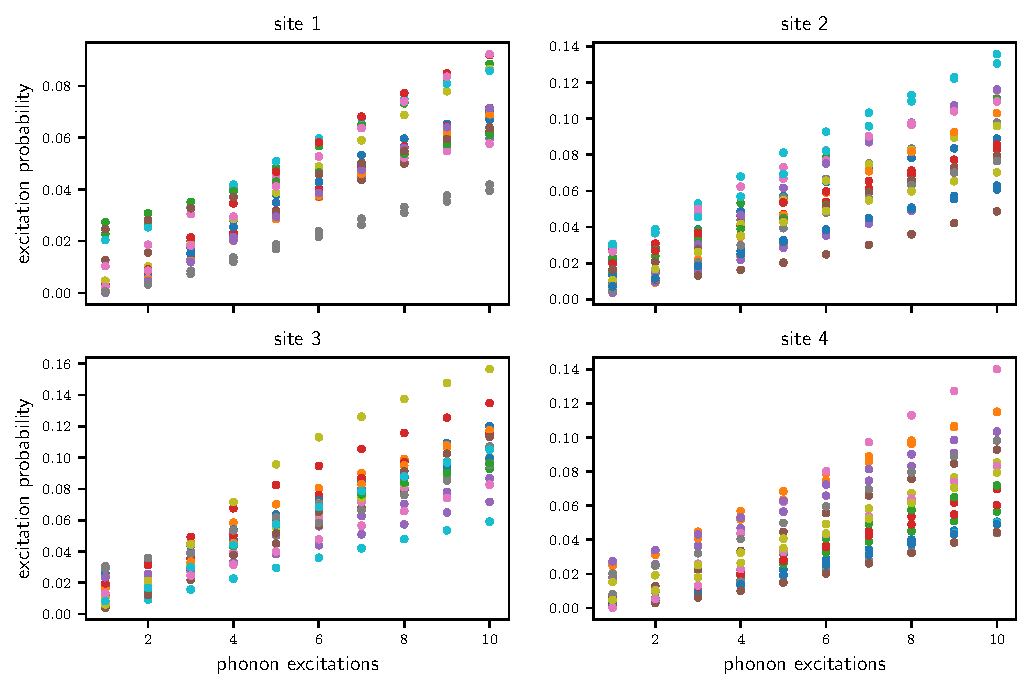
\includegraphics[scale=0.99]{pictures/chain4_minima_dep_phnumb.pdf}
    % \caption{\textbf{spin-phonon coupling only.}}
    % \label{fig:fidelity}
\end{figure}
\begin{figure}[H]
    \hspace*{-2.5cm}
    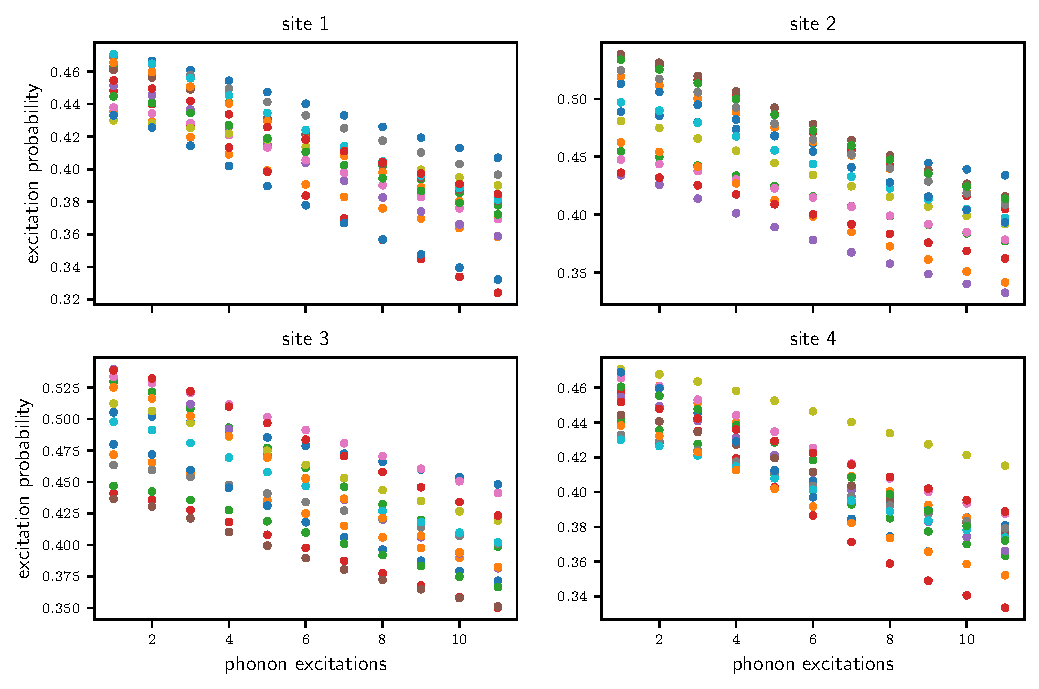
\includegraphics[scale=0.99]{pictures/chain4_maxima_dep_phnumb2.pdf}
    % \caption{\textbf{spin-phonon coupling only.}}
    % \label{fig:fidelity}
\end{figure}
\begin{figure}[H]
    \hspace*{-2.5cm}
    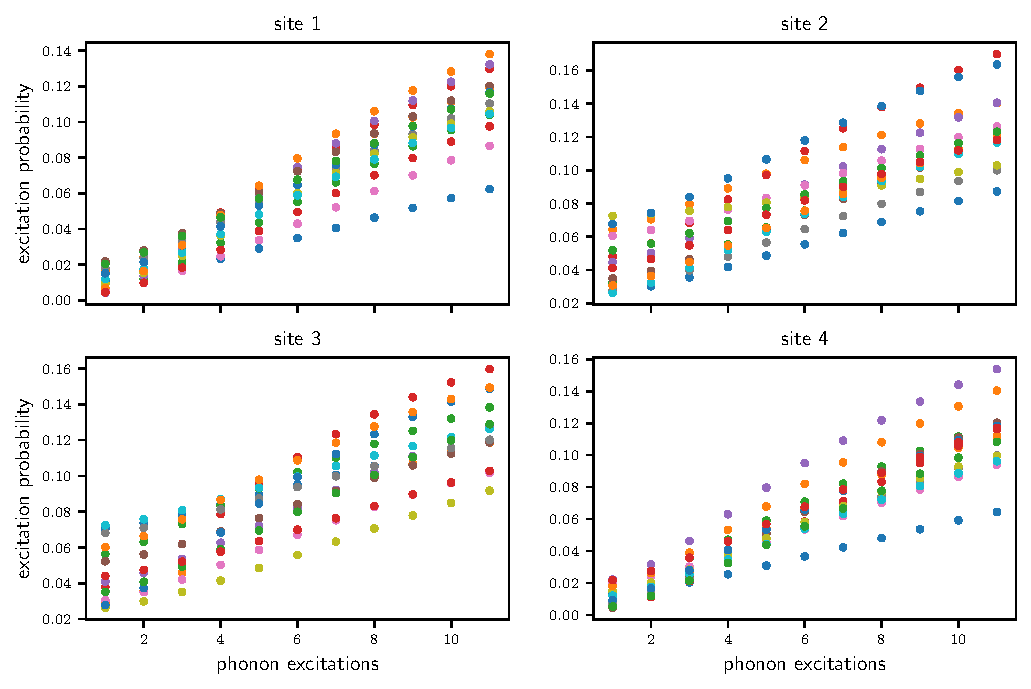
\includegraphics[scale=0.99]{pictures/chain4_minima_dep_phnumb2.pdf}
    % \caption{\textbf{spin-phonon coupling only.}}
    % \label{fig:fidelity}
\end{figure}

\begin{figure}[H]
    \hspace*{-2.5cm}
    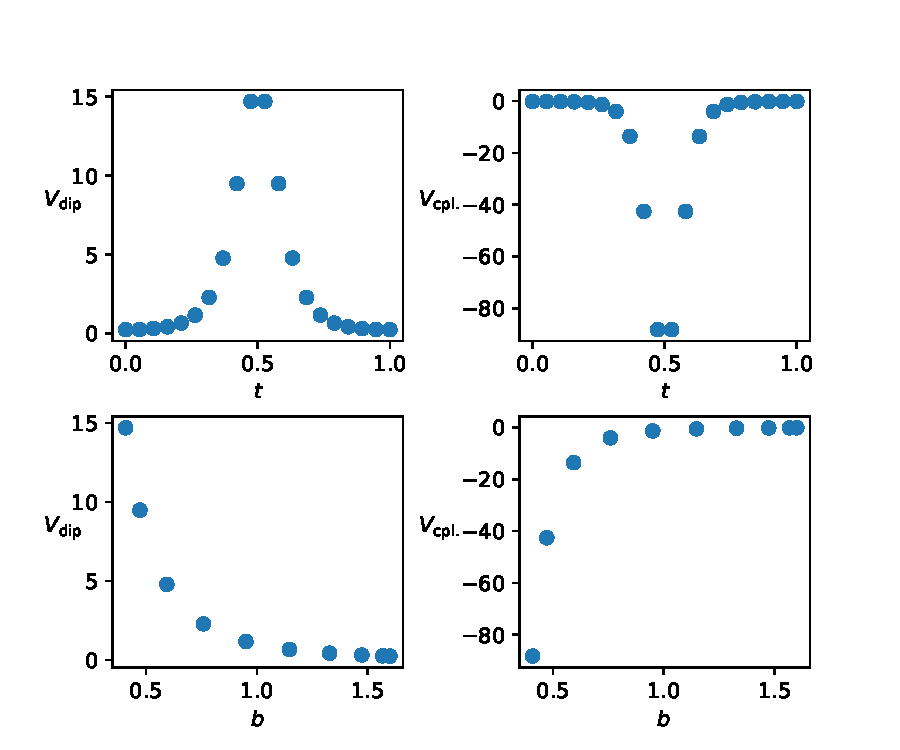
\includegraphics[scale=1]{pictures/interaction_ricemele_chain4.pdf}
    \caption{\textbf{Interaction strengths during Rice-Mele scheme.}}
    % \label{fig:fidelity}
\end{figure}
\begin{figure}[H]
    \hspace*{-2.5cm}
    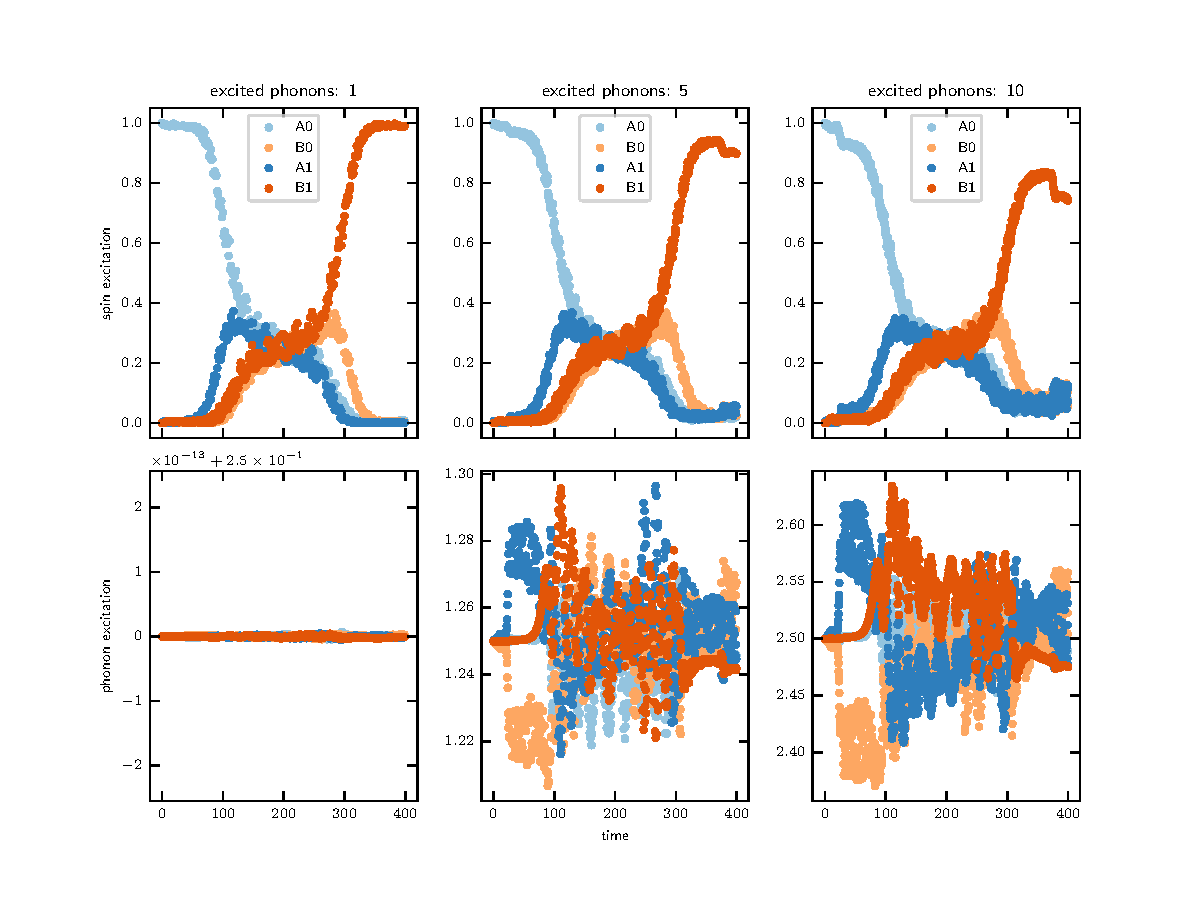
\includegraphics{pictures/chain4_ricemele_1spto10oupling.pdf}
    \caption{\textbf{Rice-Mele scheme.}}
    % \label{fig:fidelity}
\end{figure}
% \begin{figure}[H]
%     \begin{subfig}{0.5\textwidth}
%         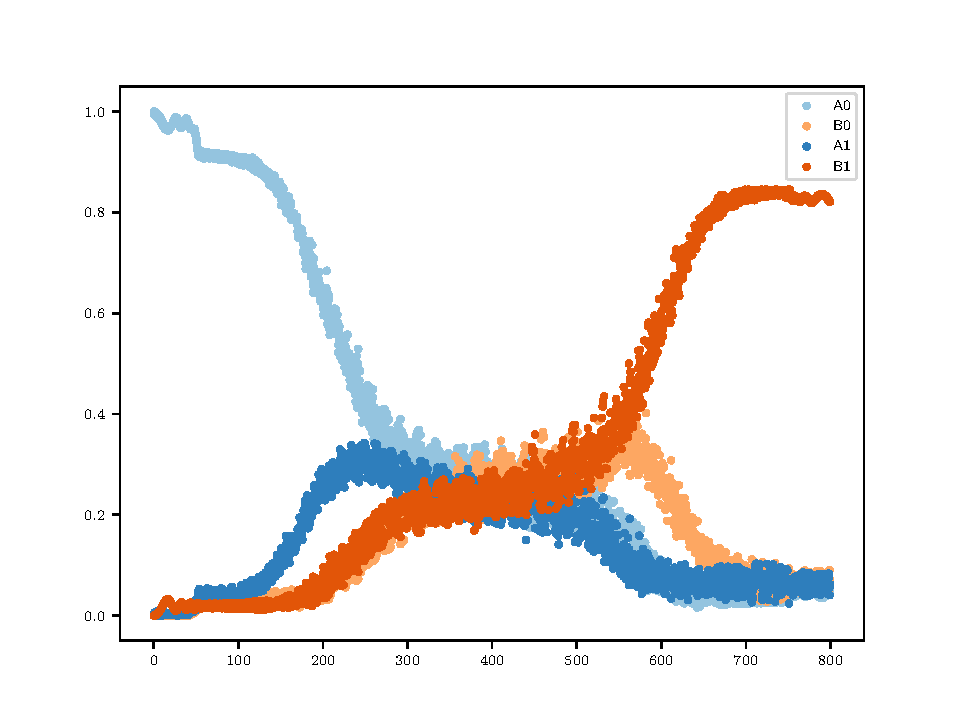
\includegraphics[scale=1]{pictures/chain4_ricemele_1spto10oupling_doubletime_10phonons.pdf.pdf}
%         \caption{\textbf{Rice-Mele scheme with longer time evolution.}}
%     \end{subfig}
%     \begin{subfig}{0.5\textwidth}
%         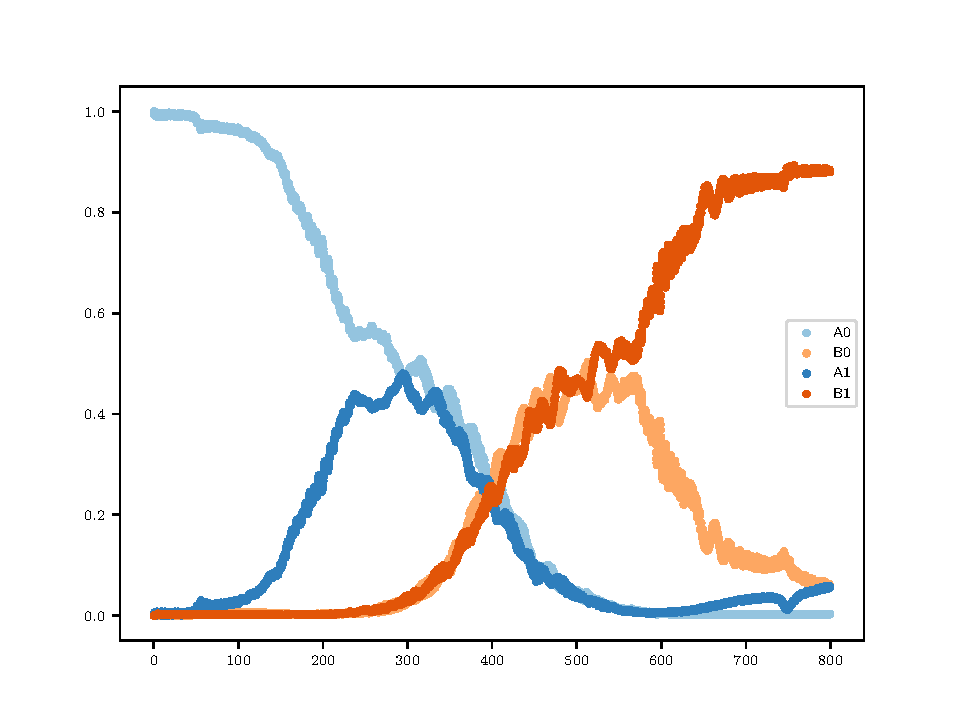
\includegraphics[scale=1]{pictures/chain4_ricemele_1spto10oupling_doubletime_10phonons_Delta10.pdf}
%         \caption{\textbf{Rice-Mele scheme with longer time evolution with $\Delta$ 10 times higher.}}
%     \end{subfig}
% \end{figure}
\begin{figure}[H]
    \centering

    % --- Left subplot ---
    \begin{subfigure}[b]{0.48\textwidth}
        \centering
        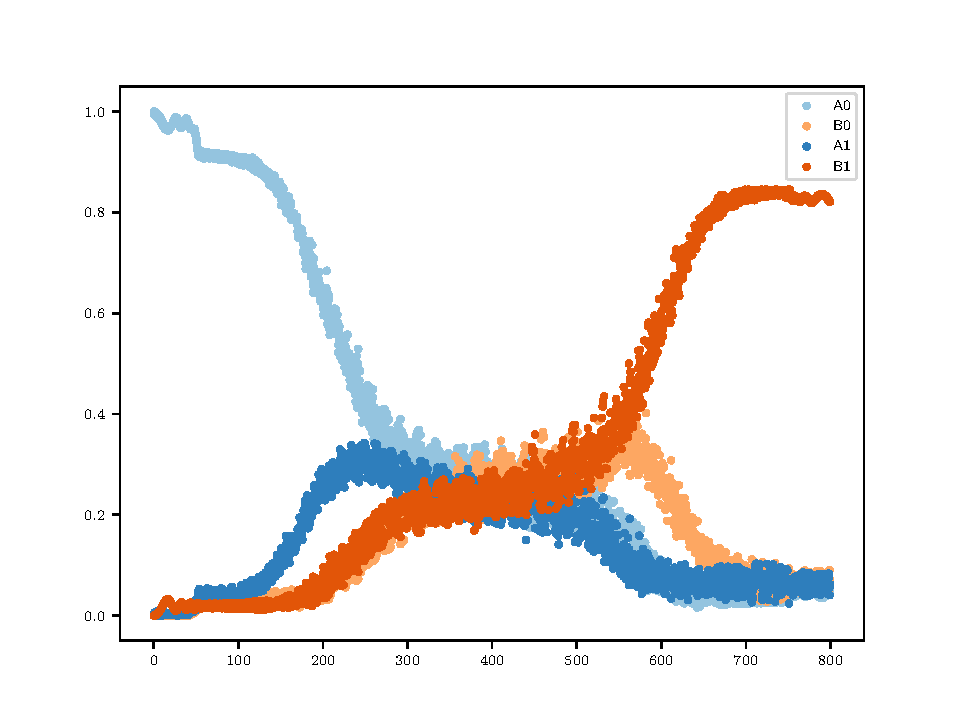
\includegraphics[width=\textwidth]{pictures/chain4_ricemele_1spto10oupling_doubletime_10phonons.pdf}
        \caption{$\Delta=1$}
        \label{fig:image1}
    \end{subfigure}
    \hfill
    % --- Right subplot ---
    \begin{subfigure}[b]{0.48\textwidth}
        \centering
        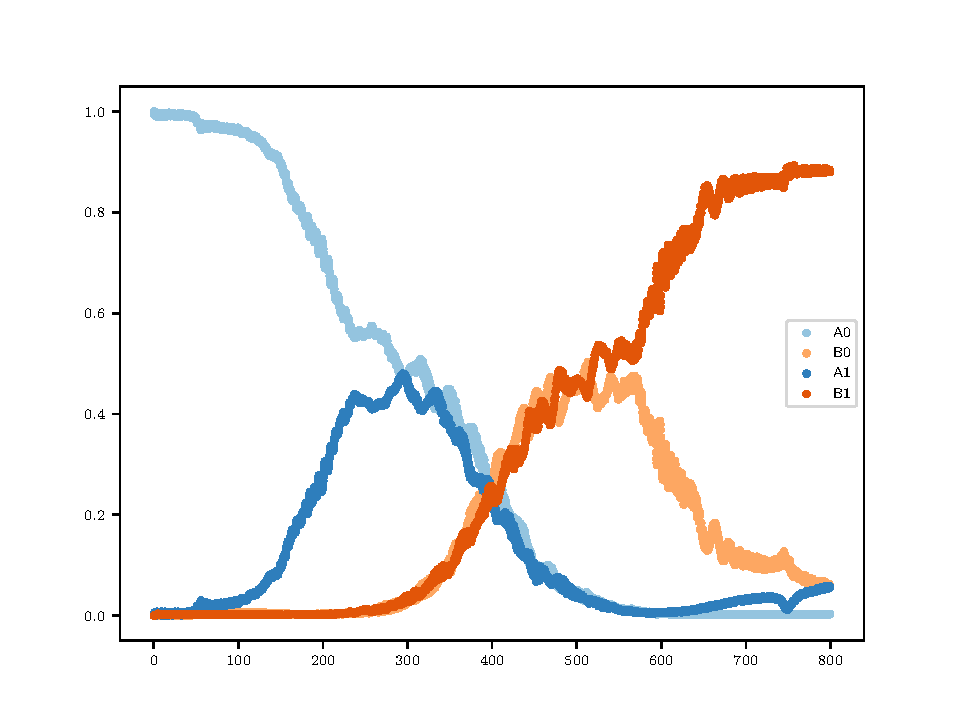
\includegraphics[width=\textwidth]{pictures/chain4_ricemele_1spto10oupling_doubletime_10phonons_Delta10.pdf}
        \caption{$\Delta=10$}
        \label{fig:image2}
    \end{subfigure}

    \caption{\textbf{longer time evolution for phonon number 10.}}
    \label{fig:both}
\end{figure}

% {	
% 	\thispagestyle{plain}

% 	\section*{Related publication}
% 	This thesis resulted from the research conducted in the master studies of the author. Parts of these results are already published in the following preprint:\\

% 	\begin{center}
% 		M. Cech, I. Lesanovsky, and F. Carollo, \\
% 		``Thermodynamics of quantum trajectories on a quantum computer'', \\
% 		\href{https://doi.org/10.48550/arXiv.2301.07124}{arXiv:2301.07124 (2023)},\\
% 		Submitted to \textit{Physical Review Letters} in January 2023.
% 	\end{center}
% 	\clearpage
% }
% \automark[section]{section}
% \lehead[\headmark]{\headmark}
% \rohead[\headmark]{\headmark}
% \printbibliography
% \input{chapters/appendices.tex}
% \cleardoublepage

% additional material  
%%%%%%%%%%%%%%%%%%%%%%%%%%%%%%%%%%%%%%%%%%%%%%%%%%%%%%%%%%%%%%%%%%%%%%%%%%%%%%%%%%%%%%%%%%%%%%%%%

{
	\thispagestyle{plain}
	\printbibliography
	\clearpage
}

% \input{chapters/appendices.tex}
% % \clearpage

% {
% 	\thispagestyle{plain}
% 	\chapter*{}
% 	\section*{Acknowledgements}
% 	First and foremost, I thank my two supervisors, Prof. Dr. Igor Lesanovsky and Dr. Federico Carollo. Your guidance, support, and mentorship have been invaluable throughout my master thesis and the related publication. After each of our discussions, I felt old questions answered and new ones raised.

% 	Of course, my gratitude also belongs to Prof. Dr. Daniel Braun, who appraised this thesis despite his current research semester.

% 	Also, I wish to extend my thanks to Priv.-Doz. Dr. Beatriz Olmos Sanchez, Chris Nill and Tom von Scheven. Your advices, encouragement and the professional exchange in each and every project during the last year provided me with a new perspective and have helped me approach problems from different angles. 

% 	Finally, I want to thank Moritz Eissler for proofreading this thesis and contributing valuable suggestions for its presentation. 
	
% 	\clearpage
	
% 	\thispagestyle{plain}
% 	\section*{Contact Information}
% 	Marcel Cech\\
% 	Institut für Theoretische Physik\\
% 	Auf der Morgenstelle 14\\
% 	Universität Tübingen\\
% 	72076 Tübingen\\
% 	Marcel.Cech@student.uni-tuebingen.de


% }

\end{document}